% Author :  Lionel du Peloux
% Contact : lionel.dupeloux@gmail
% Year : 2017

\chapter{Elastic gridshells}


\section{Building free-forms}
\subsection{Non-standard forms}
\subsection{Importance of free-forms in modern architecture}
\subsection{Canonical approaches to build free-forms}
\subsection{Main challenges}

\subsection{Elastic gridshell : a definition}

The invention of the gridshell concept is commonly attributed to Frei Otto, a German architect who devoted several years to gridshells. In 1975 he achieved the famous \emph{Mannheim Multihalle} \cite{Happold1975}, a wooden shell of 7500~m\textsuperscript{2}, in collaboration with the engineer Edmund Happold (Arup).
Literally, the word \textquote{gridshell} refers to grids behaving like shells~: from a mechanical point of view that means stresses acting on the structure are mainly transmitted through compression and traction. These structures can cross large-span with very little material.

However, according to the historic evolution of the concept, characterizing a gridshell as the combination of a structural concept -- a grid behaving like a shell -- and a specific construction process -- using the bending flexibility of the material -- seems to be more accurate. The Mannheim project (in which a wooden regular and planar grid, lacking shear stiffness, is elastically deformed up to a targeted shape with the help of stays, and then braced and covered) is regarded as the starting point of this new concept.

The Mannheim project is regarded as the starting point of this new concept for which a wooden regular and planar grid, lacking shear stiffness, is elastically deformed up to a targeted shape with the help of stays, and then braced and covered.
This type of gridshell, known as elastic gridshell, offers a very elegant manner to materialize freeform shapes from an initially flat and regular grid, which obviously has many practical benefits: planar geometry, standard connection nodes, standard profiles and so on.


\blockcquote[][p.~250]{IL10}{At present, the architectural significance of grid shells can hardly be fully envisioned. Too little experience has been gained as yet. However, the first signs of a grid shell architecture are already apparent. The projects planned and executed to date and the results of this research work indicate possibilities that open up a wide field of applications for grid shells. Two things stand out above all. The first is the nearly unlimited variety of forms that can be realized with grid shells, the second is the fact that there is no closed shell surface, but rather a simple, spatially curved grid composed of rods. Both features are of fundamental significance. They fully characterize the architectural essence of the grid shell support structure.}

\blockcquote[][p.~179]{IL10}{From the inverted form to the gridshell}


\clearpage

\clearpage


\section{Elastic gridshells : a thorough project review}

The \emph{IL10 Grid Shell} is a great source of information as it lists the early gridshell projects and give some valuable informations. Partial reviews can be found 

existing reviews : \citet{Quinn2014, Collins2016, Chilton2017, Adriaenssens2014}

\subsection{The beginnings : from the first prototype to the German Pavilion}
Frei Otto started his studies in architecture in 1947 in Berlin, Germany, and completed his doctorate on tensile structures in 1953. This first work was published and translated later in the 60's. He then began to work in the field of lightweight structures using physical models such as soap films or hanging nets, and photographic measurements.\footnote{In the 19\textsuperscript{th} and 20\textsuperscript{th} centuries model testing was at the heart of structural innovation \cite{Addis2013}. Analog models were employed successfully by well-known architects and engineers to go beyond the limits of existing knowledge (A. Gaudi, H. Isler, F. Candela, F. Otto, \telp{}) and are still employed today where numeric models failed to represent accurately some physical phenomenons (for instance in wind analysis for high rise towers and bridges).}\textsuperscript{,}\footnote{\blockcquote[p.~56]{IL10}{Photography is the medium through which the form and content of a model are communicated. It is one of our most important tools in that it provides the basis for documentation and information, supplements our creative potential \belp{} }} These tools were essentials for his exploration of forms and structures as there were no computers at that time.
\begin{figure}[h]
		\subfloat[][Knot detail]{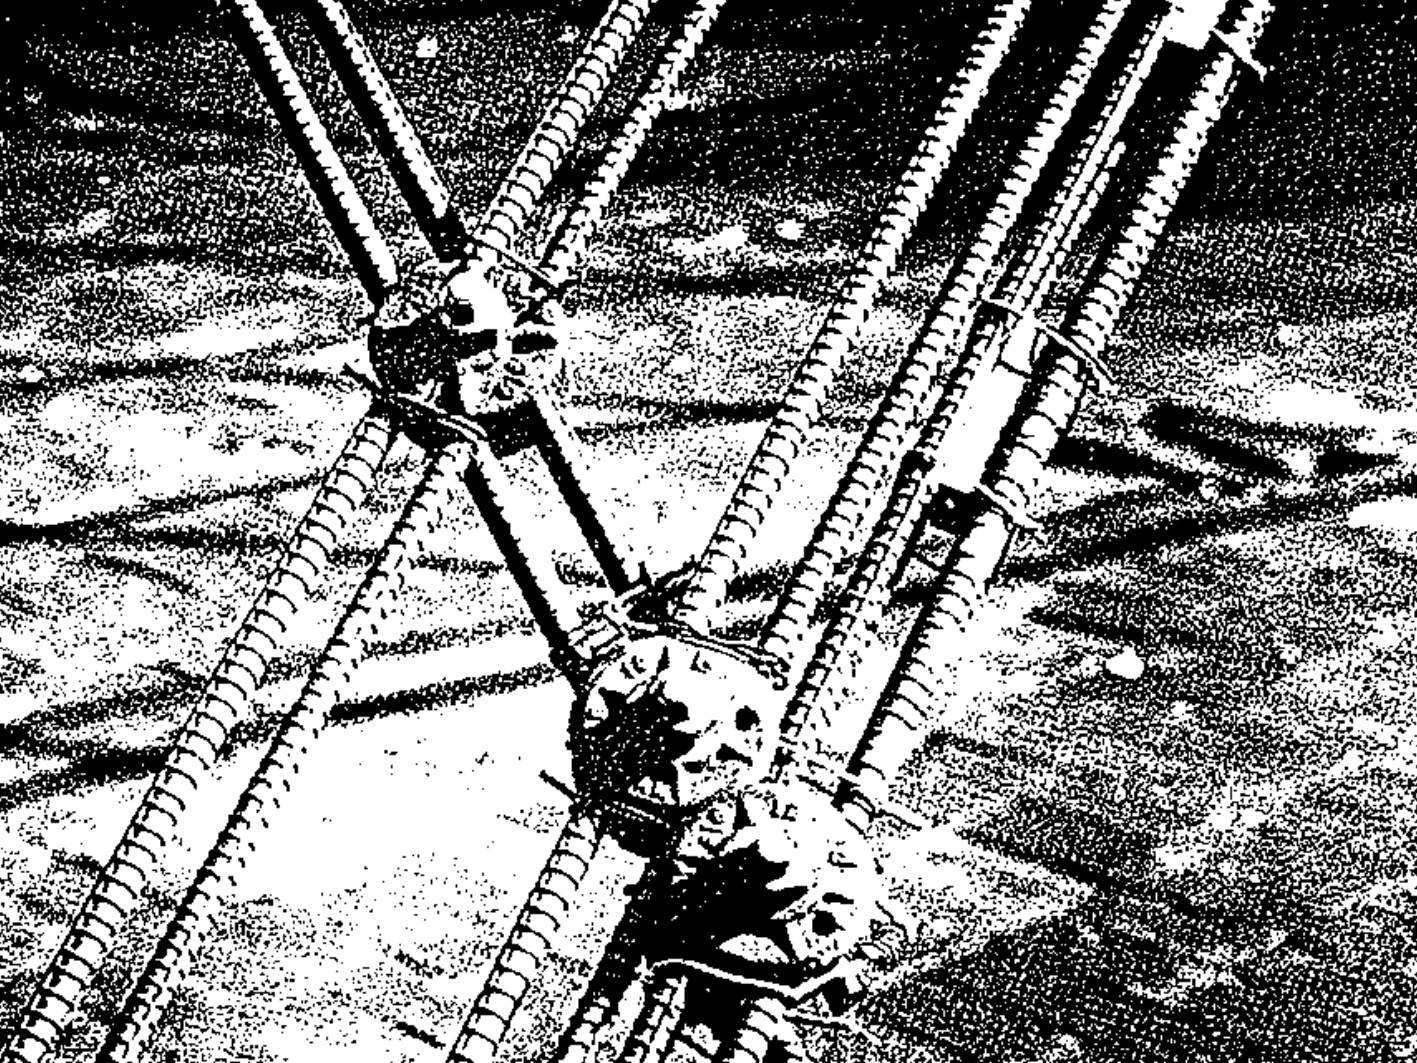
\includegraphics[width=0.48\textwidth]{berkeley_detail.jpg}\label{fig:berkeley_a}}
		\hspace*{\fill}
		\subfloat[][Steel lattice]{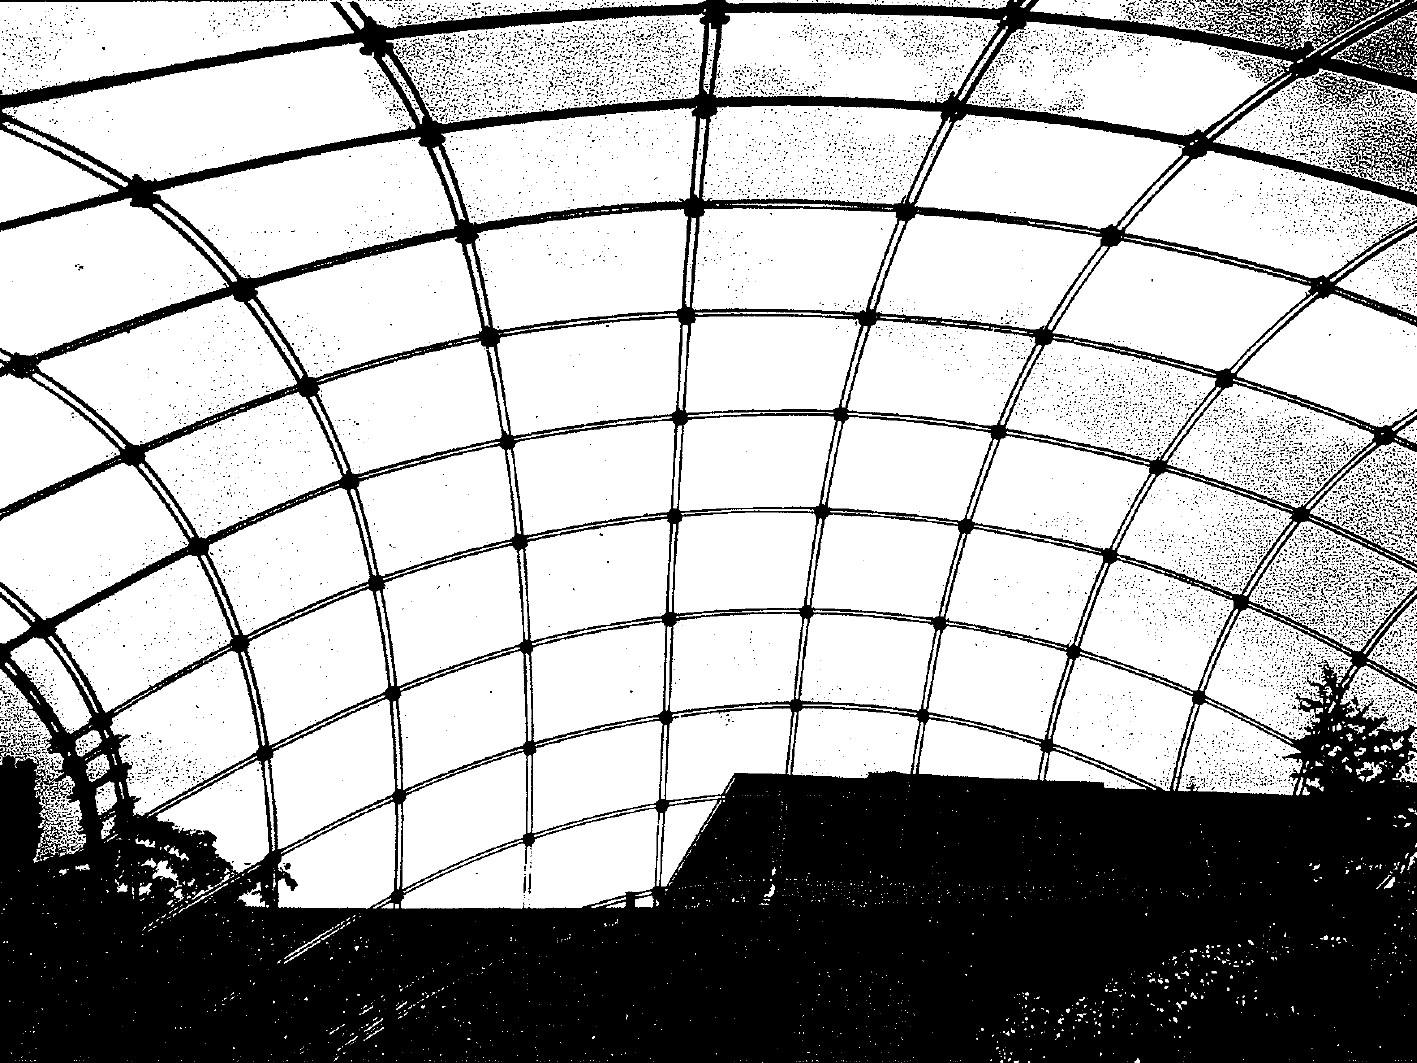
\includegraphics[width=0.48\textwidth]{berkeley_gs.jpg}\label{fig:berkeley_b}}
		%
		\vspace{10pt}
		\captionof{figure}[Steel gridshell built in 1962 in Berkeley, USA]{Steel gridshell built in 1962 in Berkeley, USA.}
		\label{fig:berkeley}    
\end{figure}

Simultaneously, he became interested by the study of lightweight shells and the way they were form-found. One of his very first elastic gridshell was built in 1962 with students at Berkeley, USA \cite[p.~270]{IL10}. It is funny to remark that this first gridshell was not a timber gridshell but a steel gridshell made out of twin steel rods linked in a grid fashion by bolts with clamping plates (see \cref{fig:berkeley_a}). This first experiment demonstrated at small scale the ability to bend a regular grid with no shear rigidity into a curved shape  (see \cref{fig:berkeley_b}). The grid was loosely braced and shell effects were not investigated.
\begin{figure}[p]
\begin{fullpage}
	\centering
	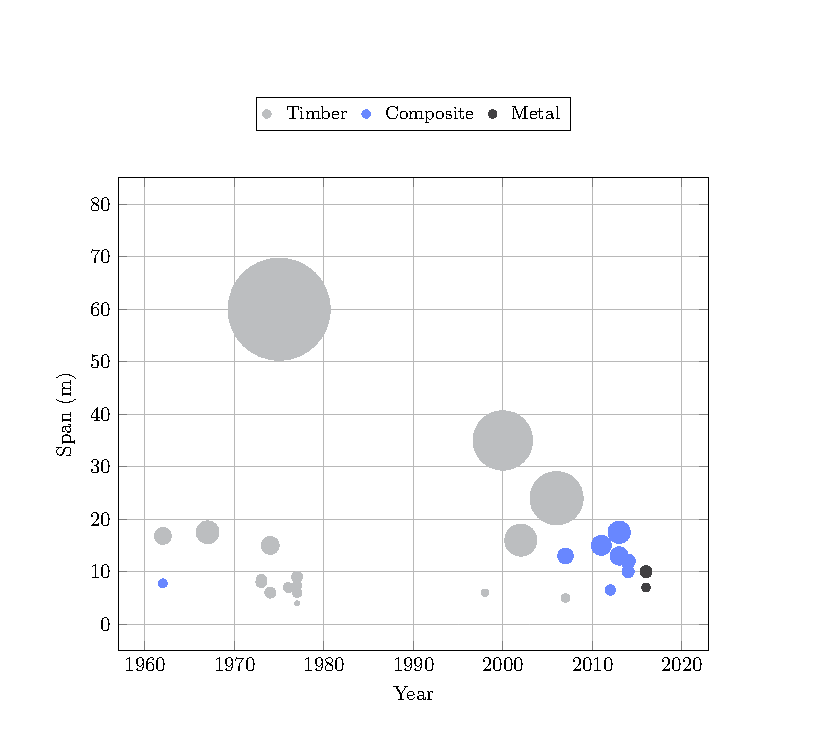
\includegraphics[]{ch1_gridshell/plot/1_projects/build.pdf}
	\caption[Known elastic gridshells built by the past.]{Known elastic gridshells built by the past. The surface of the bubbles is proportional to the covered area. Color indicates the material employed for the rods.}
	\label{fig:projectsbymaterial}
\end{fullpage}
\end{figure}

The same year he designed and built a first timber gridshell at Essen, Germany \cite[p.~272]{IL10}. The prototype~-- a single-layer gridshell spanning \SI{17}{m} and covering an area of \SI{198}{m^2} -- was made with 3-plies laminated timber profiles in hemlock pine (see \cref{fig:essen_a}). The cross-section of the profiles was rectangular (\SI{60}{mm} x \SI{40}{mm}) and the elements were assembled in a grid fashion with simple steel bolts. Once erected, nothing was specifically done to improve the in-plane shear stiffness of the grid and activate a shell behavior. Finally, the structure was covered with a transparent plastic foil nailed directly on the grid's profiles (see \cref{fig:essen_b}).
\begin{figure}[h]
		\subfloat[][Timber lattice]{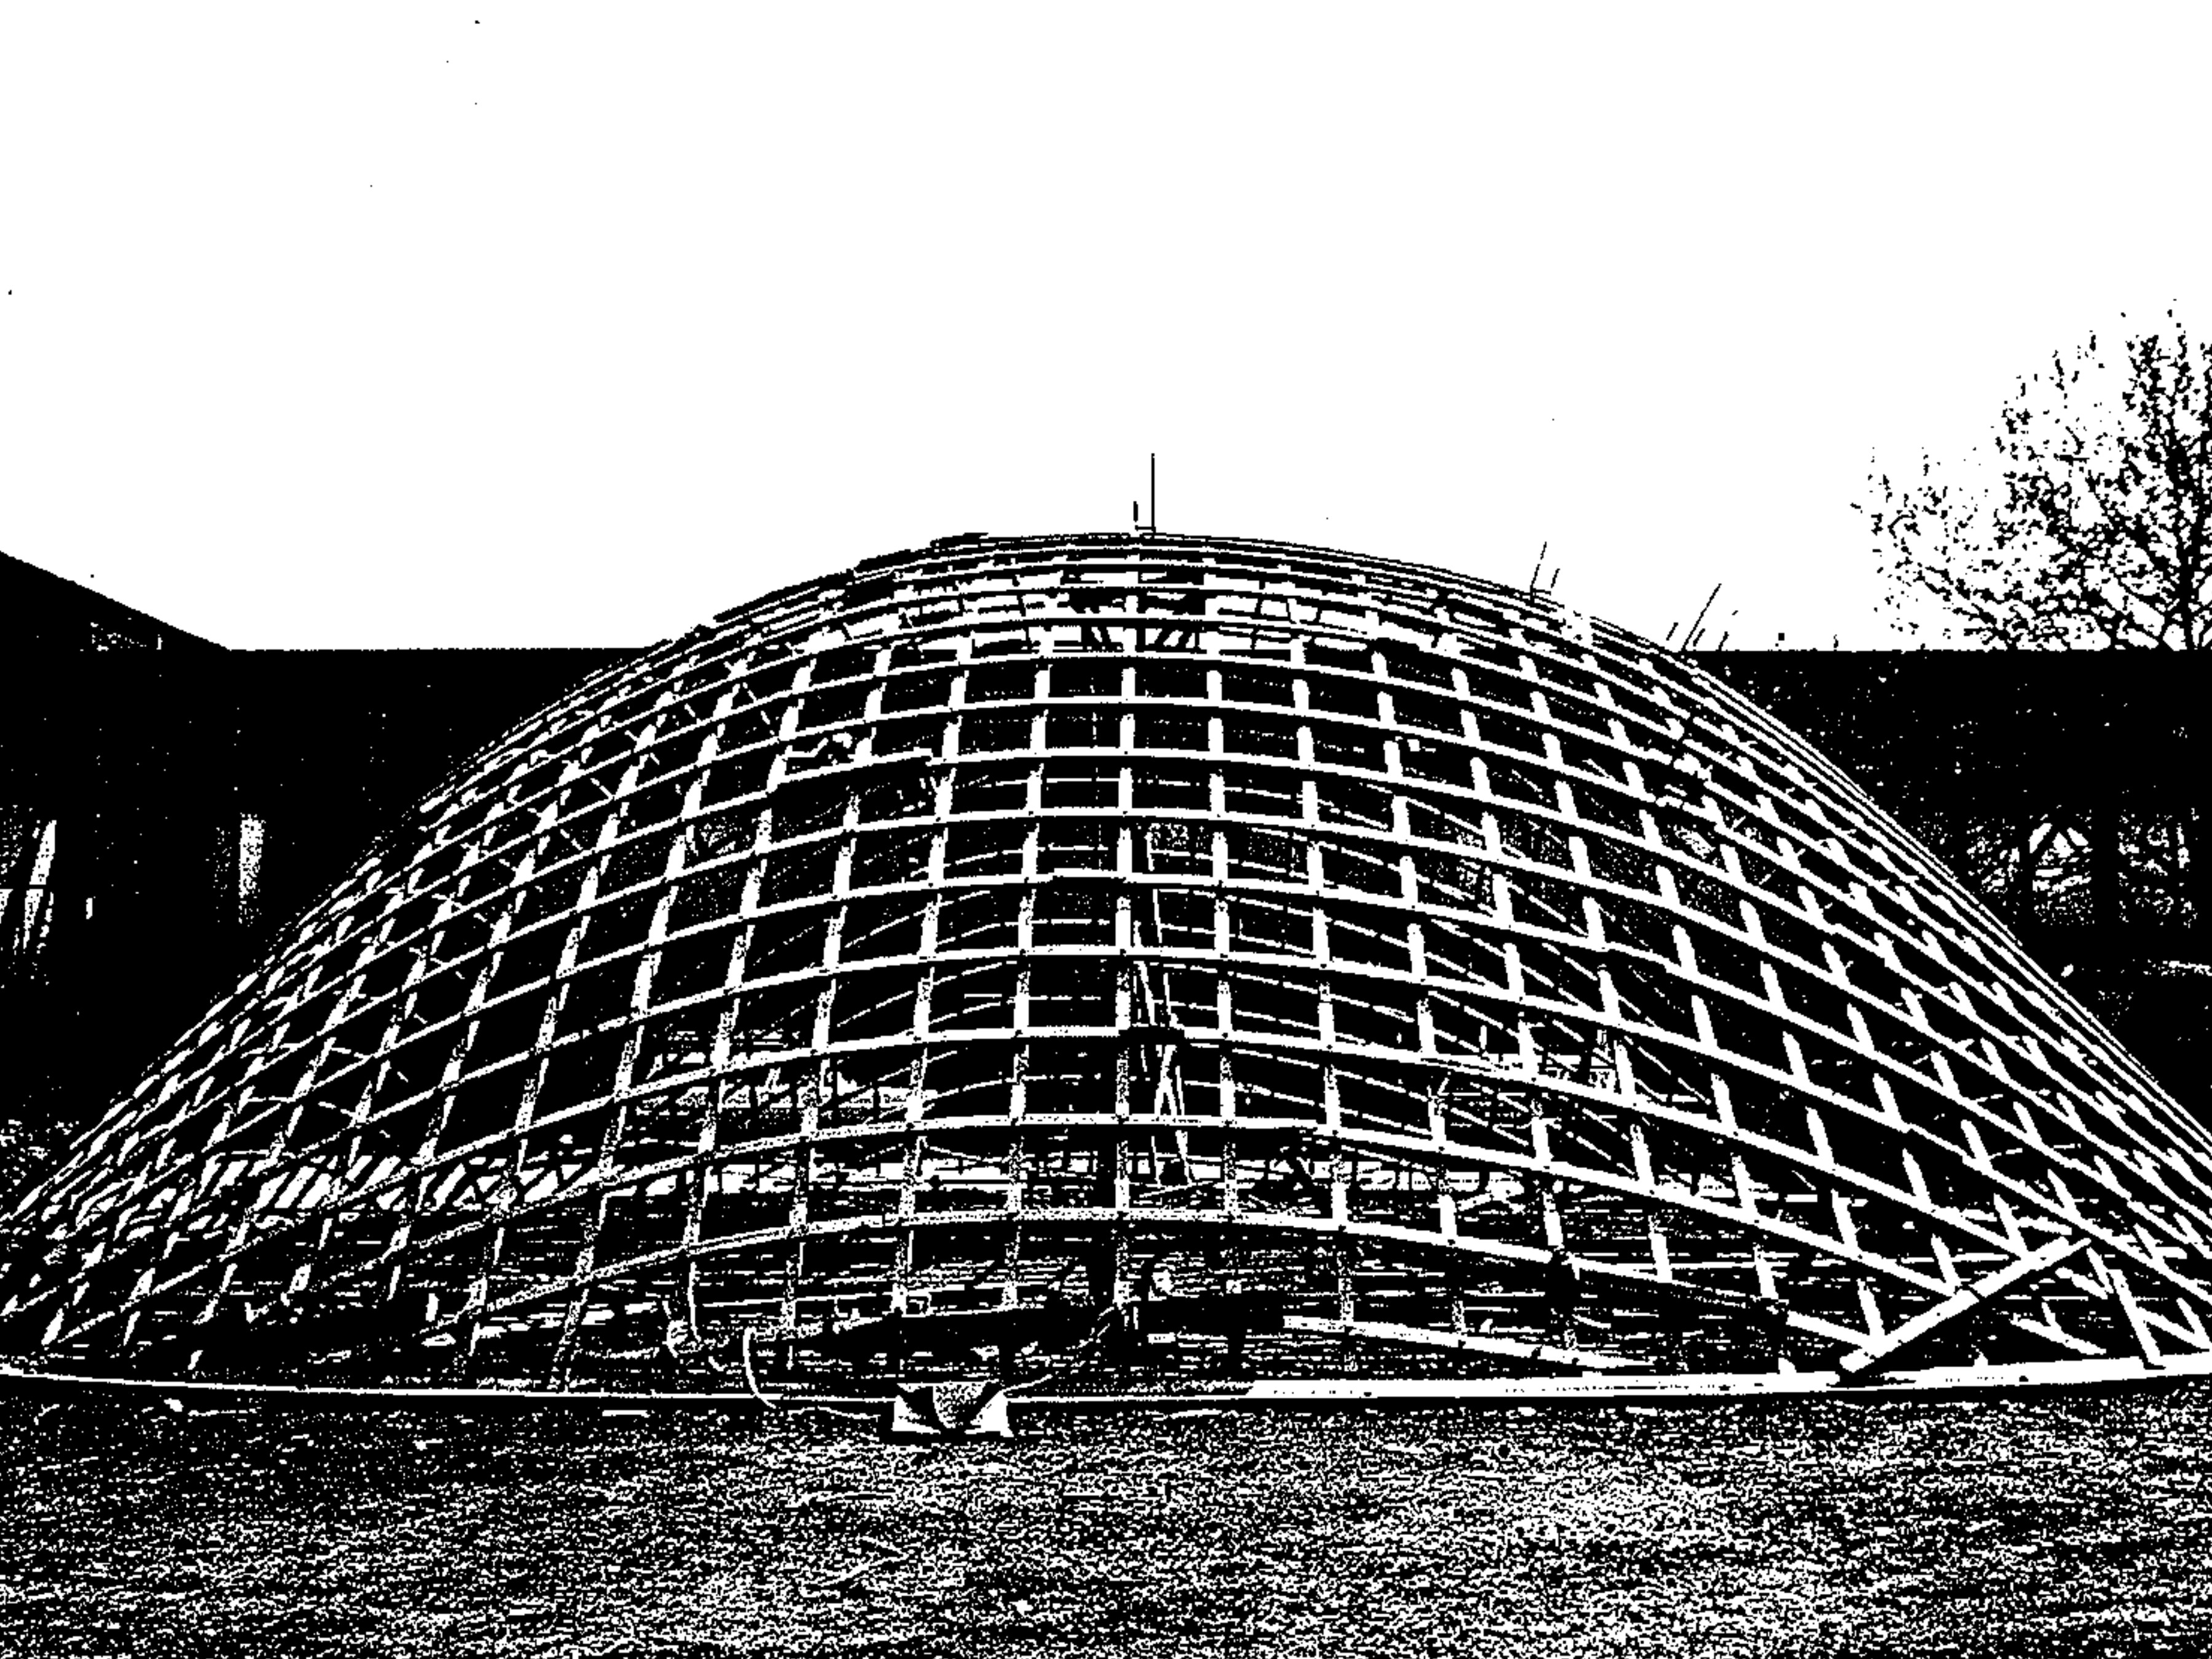
\includegraphics[width=0.48\textwidth]{essen_gs.jpg}\label{fig:essen_a}}
		\hspace*{\fill}
		\subfloat[][Plastic foil]{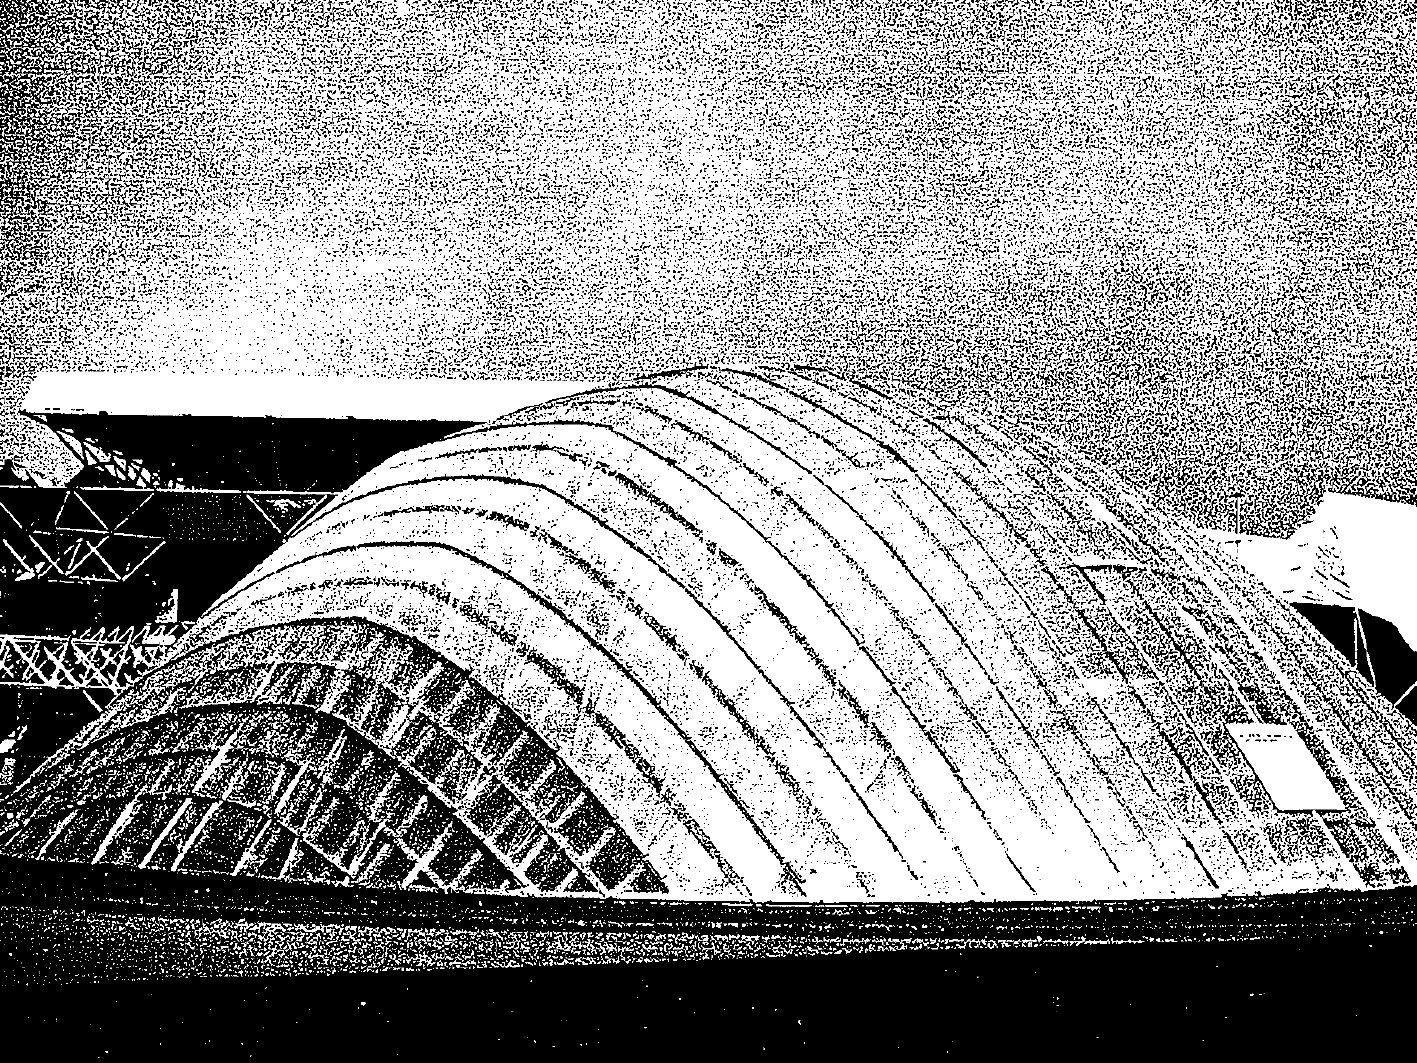
\includegraphics[width=0.48\textwidth]{essen_foil.jpg}\label{fig:essen_b}}
		%
		\vspace{10pt}
		\captionof{figure}[Timber gridshell built in 1962 in Essen, Germany]{Timber gridshell built in 1962 in Essen, Germany.}
		\label{fig:essen}    
\end{figure}
Fiver years later, on the occasion of the \emph{1967 International and Universal Exposition} in Montreal, Canada, Frei Otto was appointed to design the German Pavilion~: a large cable net tent prefiguring the realization of the olympic stadium of Munich, Germany, in 1972.\footnote{Actually, Frei Otto became the director of the newly founded \emph{Institute for Lightweight Structures} (Institut für Leichte Flächentragwerke or IL) at the University of Stuttgart in 1964. It was the IL that was commissioned by the German government to conduct research in connection with the planning of the German pavilion for the exposition in Montreal.} The pavilion required two auditoria and these were designed using the principle of elastic gridshell \cite[p.~274]{IL10}. All together, the auditoria covered and area of \SI{365}{m^2} and spanned \SI{17.5}{m}. The construction technique employed in Montreal was quite similar to the one developed in Essen, but this time the grid was fully braced with a layer of nailed plywood boards and offered a proper roofing made out of insulation panels covered with a PVC coated fabric (see \cref{fig:montreal_a,fig:montreal_b}).

The two gridshells built in Montreal mark a significant step in the maturation process of the technique leading to the major realization of Mannheim in 1976~: a methodology has emerged to progress \blockcquote[p.~179]{IL10}{from the inverted form to the gridshell} ; main construction details have been validated ; various erection methods have been tested ; mid-scale buildings have been built to host public. However, due to the over complexity of these structures, lots of unknowns remained unsolved at this stage and the behavior of the structures could not be fully predicted.\footnote{\blockcquote[p.~219]{IL10}{Snow accumulations in the throat of the common edge beam probably caused one of the two grid shells of project Montreal to buckle in a relatively flat region. The diameter of the buckled area was about 3 meters. Neither grid rod was broken, i.e. the buckling progressed elastically. It might have been possible to press the buckled area back into shape.}}
\begin{figure}[h]
		\subfloat[][Grid erection]{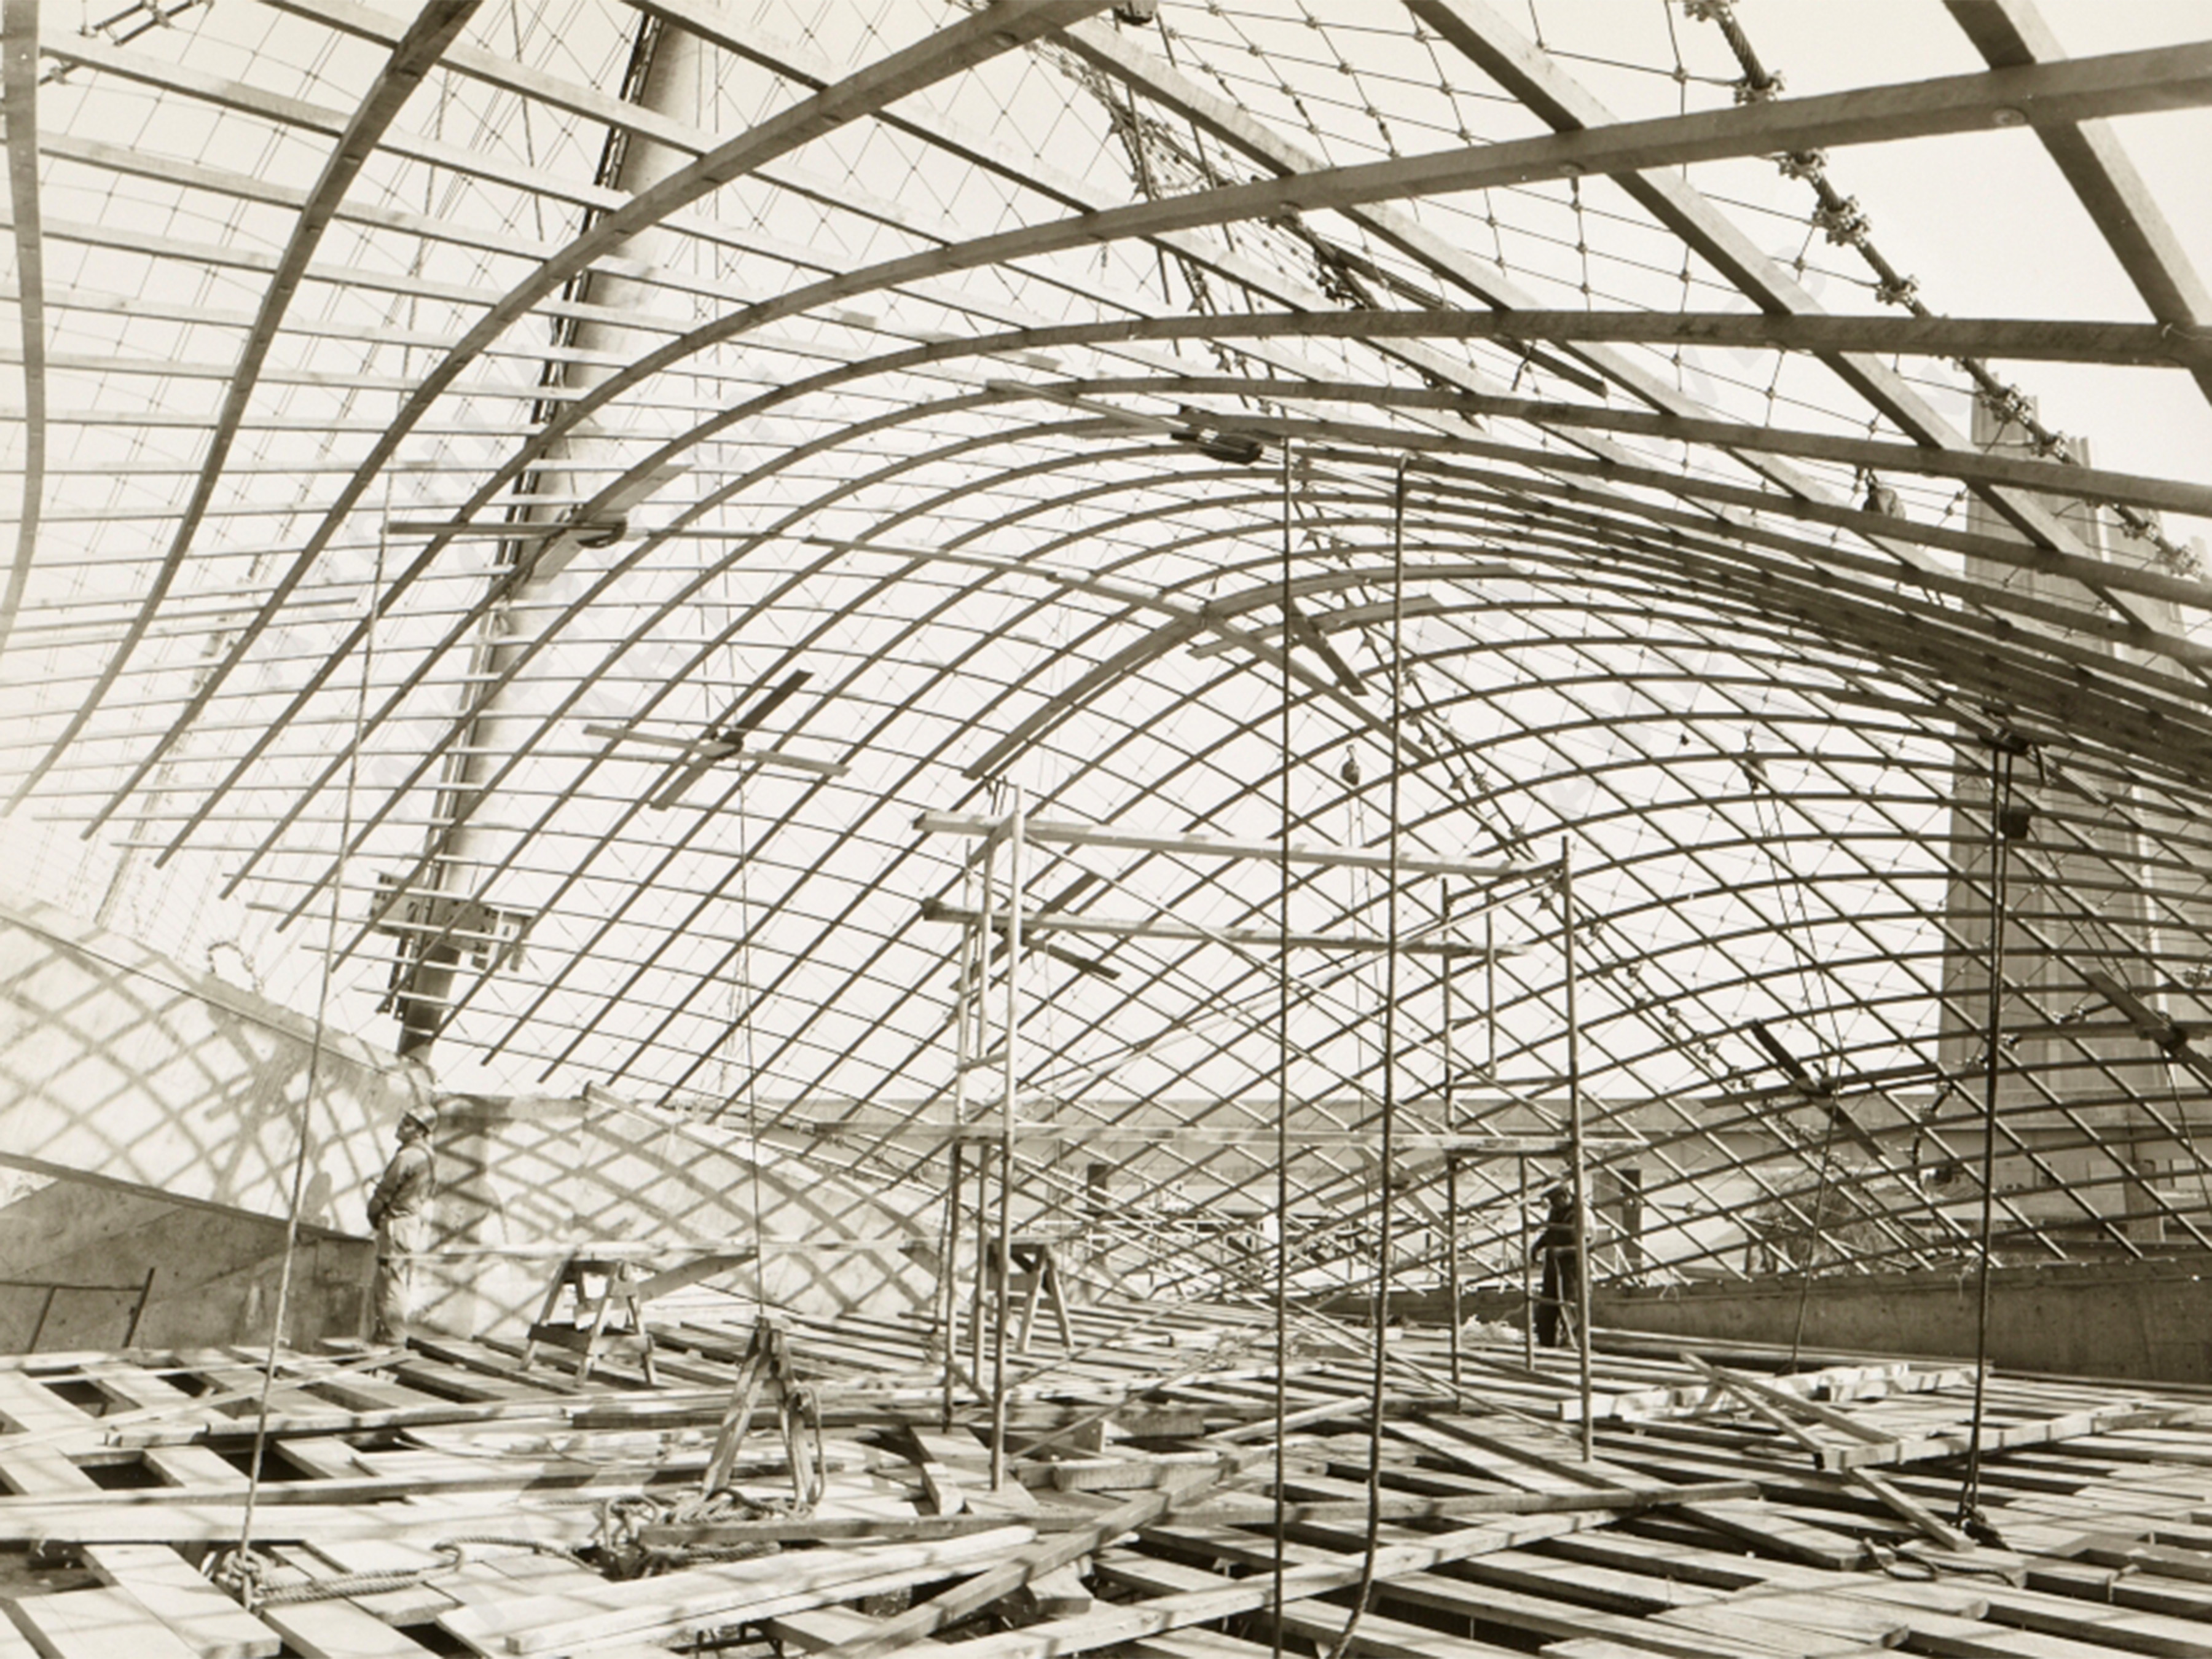
\includegraphics[width=0.48\textwidth]{montreal_lift.jpg}\label{fig:montreal_a}}
		\hspace*{\fill}
		\subfloat[][Interior view]{\includegraphics[width=0.48\textwidth]{montreal_int.jpg}\label{fig:montreal_b}}
		%
		\vspace{10pt}
		\captionof{figure}[Timber gridshell built in 1967 in Montreal, Canada]{Timber gridshell built in 1967 in Montreal, Canada.}
		\label{fig:montreal}    
\end{figure}

It is worth to mention that several unexecuted large-scale projects were studied by Frei Otto between 1967 and 1973 at the \emph{IL} or at the \emph{Atelier Warmbronn}.\footnote{Atelier Warmbronn is the architectural studio founded by Frei Otto in 1969.} These projects are basically documented in \cite[pp.~278 - 288]{IL10} and reveal that he was training his capacity to master large-scale projects with the technique of elastic gridshells for more conventional building projects (wave pool, swimming hall, multi-purpose hall, auditorium, \telp{}).

\subsection{Mannheim Multihalle : the completion of a decade of research}
The project of the Multihalle started in 1970, when the decision was made that Mannheim, Germany, would hold the Bundesgartenschau in 1975.\footnote{The Bundesgartenschau is a national horticultural exibithion that takes place every two years in Germany.} The architects of the project, \emph{Carl Mutschler \& Partners}, consulted Frei Otto at \emph{Atelier Warmbronn} as he was starting to get known in the filed of innovative lightweight structures. This is how the idea of the gridshell was introduced in the project \cite{Liddell2015}. 

A thorough report on the project is available in \cite{IL13}.  A more condensed but still precise description of the engineering problematics related to this projects are availlables in the excellent papers from \citet{Happold1975, Liddell2015}.
\begin{figure}[h]
		\subfloat[][Interior view]{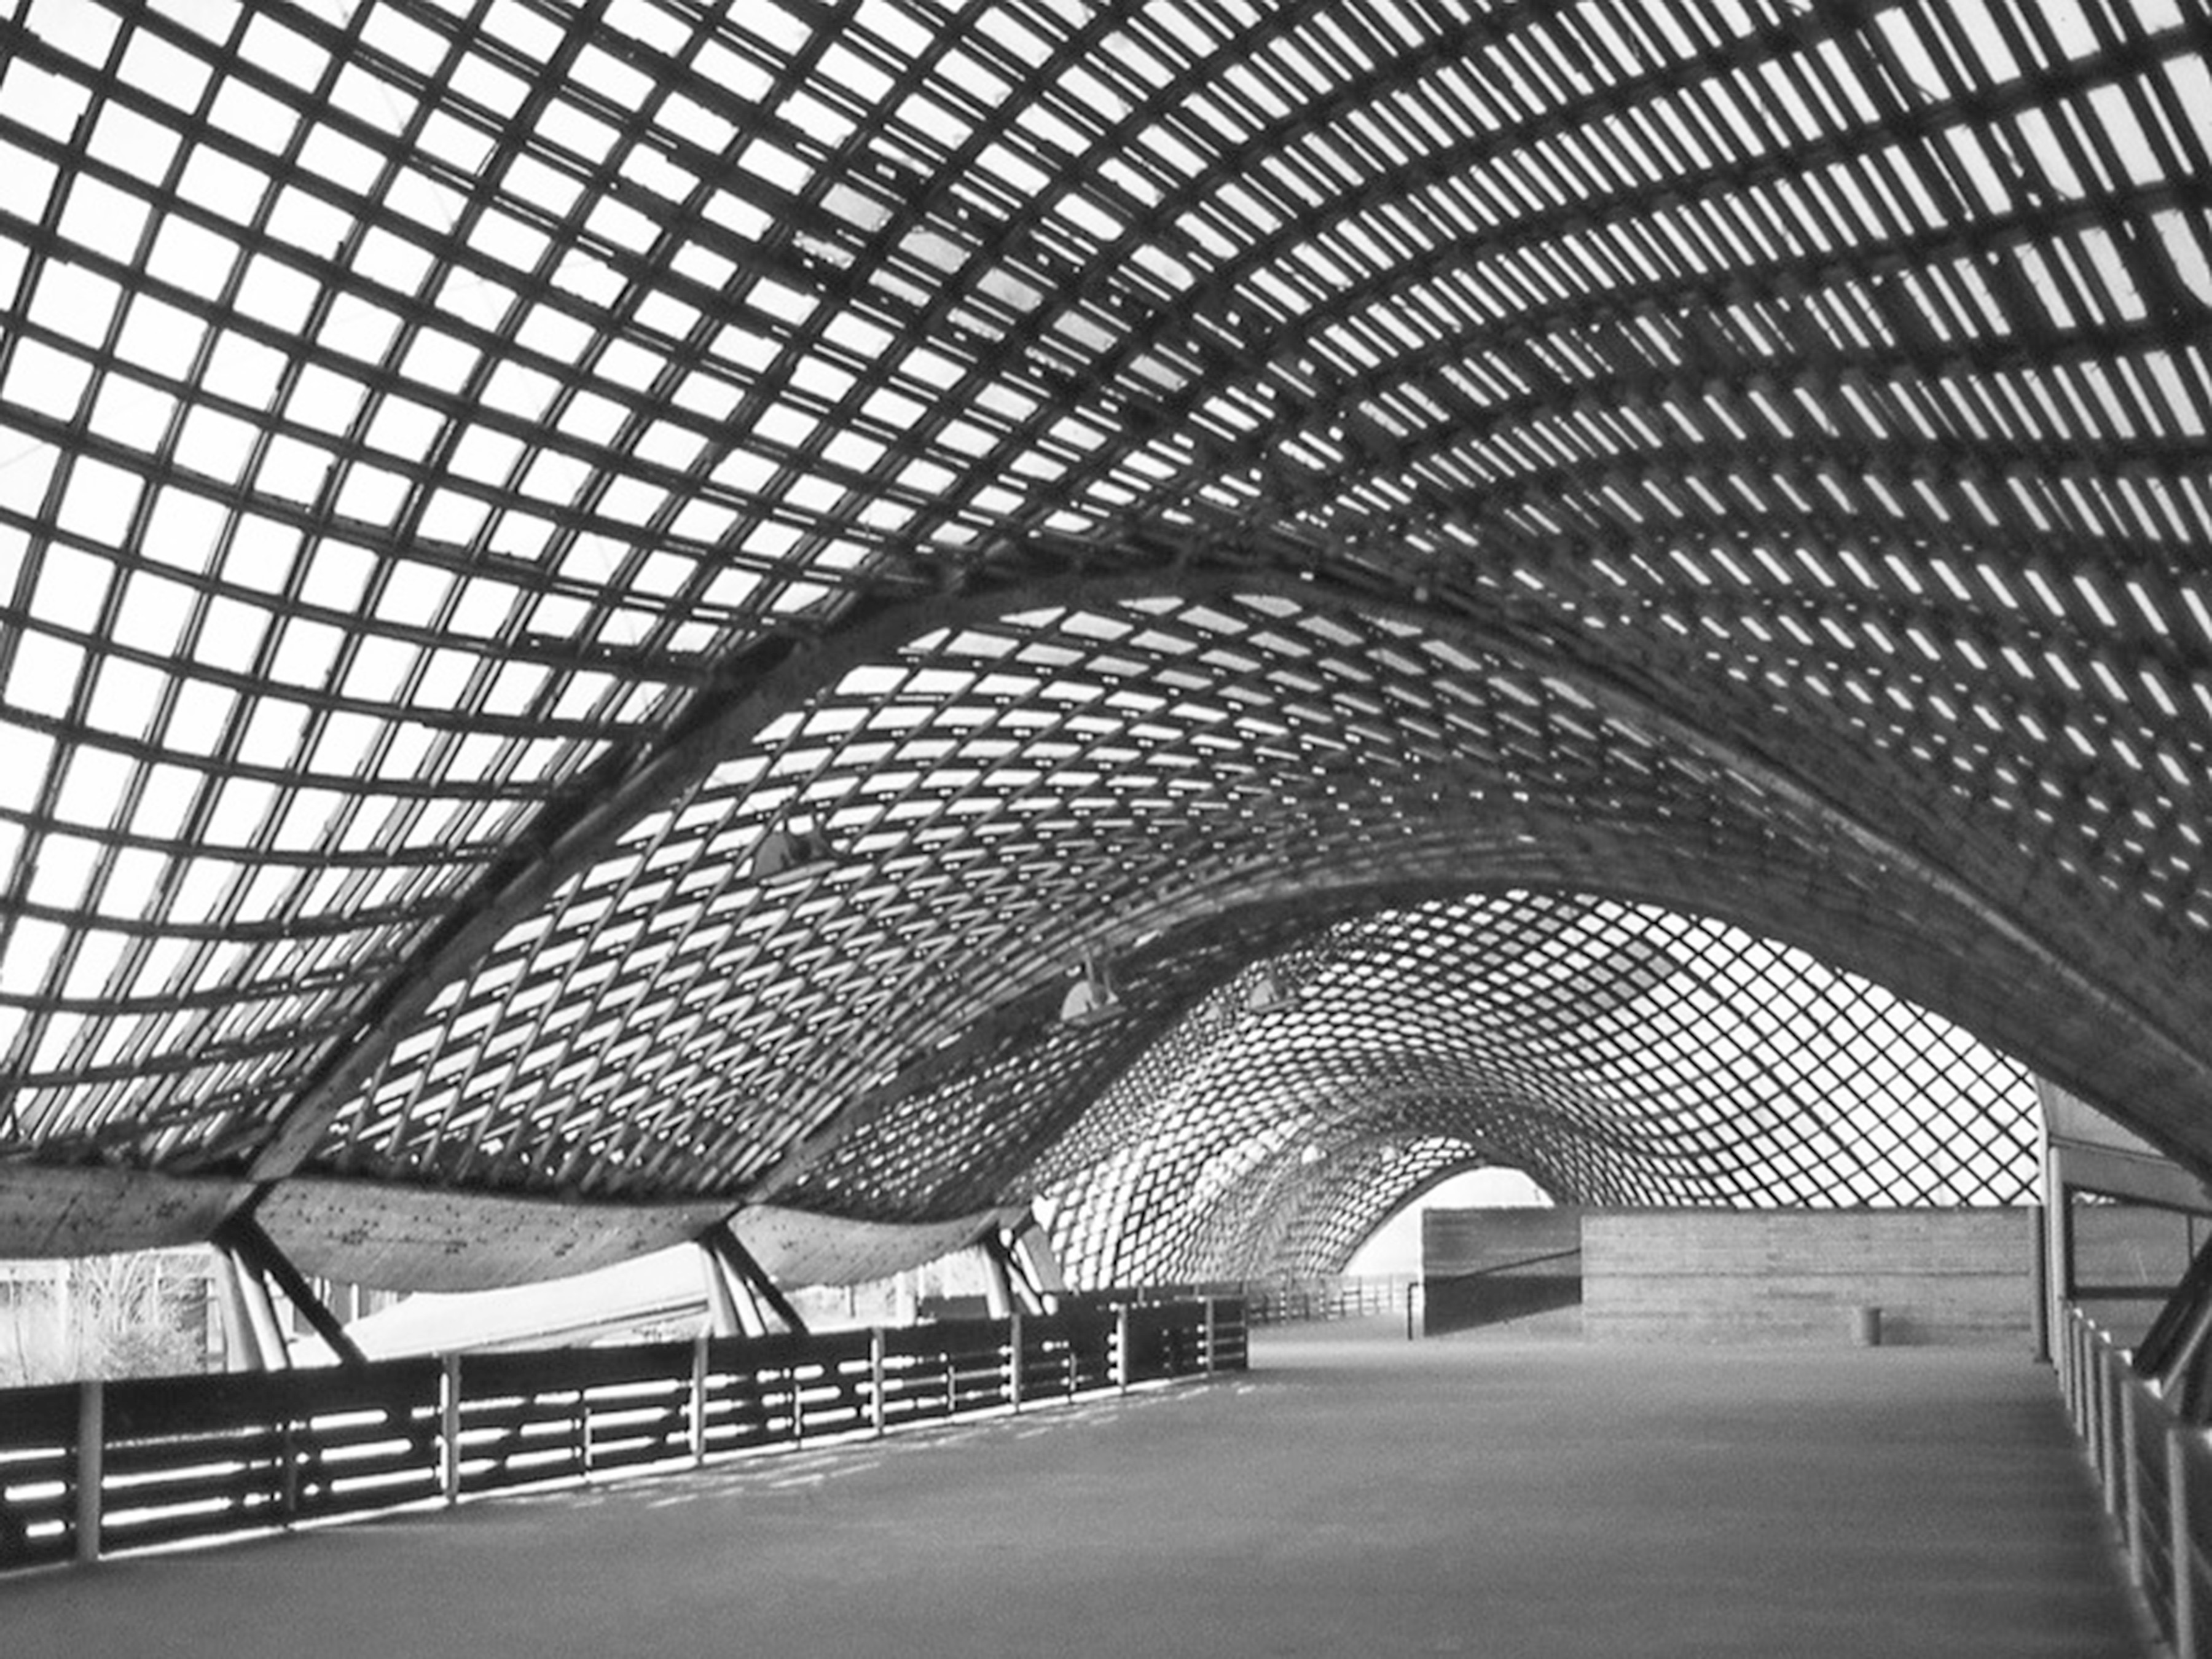
\includegraphics[width=0.48\textwidth]{mannheim_int.jpg}\label{fig:mannheim_a}}
		\hspace*{\fill}
		\subfloat[][Sky view]{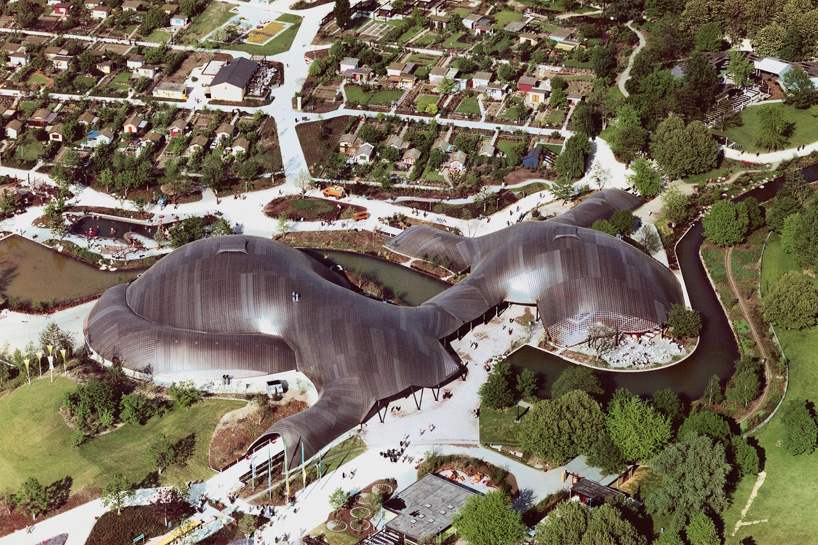
\includegraphics[width=0.48\textwidth]{mannheim_sky.jpg}\label{fig:mannheim_b}}
		%
		\vspace{10pt}
		\captionof{figure}[Timber gridshell built in 1962 in Essen, Germany]{Timber gridshell built in 1975 in Mannheim, Germany.}
		\label{fig:mannheim}    
\end{figure}

Mannheim is an unprecedented realization because it is more than twenty times larger than the previously built gridshells in Montreal and is meant to last many years and not only for the duration of a short-term exhibition. The timber lattice, still existing in 2017,  covers an area of \SI{7400}{m^2} (see \cref{fig:mannheim_b}). It is composed of two interconnected domes, one for the multi-purpose hall (span : \SI{60}{m} | height : \SI{20}{m}) and one for the restaurant (span : \SI{50}{m} | height : \SI{18}{m}).

Although the constructif system deployed at Mannheim clearly inherited from the previous developments, the challenge was such that it had to be revisited. In particular the main additions were the introduction of the double-layer system and the proper bracing of the grid. A major advance was also the use of the very first numeric models to study the structure. 

The double-layer system was introduced to tackle a two issues~: the grid needed some flexibility to be bent into the desired shape, but once erected it should provide sufficient bending stiffness to resist disturbing loads and avoid a buckling collapse.\footnote{Theoretically, self-weight loads would produce only compression in the members because the (funicular) form of the grid resulted from the inversion of a hanging chain model in pure tension.} One erected, the two grids, one sliding on top of the other one, were connected together to form a single grid with much higher ladder profiles (from \SI{50}{mm} to \SI{150}{mm}), increasing their bending stiffness by 26 (see \cref{fig:mannheim_a}).

Because the in-plane stiffness of the grid also plays a major role in the resistance to buckling, this question was considered with care. The bracing of the grid was first achieved by preventing the nodes to turn once the grid was erected. This was done by creating some friction in the nodes when tightening the bolts linking the laths, after the grid was erected. Additional bracing cables were put in the grid.

Finally, the project of Mannheim was a key project in the development of modern lightweight structures. Great engineers were born in touch with Frei Otto, following its footsteps or collaborating with him. This heritage has irrigated for several decades the engineering of lightweight structures in Europe and gave birth, directly or indirectly, to several studios among which we can cite \emph{Buro Happold}, \emph{Schlaich Bergermann \& Partner} and \emph{RFR}.

\subsection{The dry period : 25 years from Mannheim to Hannover}

Although the experience of Mannheim proved the feasibility and the potential of gridshell structures for large-scale projects, it also revealed that these projects were subject to an incredible complexity in terms of structural design, geometry, modeling, testing, team work, construction methods, \telp{} At that time, very few people could pretend to master all the knowledge and techniques required to design and built timber gridshells and developed in the bosom of the \emph{Institute for Lightweight Structures} in Stuttgart. 

This project was obviously well ahead of its time and the engineering cost to design such structures was probably prohibitive considering the tools available at that time. This certainly explains why no elastic gridshells were built during the 25 following years, despite the optimism of the pioneers of the Multihalle.\footnote{\blockcquote[]{Harris2003}{For many years after its completion, Happold promoted the benefit of the timber gridshell as a construction technique and stated that he could not understand why it had not been adopted more widely. He perceived the benefits to be in the efficiency of the construction method to enable doubly curved (shell) structures to be constructed quickly and cost effectively.}.}

Note that around 1975 small workshop and experiments lead to the construction of several but small elastic gridshells, as reported in \cite{IL10}. A non-exhaustive but quite extensive list of known executed gridshell projects is presented in \cref{fig:projectsbymaterial}. The dry period is clearly visible.

\subsection{The signs of a renewal : Dorset and Doncaster}\label{sec:signs}

It is only 20 years later that gridshells started to reappear., in the late 90's.

\subsubsection{Westminster Lodge, Dorset, England, 1995}
\begin{figure}[t]
		\subfloat[][Interior view]{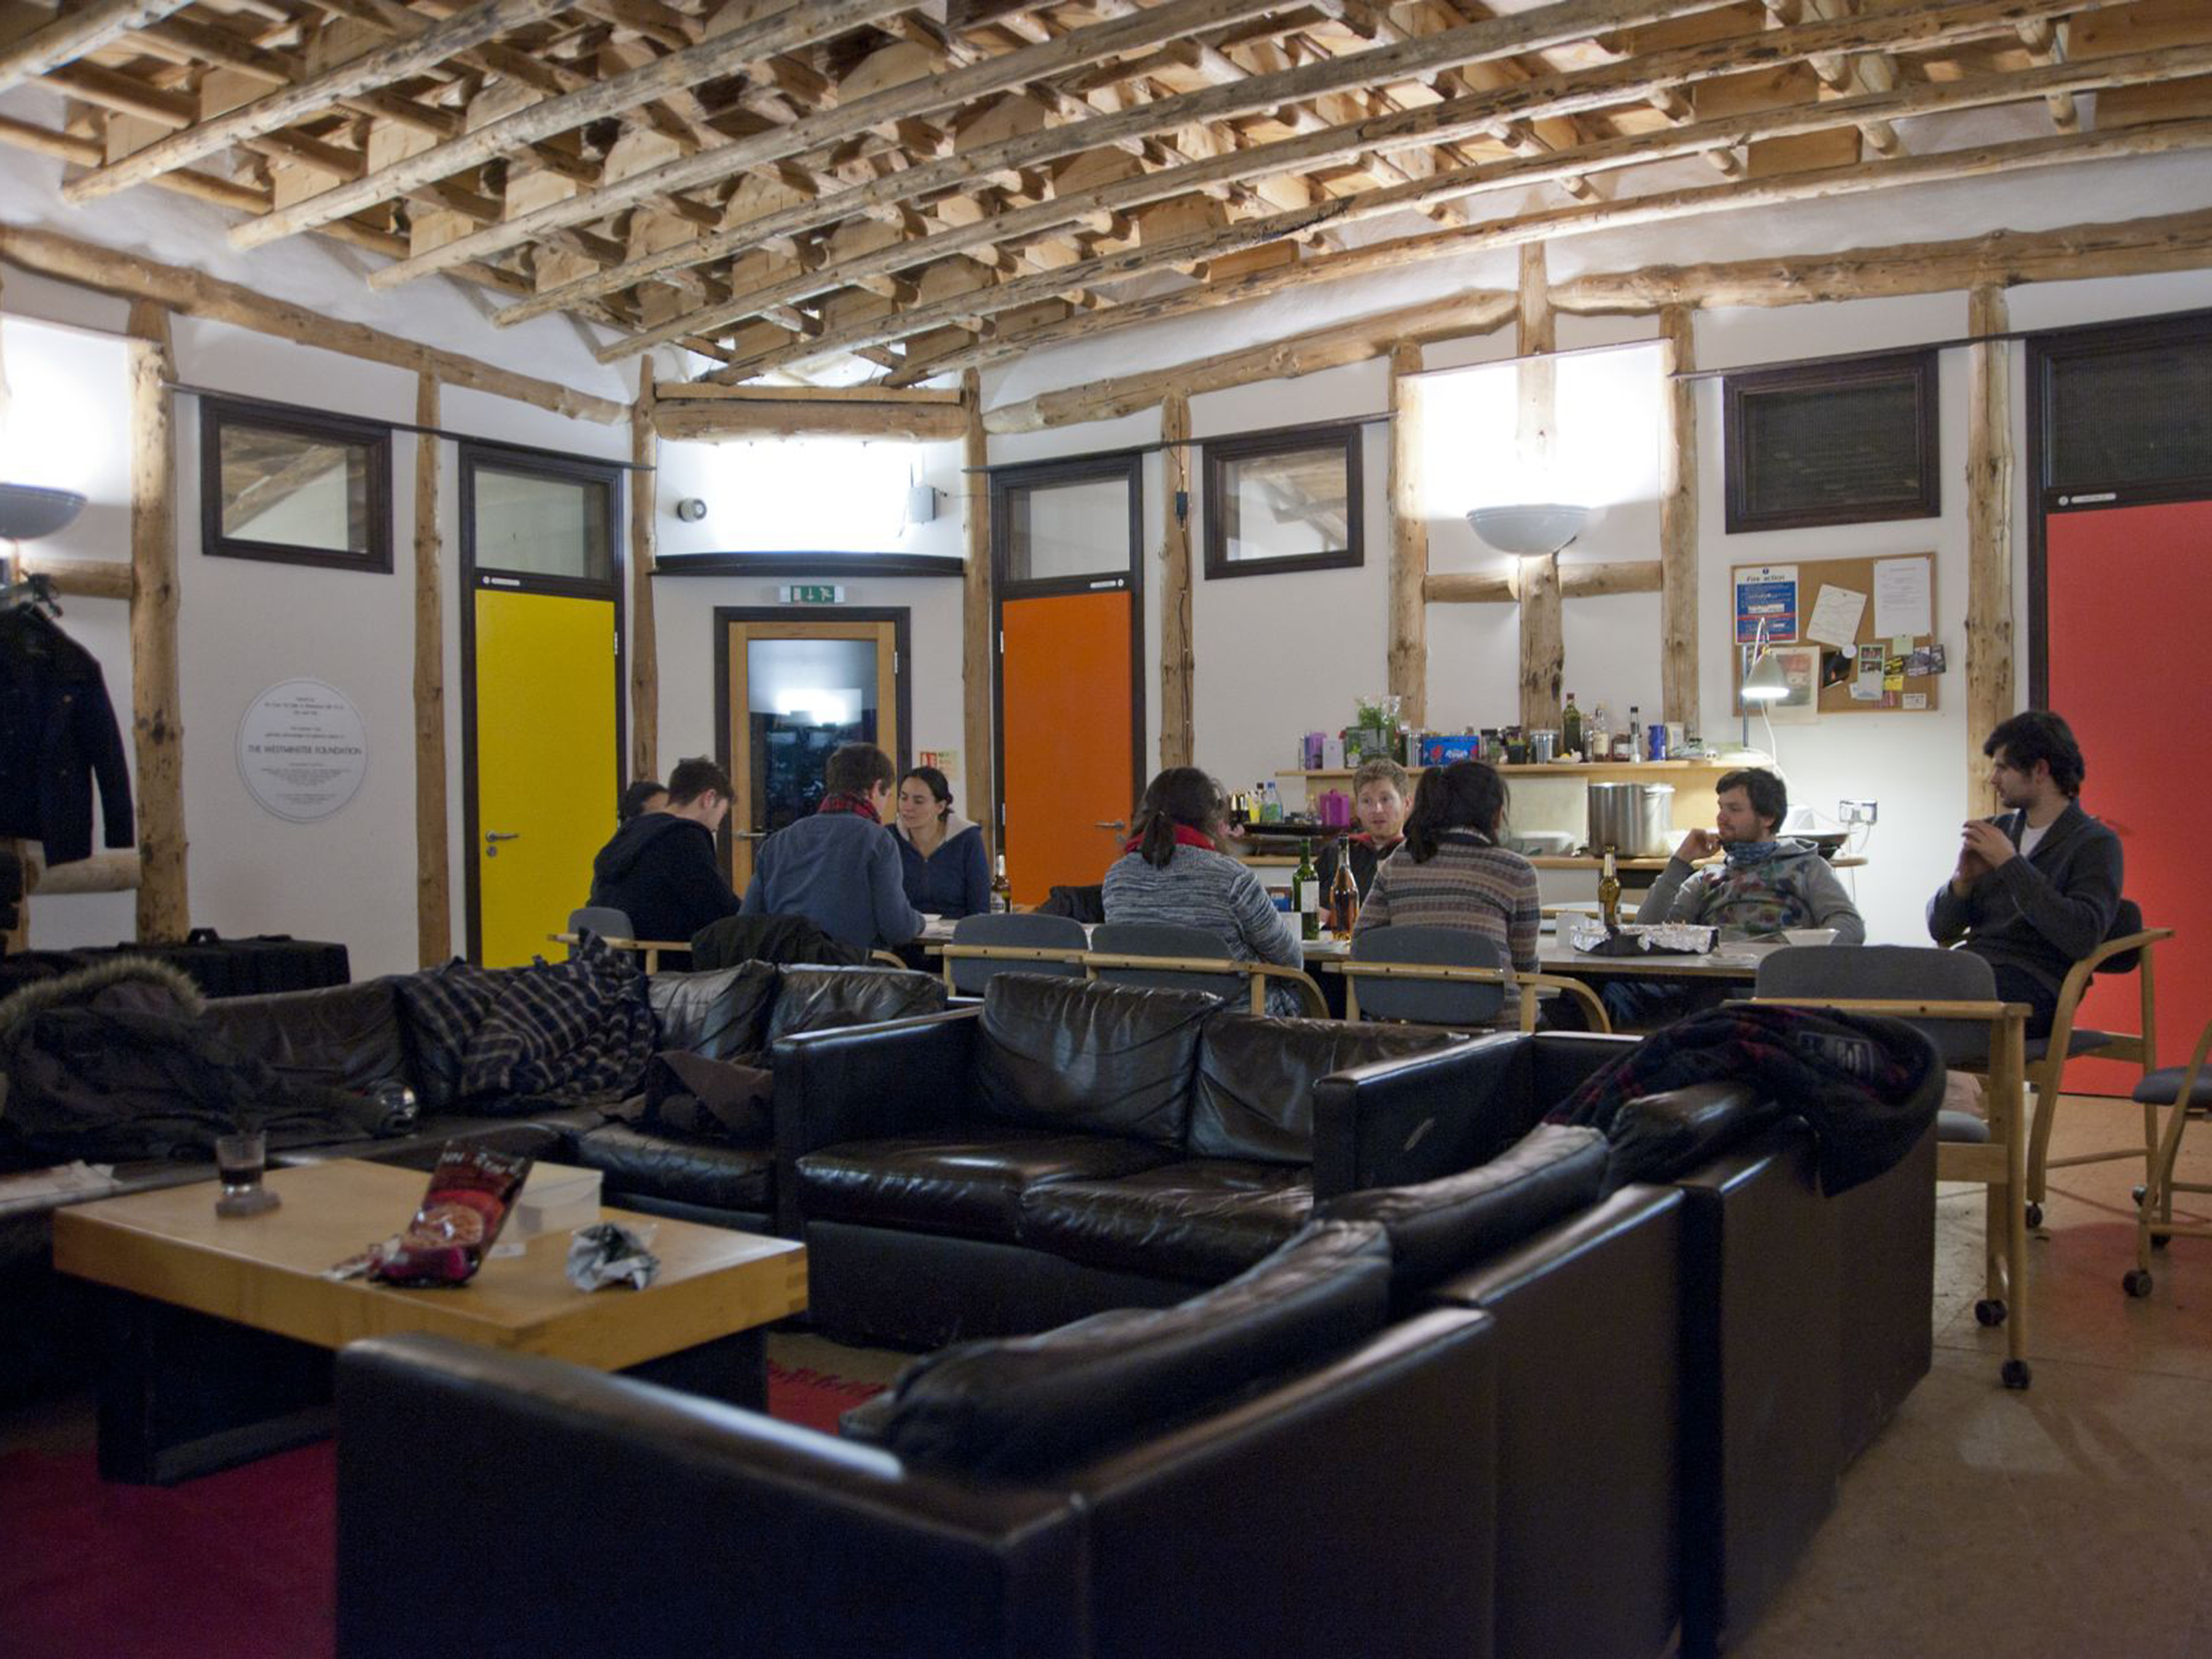
\includegraphics[width=0.48\textwidth]{dorset_int.jpg}\label{fig:dorset_a}}
		\hspace*{\fill}
		\subfloat[][Exterior view]{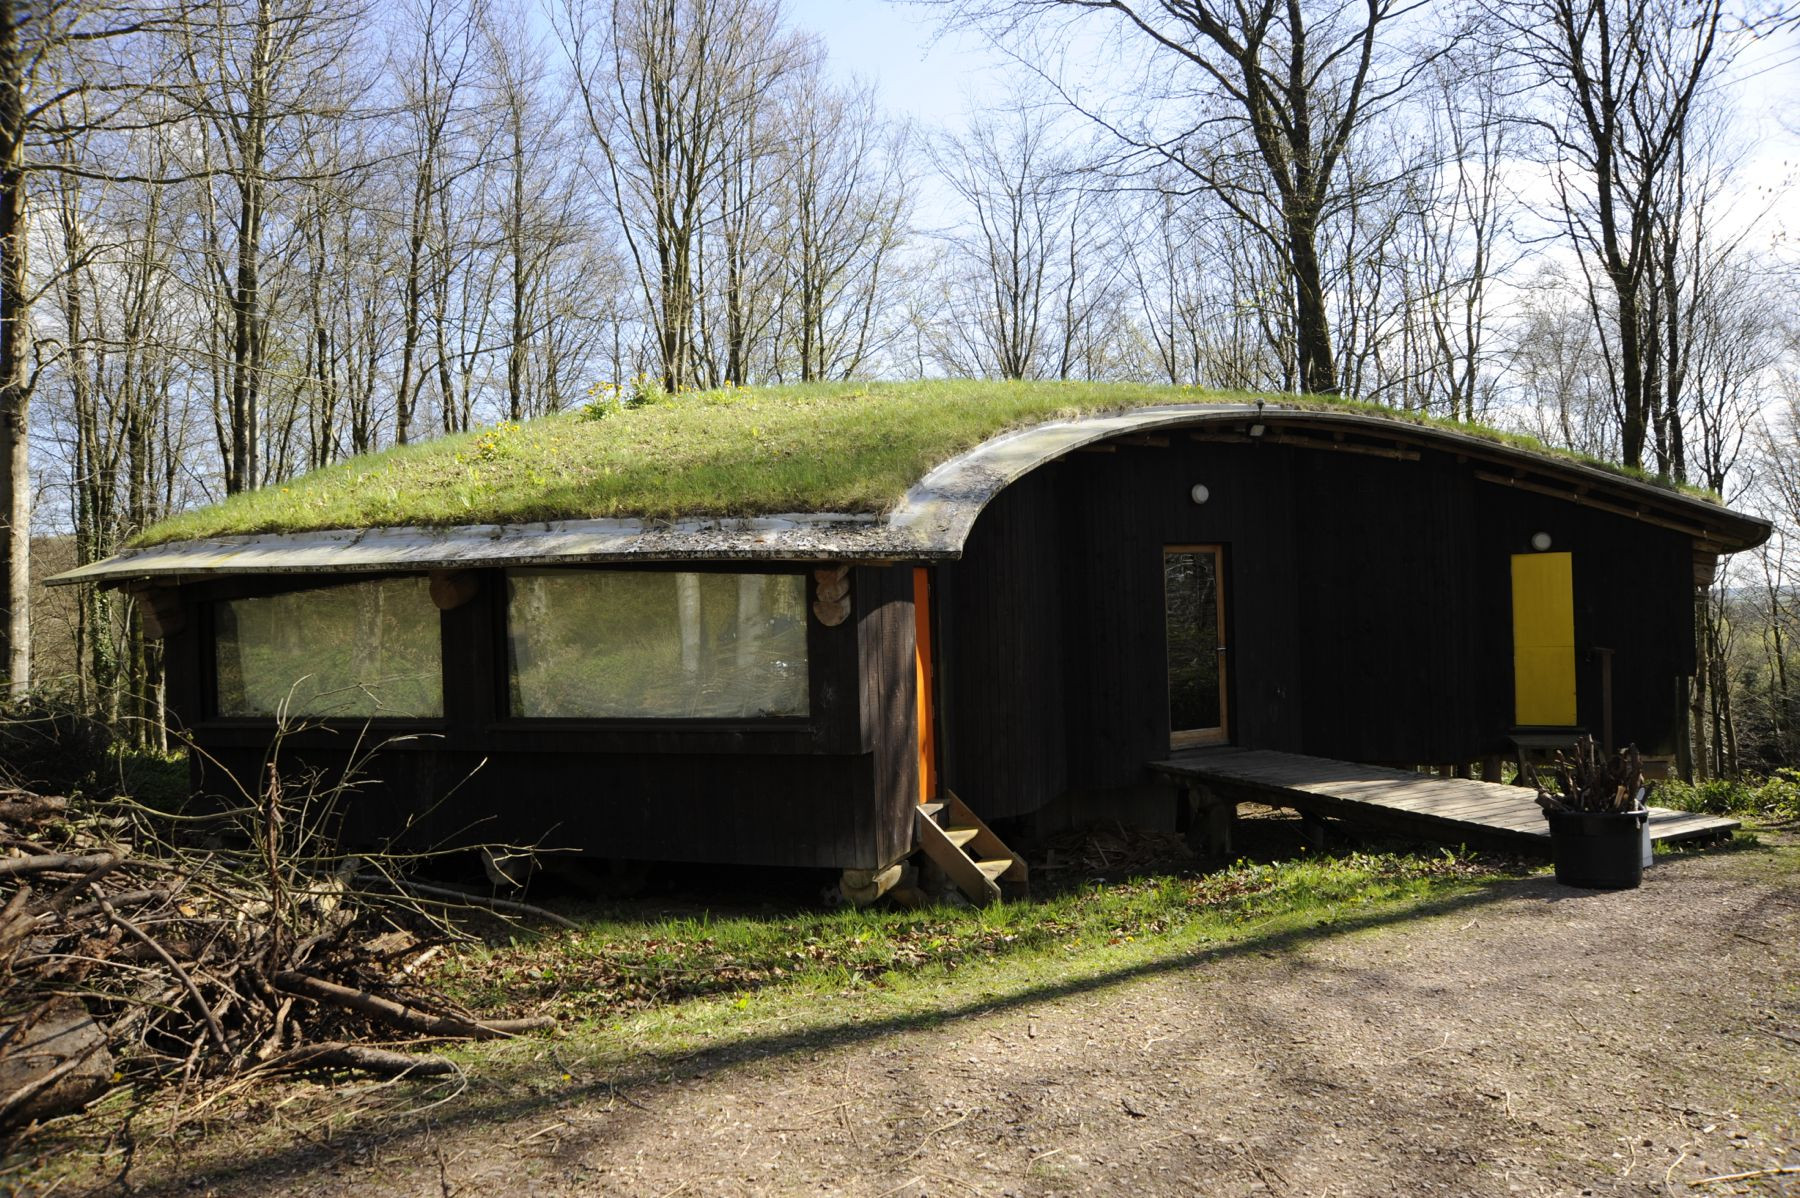
\includegraphics[width=0.48\textwidth]{dorset_ext.jpg}\label{fig:dorset_b}}
		%
		\vspace{10pt}
		\captionof{figure}[Roundwood gridshell built in 1995 in Dorset, England]{Roundwood gridshell built in 1995 in Dorset, England.}
		\label{fig:dorset}    
\end{figure}
In 1995, a small student residence named \emph{Westminster Lodge} was built in Dorset, England. This dwelling was part of a larger project -- Hooke Park -- aiming at investigating how the local forest resources, in particular immature roundwood  thinnings, could be better utilized. The project was lead by ABK, Frei Otto, Buro Happold and Cullinan Studio. Unlike Mannheim, the timber shell was bent and weaved rod by rod on a scaffold platform. But the structural system exhibited a double-layer gridshell pattern very similar to the one employed for the Multihalle (see \cref{fig:dorset_a}). The rods were made out of splice-jointed roundwood to form long-length poles of diameter \SI{200}{mm}. The development of this jointing technique, which could be produced directly in the forest, was part of the project's investigations \cite{Burton1998}. The grid was braced by a layer of diagonal boards nailed to the roundwoods. The structure was finally cladded with a planted turf roof (see \cref{fig:dorset_b}).


\subsubsection{Earth Center, Doncaster, England, 1998}
At the same time, a project of a similar spirit arose for the \emph{Earth Center} in Doncaster, England.\footnote{\textquote{\href{http://grant-associates.uk.com/approach/earth-centre-forest-garden-grid-shells/}{The Earth Centre Forest Garden} was intended to demonstrate how managed woodland could supply the vast majority of all natural resources needed for human survival.}} The project planning started in 1994 and a series of small timber gridshells were designed by Buro Happold and then built in 1998. The landscape structures were single-layer timber gridshells made with oak laths. Once erected with a crane, the grids were braced with crossing diagonal stainless steel cables (see \cref{fig:doncaster_a}). Openings were possibly reinforced with curved timber frames (see \cref{fig:doncaster_b}).
\begin{figure}[h]
		\subfloat[][Interior view]{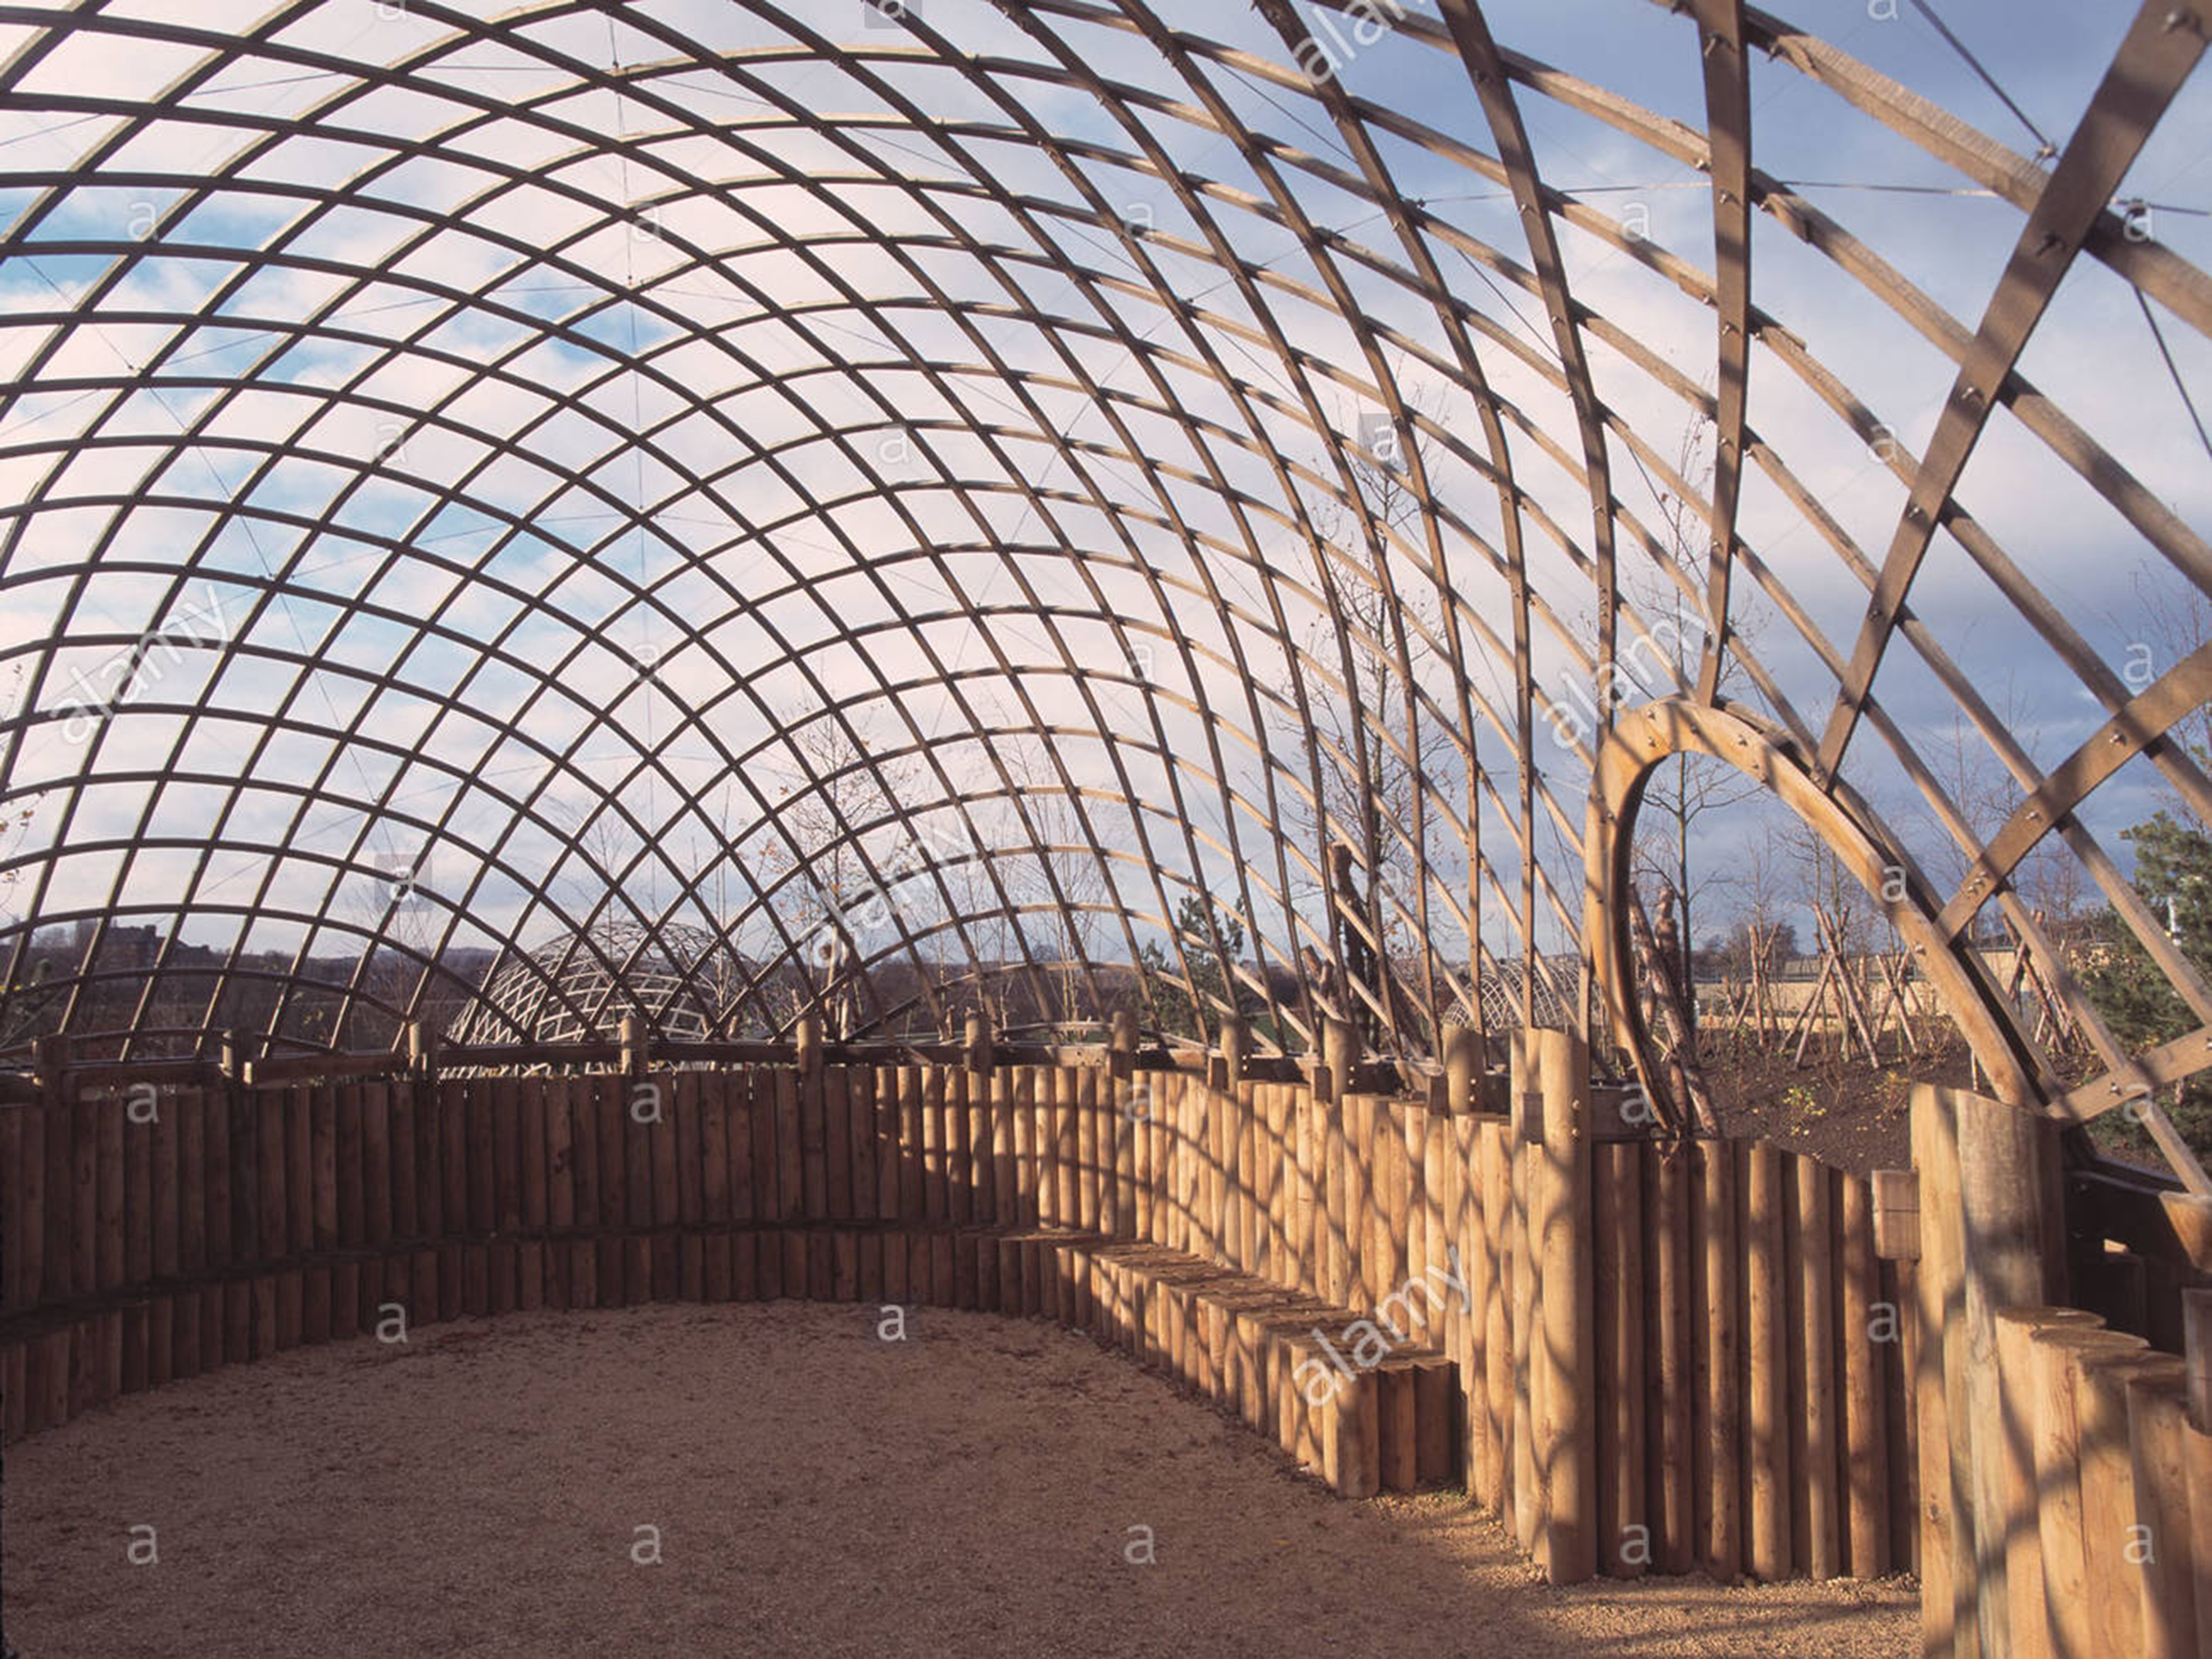
\includegraphics[width=0.48\textwidth]{doncaster_int.jpg}\label{fig:doncaster_a}}
		\hspace*{\fill}
		\subfloat[][Exterior view]{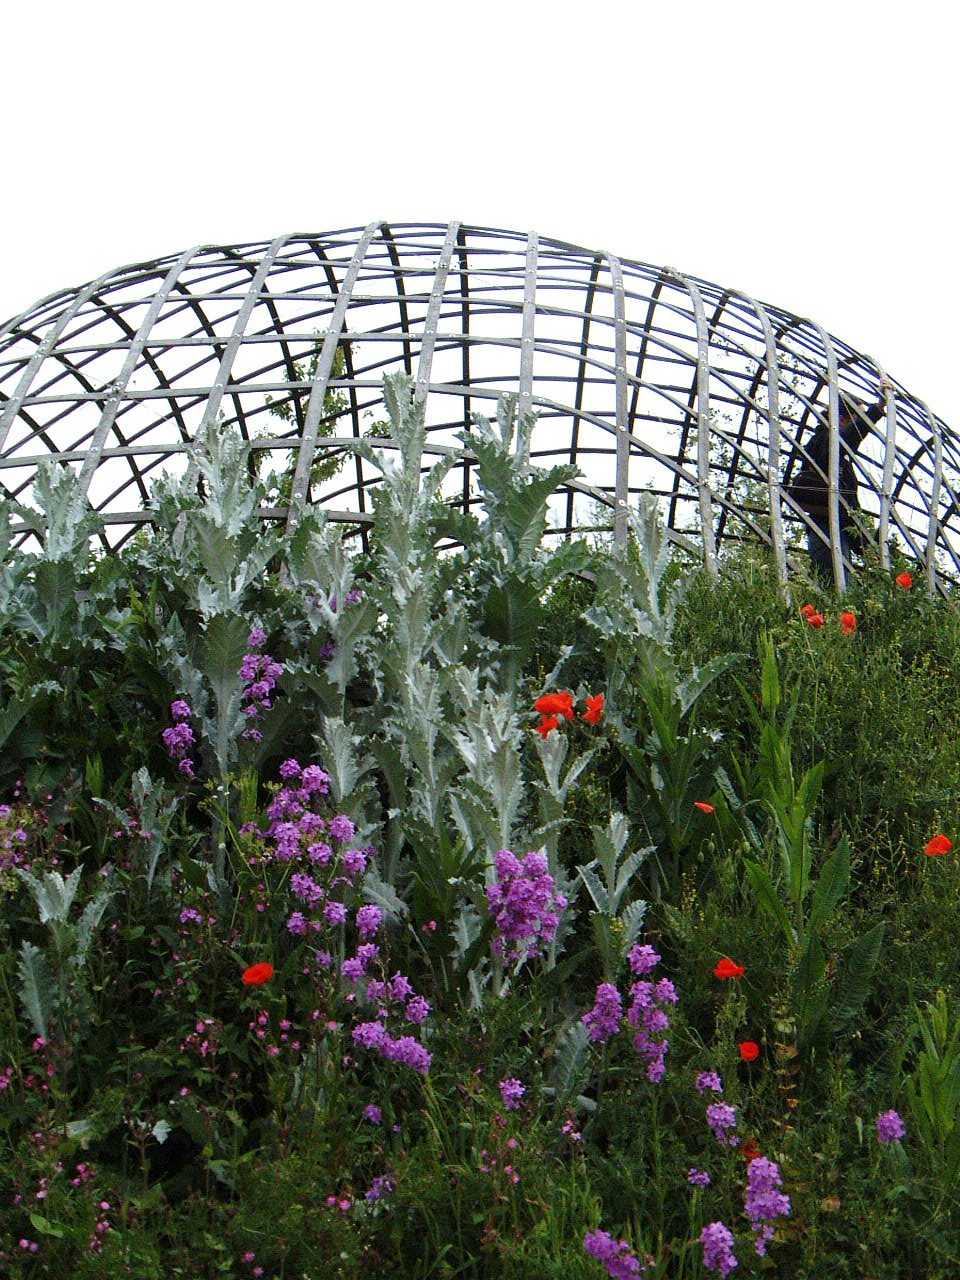
\includegraphics[width=0.48\textwidth]{doncaster_ext.jpg}\label{fig:doncaster_b}}
		%
		\vspace{10pt}
		\captionof{figure}[Timber gridshells built in 1998 in Doncaster, England]{Timber gridshells built in 1998 in Doncaster, England}
		\label{fig:doncaster}    
\end{figure}

These projects definitely trailed the technique in England and initiated the renewal period (see \cref{sec:renewal}). Although they remained small-scale projects for which modeling was achieved through physical models, they trained and restored partially the operational ability of Buro Happold to design timber gridshells as pointed by \citet{Harris2003}.

\subsection{The renewal : Hannover, Downland and Savill}
\label{sec:renewal}

What was missing for elastic gridshells to re-emerge after the major experiment of Mannheim was probably the development of modern numeric tools to ease and speed up the design process.\footnote{\blockcquote[]{Harris2003}{The key to the modern use of timber gridshells is the development of computer methods in modelling complex three-dimensional shell structures. For the Mannheim structure, the primary method of form finding was the use of physical models. The Earth Centre structures were small and easily modelled using wire mesh, but when Buro Happold were commissioned to design the Japanese Pavilion for Expo 2000 in Hannover (Architect Shigeru Ban), it was apparent that much more sophisticated computer form finding and analysis would be necessary.}} Amongst those tools we should identify two main categories~: geometry processing softwares and structural analysis softwares. Recall that in the 70's, geometry processing was done through physical models and photographic measurements \cite[pp.~130-135]{IL10} while structural analysis was conducted through a compound of physical model testing with scaling techniques \cite[pp.~130-135]{IL13}, hand calculations and the very first numerical formfinding calculations \cite[pp.~184-193]{IL10} and finite element calculations \cite[pp.~210-217]{IL10}.

In the late 90's, the rise in importance of computer methods offered new possibilities.

\subsubsection{Japan Pavilion, Hannover, Germany, 2000}
In 1997, architecte Shigeru Ban began to collaborate with Frei Otto and Buro Happold to design the \emph{Japan Pavilion} for \emph{Expo 2000} in Hannover, Germany \cite{Ban2006}. This pavilion was a large-scale corrugated gridshell made out of cardboard tubes, about 75 meters long and 25 meters wide. Corrugations bring curvature, and therefore enhance the strength of the shell. The tubes were tied together with a fabric tape, a very low-tech joint (see \cref{fig:hannover_a}). The structure was covered with a paper membrane specially developed for the project to meet the requirements of the german fire regulations (see \cref{fig:hannover_b}). For the occasion, a new erection method was set up in which the grid was laid out not at the ground level but at a higher level on a hydraulic scaffold platform. From there, the grid was pushed up into position using the platform's jacks. It was found late that the cardboard tubes were subject to a high level of creep. This required the introduction of new timber arches to reinforce the gridshell and to enlarge the existing timber rafters intended to brace the grid and support the paper membrane (see \cref{fig:hannover_a}).
\begin{figure}[t]
		\subfloat[][Interior view]{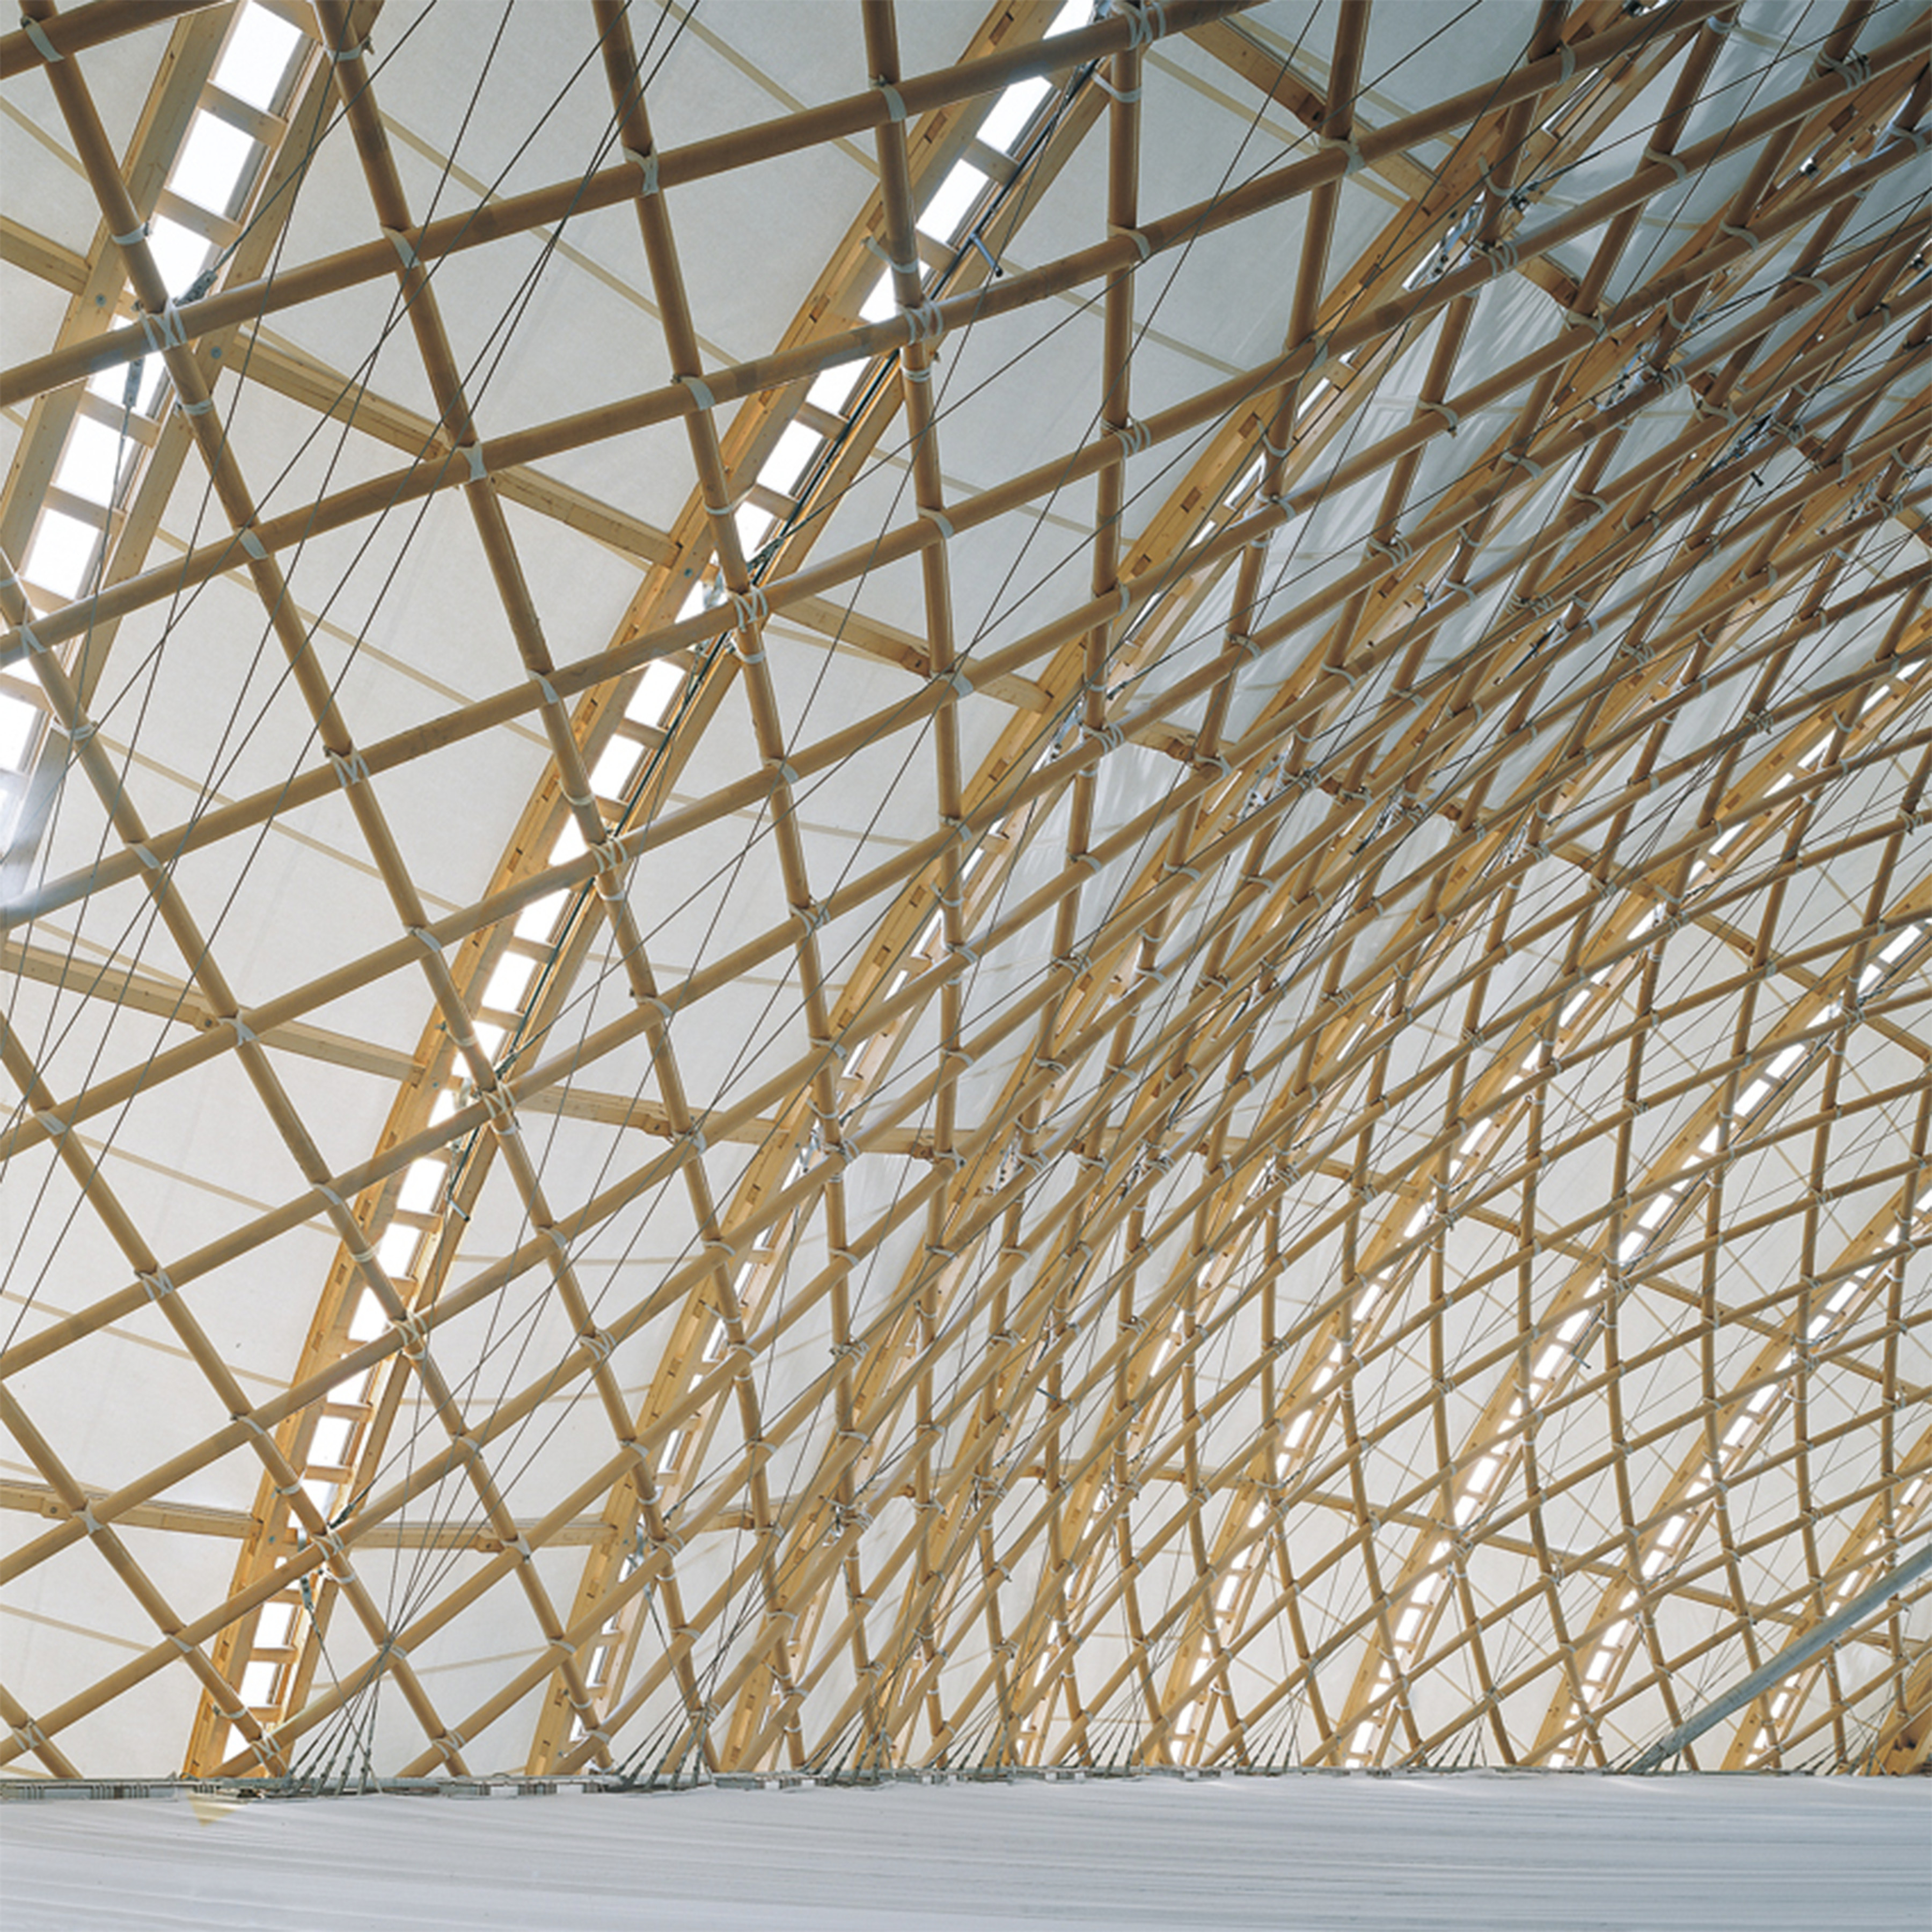
\includegraphics[width=0.32\textwidth]{hannover_int.jpg}\label{fig:hannover_a}}
		\hspace*{\fill}
		\subfloat[][Sky view]{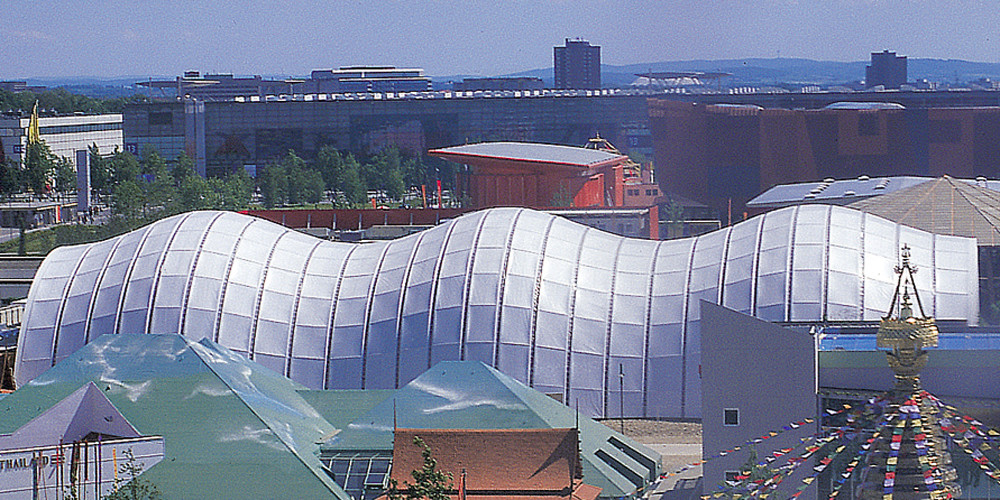
\includegraphics[width=0.64\textwidth]{hannover_sky.jpg}\label{fig:hannover_b}}
		%
		\vspace{10pt}
		\captionof{figure}[Carboard gridshell built for Expo 2000 in Hannover, Germany]{Carboard gridshell built for Expo 2000 in Hannover, Germany.}
		\label{fig:hannover}    
\end{figure}

\subsubsection{Weald and Downland, Downland, England, 2002}
The design of the \emph{Downland} gridshell began right after the completion of the Westminster Lodge (see \cref{sec:signs}) where architects from E. Cullinan Studio became acquainted with the enginneers from Buro Happold. At Downland, the project team truly revived the technique of large-scale timber gridshells while bringing lots of improvements to the system. The building opened to the public in 2002. Its corrugated shape recalls the one of the Japan Pavilion from which it was inspired (see \cref{fig:downland_b}).

The building is 50 meters long and 12.5 to 16 meters wide, covering an area of about \SI{675}{m^2} for a height varying from 7 to 9.5 meters \cite{Harris2002}. The structure is a double-layer gridshell made of rectangular oak laths of cross-section \SI{50}{mm} x \SI{35}{mm} (see \cref{fig:downland_a}). To produce high grade timber elements, the continuous laths were re-formed from small carefully selected wood pieces, finger-jointed every \SI{60}{cm} in \SI{6.0}{m} length pieces. These pieces of lath were then scarf-jointed on site every \SI{6}{m} to obtained the desired length, up to \SI{50}{m}.

The grid pitch is \SI{1.0}{m} except in weaker areas where it is \SI{0.5}{m}. There, the grid is twice denser to achieve the required buckling resistance \cite{Harris2003}. Rib-lath bracing was preferred to steel cable bracing as ribs were deemed to offer a more convenient support for the cladding elements and to reduce the complexity of the connection. A new connection system was developed to avoid the cost of drilling thousands of slotted holes that would, in addition, reduce the cross-section area, while maintaining the required scissor behavior for the deformation of the timber lattice.\footnote{This detail was \href{https://patents.google.com/patent/GB2361504A/en?q=\%22A+coupling+and+a+method+of+constructing+grid+shell+buildings+using+such+a+coupling\%22&country=GB}{patented} by the design team and the client.}
 \begin{figure}[t]
		\subfloat[][Interior view]{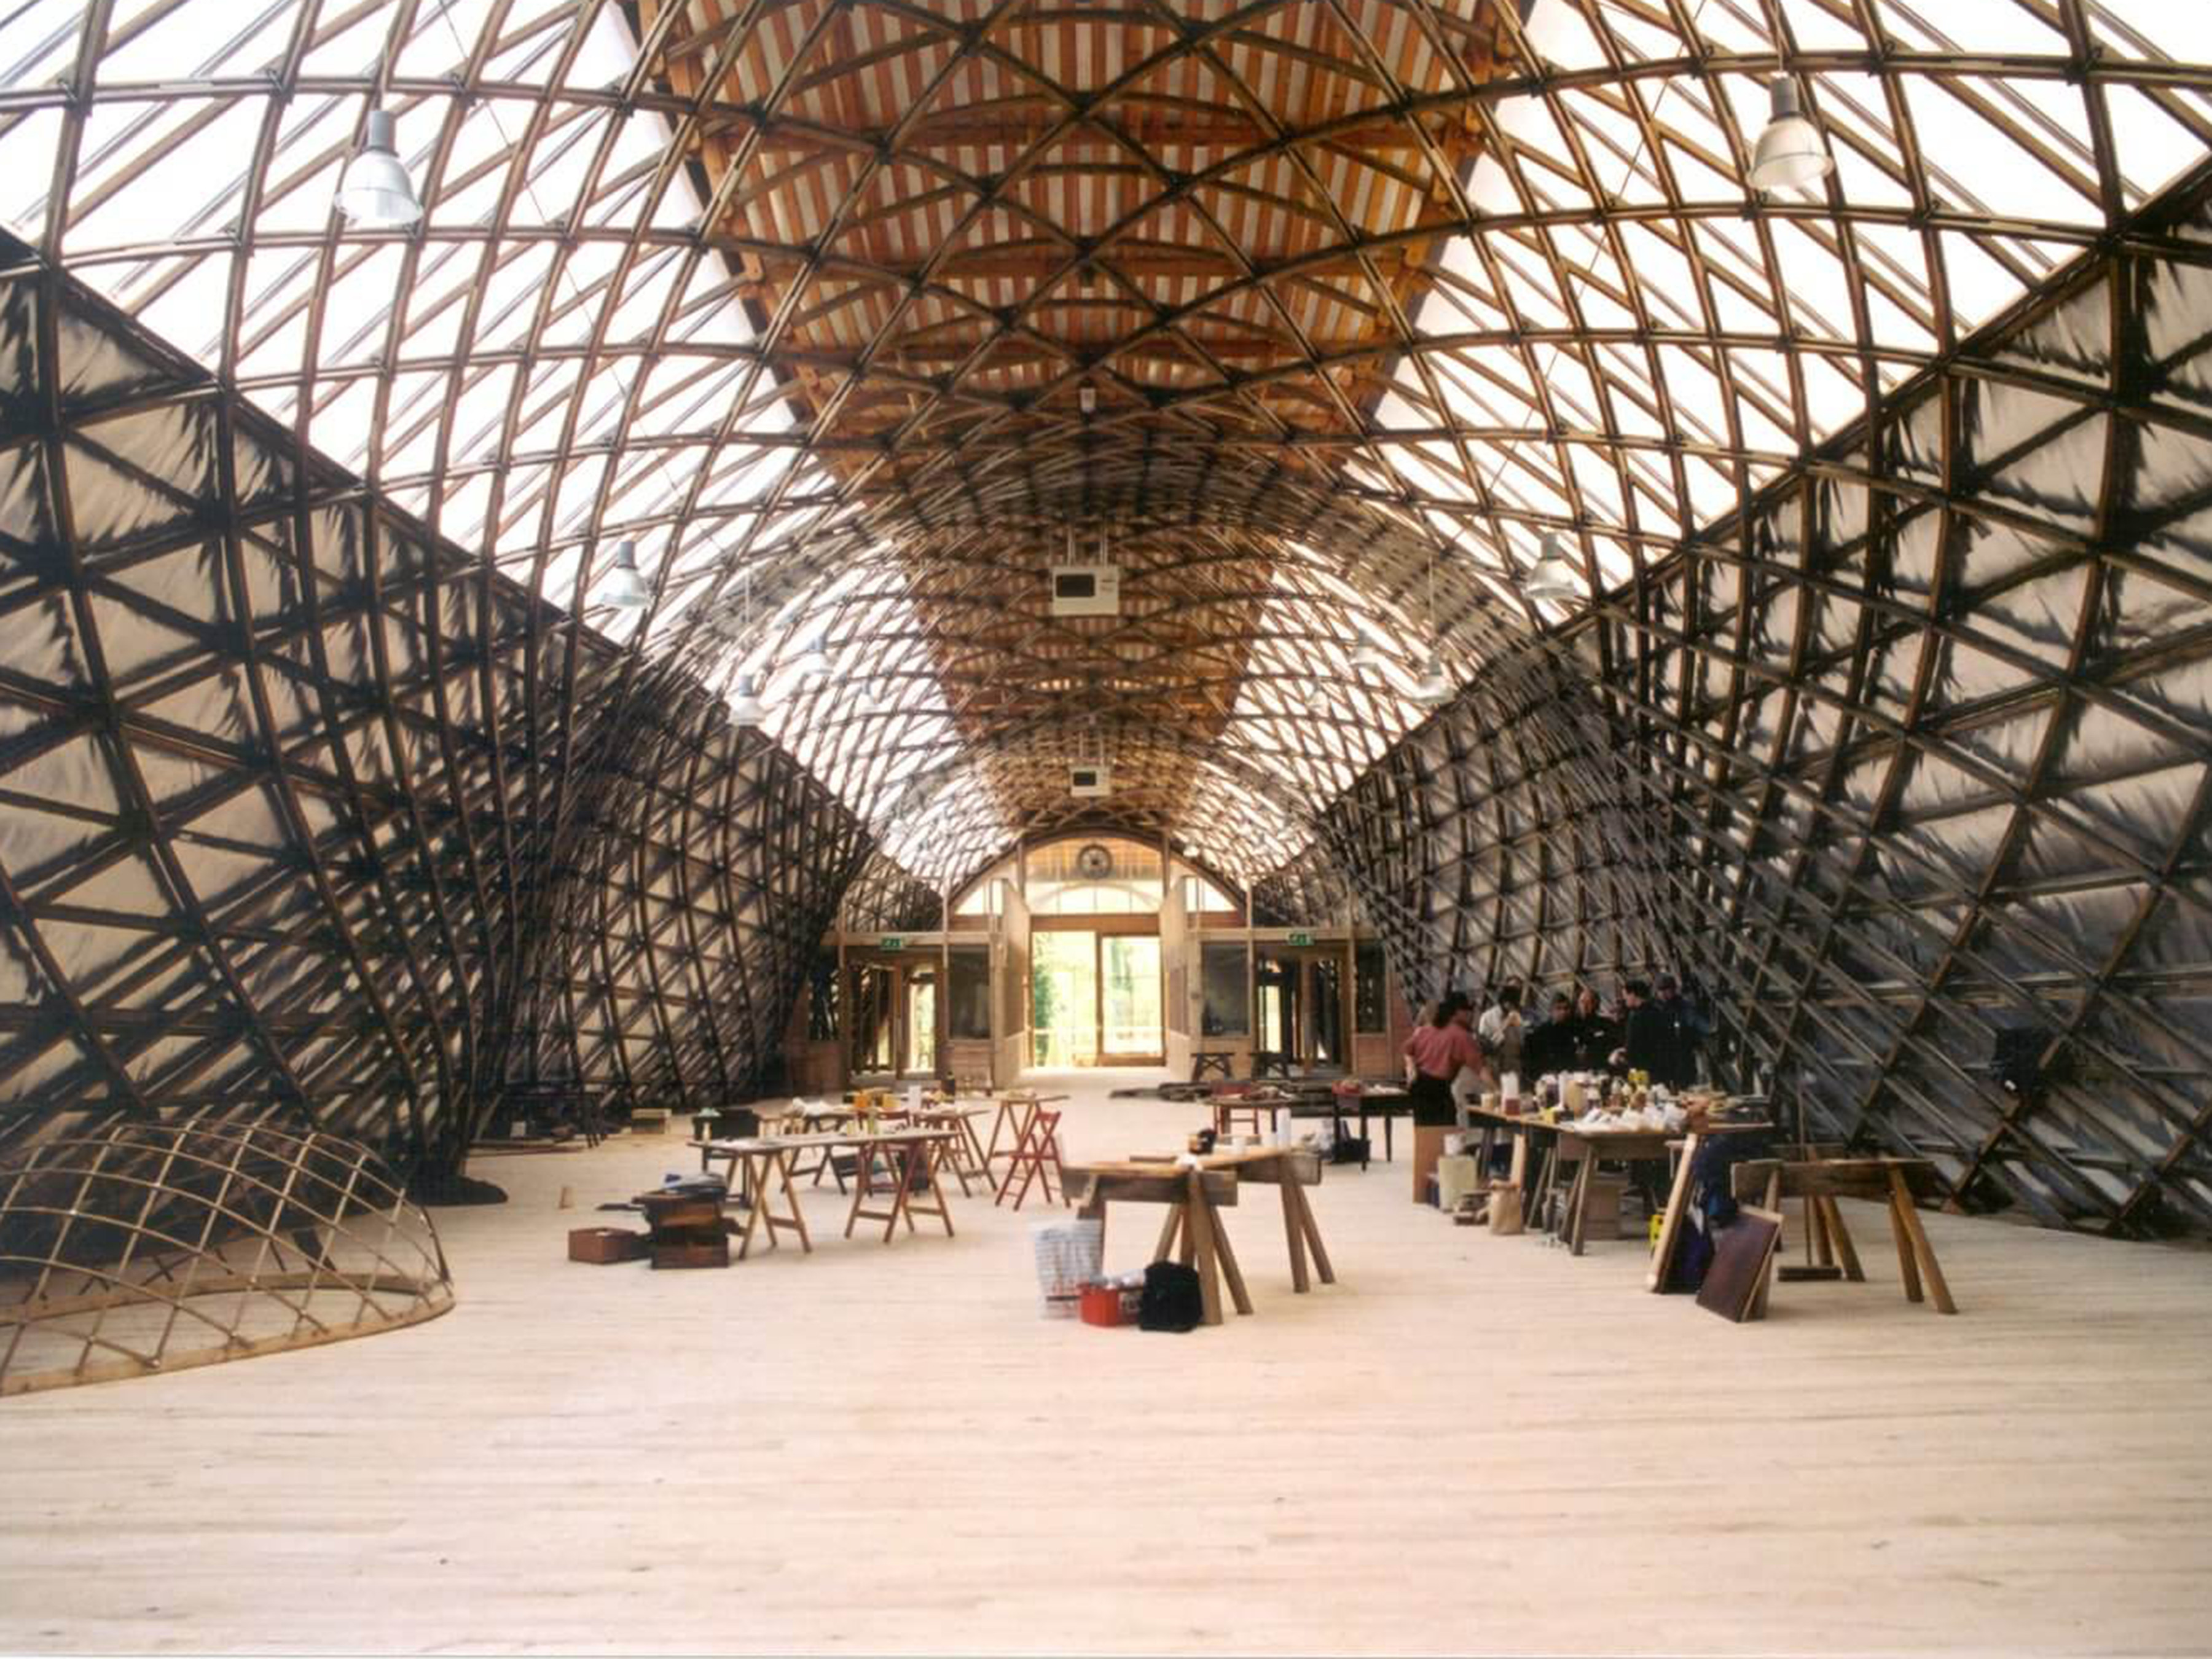
\includegraphics[width=0.48\textwidth]{downland_b.jpg}\label{fig:downland_a}}
		\hspace*{\fill}
		\subfloat[][Exterior view]{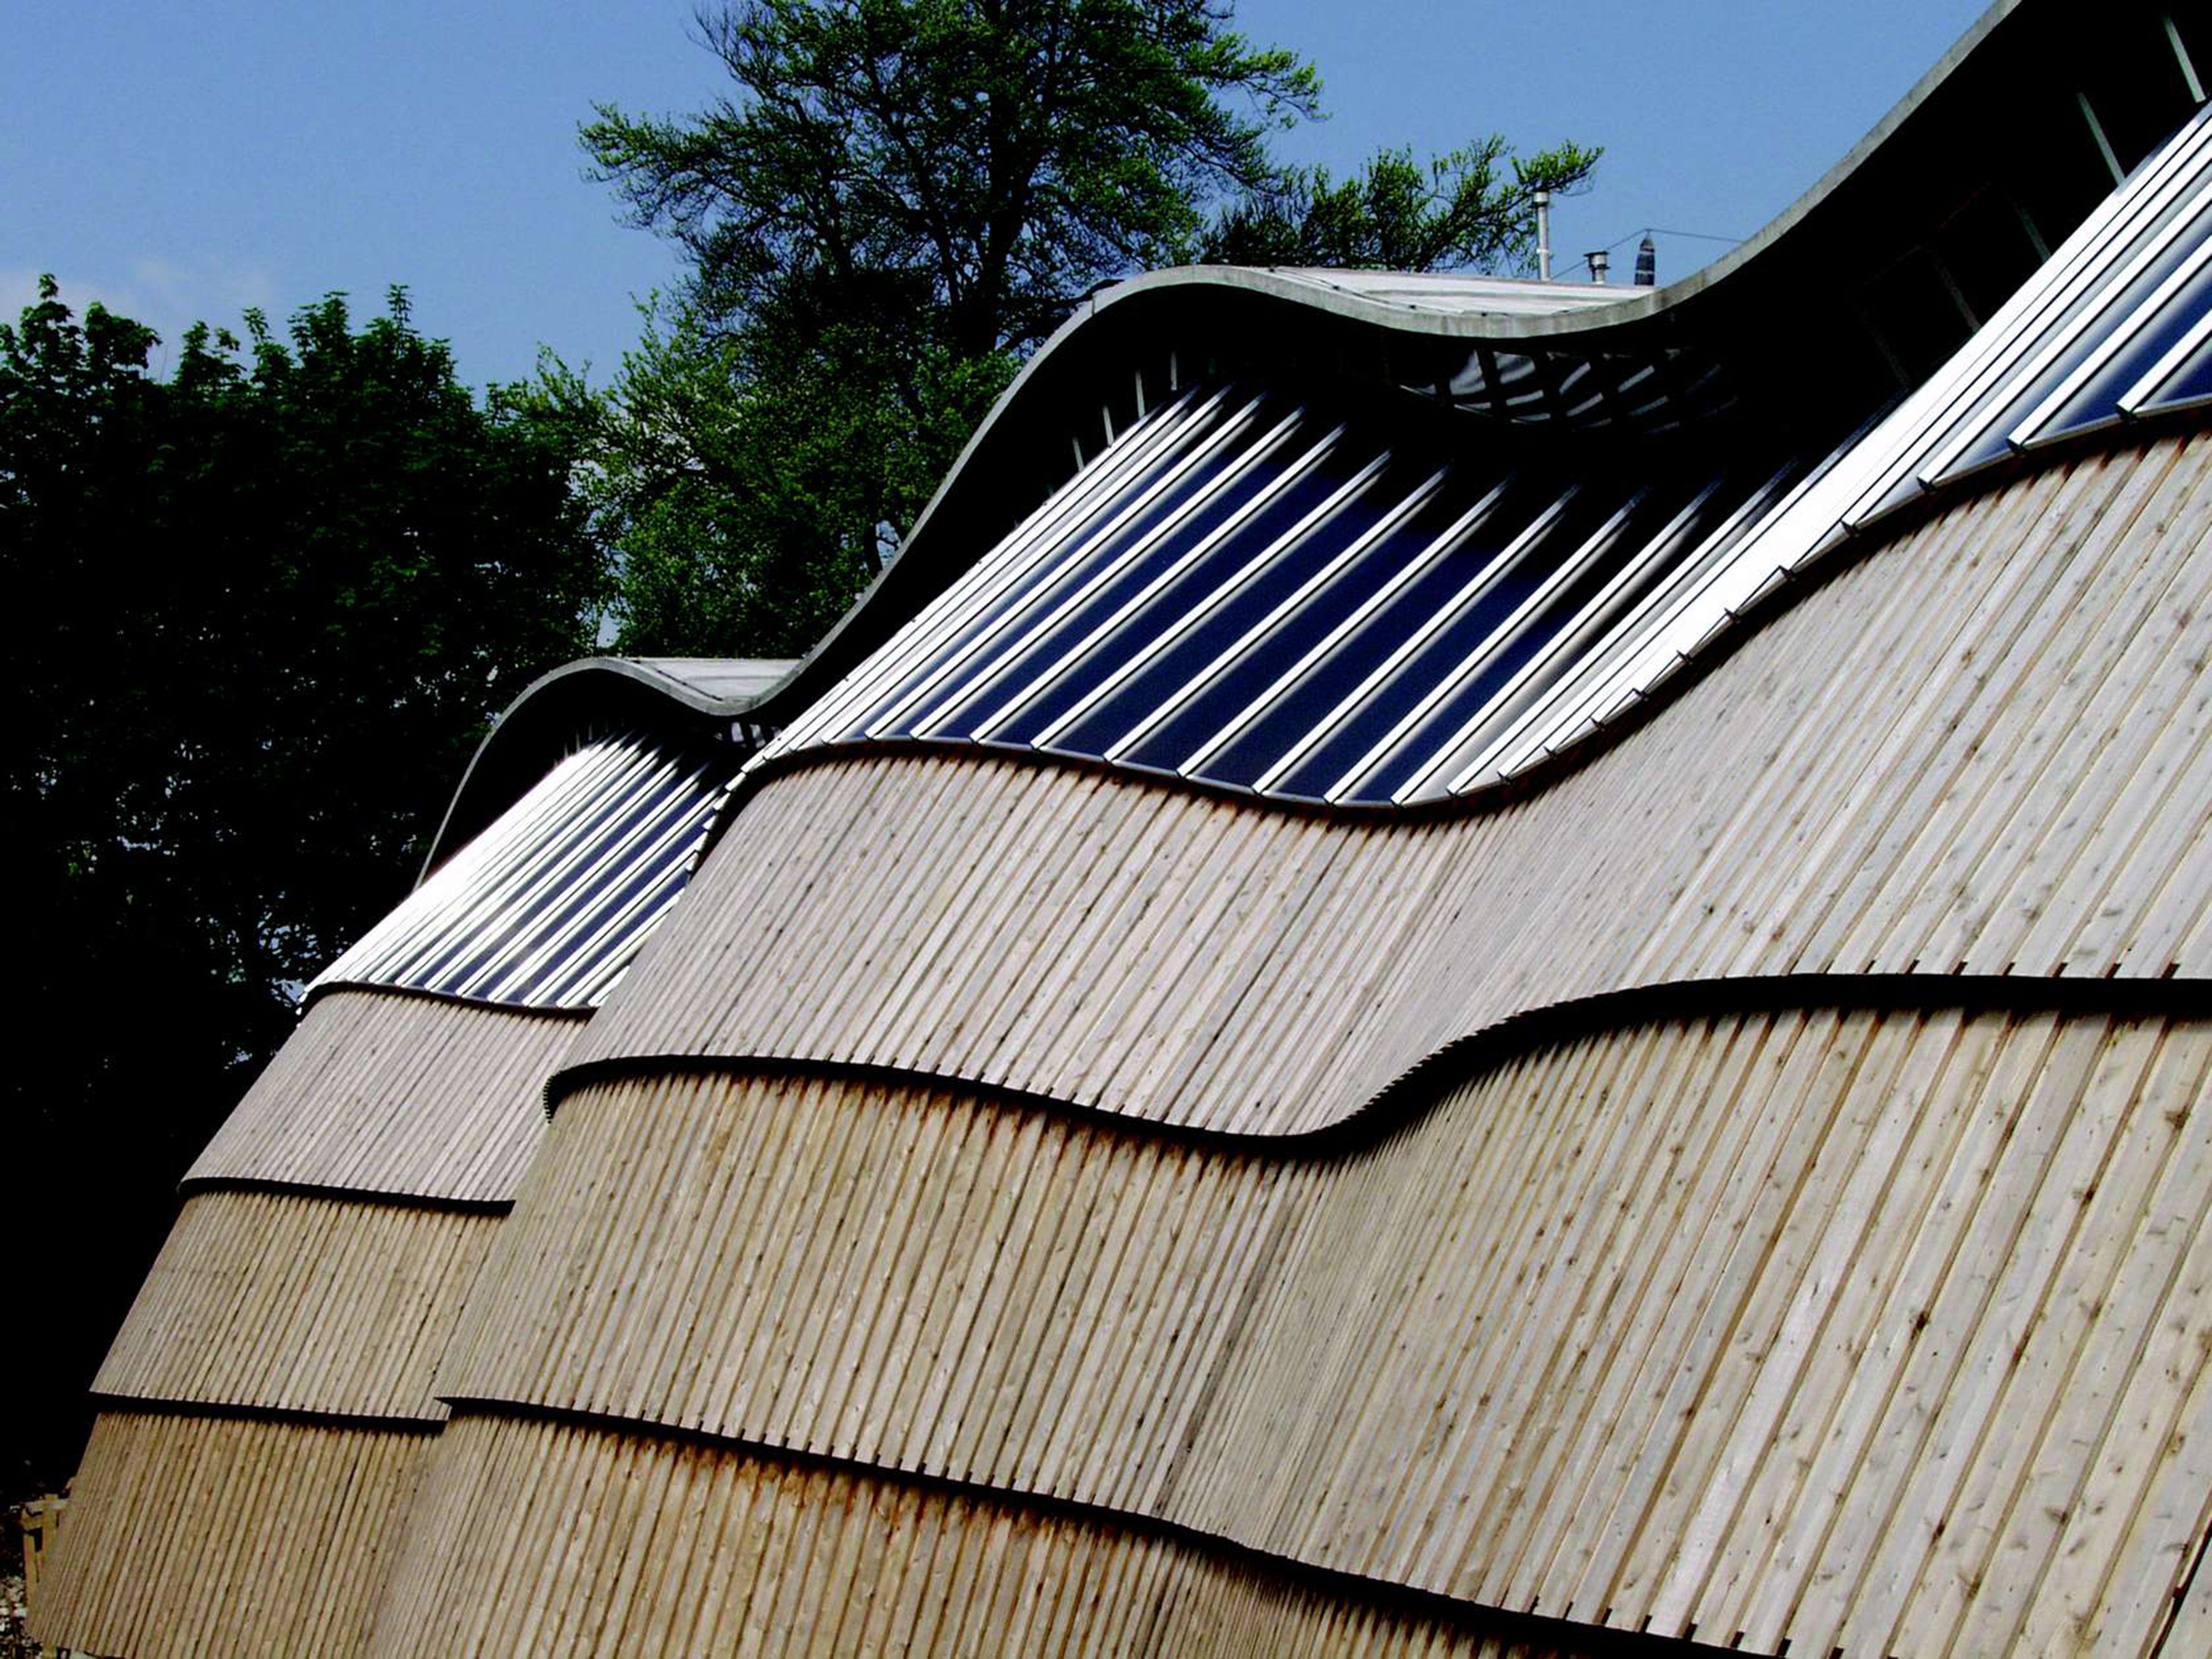
\includegraphics[width=0.48\textwidth]{downland_a.jpg}\label{fig:downland_b}}
		\vspace{10pt}
		\captionof{figure}[Timber gridshell built in 2003 in Downland, England]{Timber gridshell built in 2003 in Downland, England.}
		\label{fig:downland} 
\end{figure}

The flat lattice was laid out on a scaffold platform. Unlike the Japan Pavilion, the lattice was progressively lowered down into position. This stage took 6 weeks. Once deformed, the shear blocks were introduced in the grid and bracing rib-laths were installed, giving its full strength to the shell. Finally the gridshell was cladded with a mix of polycarbonate plates (to let the light in) and timber boards on top of insulation panels and a rain screen.

It is worth to mentionne that for the first time the form was not found by inverting some sort of hanging chain model that would produce a pure funicular shape where only compression occurred. Instead, the shape was the result of a numerical computation that took into account the bending behavior of the laths.\footnote{This software was developed by Chris Williams of the University of Bath.} \citet{Harris2003} argued that computer models enabled some interactivity in the formfinding process that would not be possible with physical models, leading to a better synergy between architectural and structural requirements. They also argued that physical models contributed invaluably to the development of a creative and efficient design throughout the project.

\subsubsection{Lothian Gridshell, Pishwanton, England, 2002}
This project deserves somme attention because the developed approach was completely different from the projects exposed until now~: \blockcquote[]{Lowenstein2002}{Previous projects have portrayed the method as a highly technical use of a low tech resource. This, however, need not be the case as we see with this project \belp{}}. The structure was the result of~: \blockcquote[]{bdonline2002}{\belp{} an unusual collaboration between sole practitioner Christopher Day, engineer David Tasker, a crowd of local volunteers and (more unusually) the philosophies of Rudolf Steiner and Johann Wolfgang Goethe}.\footnote{From the online paper \textquote{The other gridshell} : \url{http://www.bdonline.co.uk/the-other-gridshell/1020435.article}}.
 \begin{figure}[h]
		\subfloat[][Interior view]{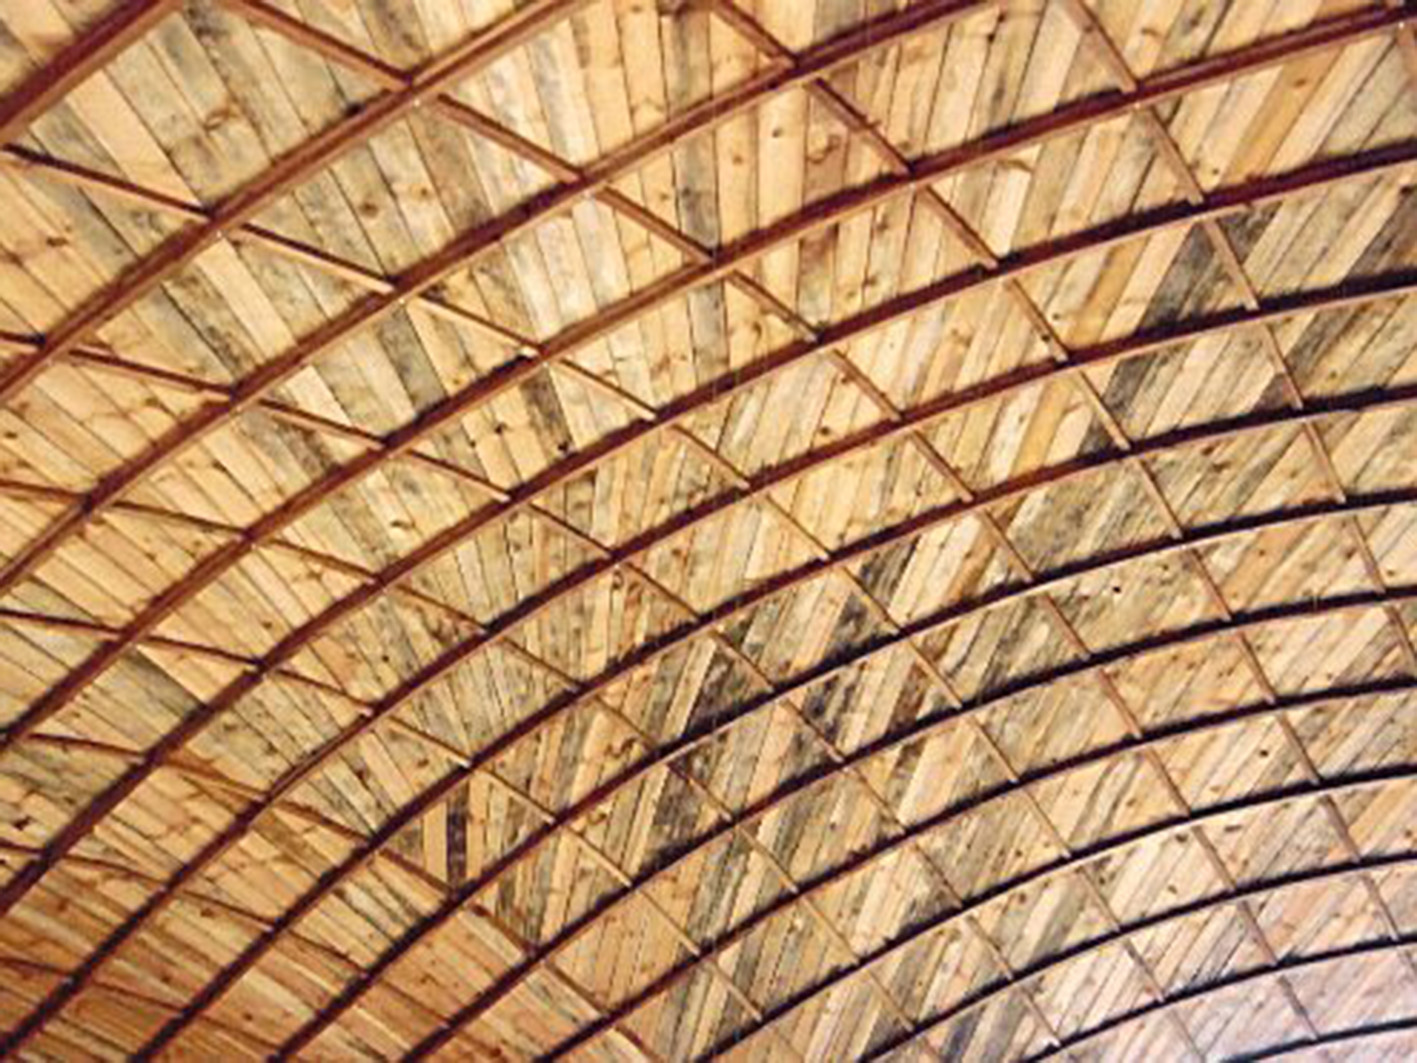
\includegraphics[width=0.48\textwidth]{pishwanton_int.jpg}\label{fig:pishwanton_a}}
		\hspace*{\fill}
		\subfloat[][Exterior view]{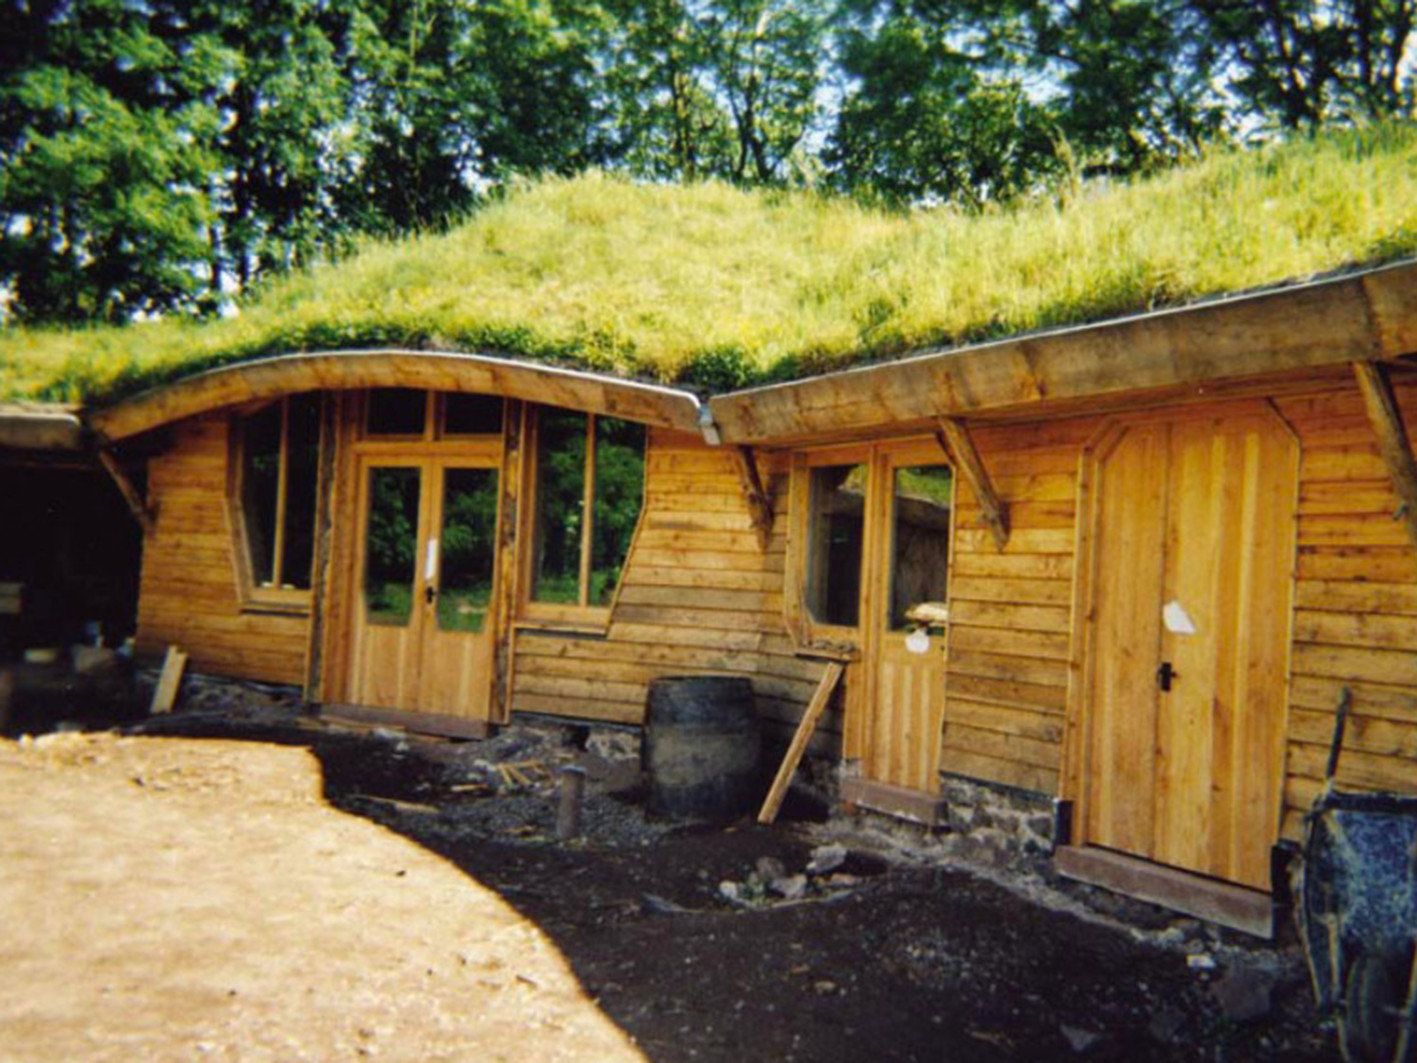
\includegraphics[width=0.48\textwidth]{pishwanton_ext.jpg}\label{fig:pishwanton_b}}
		\vspace{10pt}
		\captionof{figure}[Timber gridshell built in 2002 in Pishwanton, England]{Timber gridshell built in 2002 in Pishwanton, England.}
		\label{fig:pishwanton} 
\end{figure}

The single-layer gridshell was made out of local larch. Once erected by hands, the dome-like shape covered about \SI{80}{m^2} and spanned 10 meters. The grid was braced with timber boards (see \cref{fig:pishwanton_a}) and covered with a planted turf roof (see \cref{fig:pishwanton_b}). Some calculations were made but in the end, it had to carry load testing to prove its safety and gaine its regulation approval.\footnote{\blockcquote[]{bdonline2002}{There were a lot of calculations but no computer-generated models to show they all added up. In fact, the form was previously established with scale models. When it came to gaining Building Regulations approval, the team needed to prove that the building would be strong enough. So Tasker arranged for the unfinished structure to be loaded with about 18 tonnes of sand from a local quarry – equivalent to the maximum predicted snow load, plus a safety factor.}}

\subsubsection{Woodland Centre, Filmwell, England, 2003}
The gridshell of the Woodland Center was built 7 years after the project had started.\footnote{More to be found at : \href{http://www.fourthdoor.org/annular/?page_id=441}{Growing and making Flimwell’s chestnut gridshell}.} The building was designed by architecte Feilden Clegg and engineers from Atelier One. It was part of a larger research and development project that aimed at developing chestnut -- a low grad wood -- as a construction material.\footnote{This projet was conducted by the \href{http://www.bre.co.uk/}{Building Research Establishment}.} The building, still existing, is composed of 5 barrel vaults spanning 12 meters and about 5 meters wide. Therefore, it covers about \SI{300}{m^2} \cite{Lowenstein2004}. Each vault module is a transportable unit composed of two curved arches. A single layer gridshell was then applied to this primary frame and braced with chestnut panels. The grid was made of laths with\SI{75}{mm} x \SI{25}{mm} rectangular cross-section, assembled with simple bolts. On top of that, insulation materials and a membrane as rainscreen \cite{FourthDoor2003}.
 \begin{figure}[h]
		\subfloat[][Interior view]{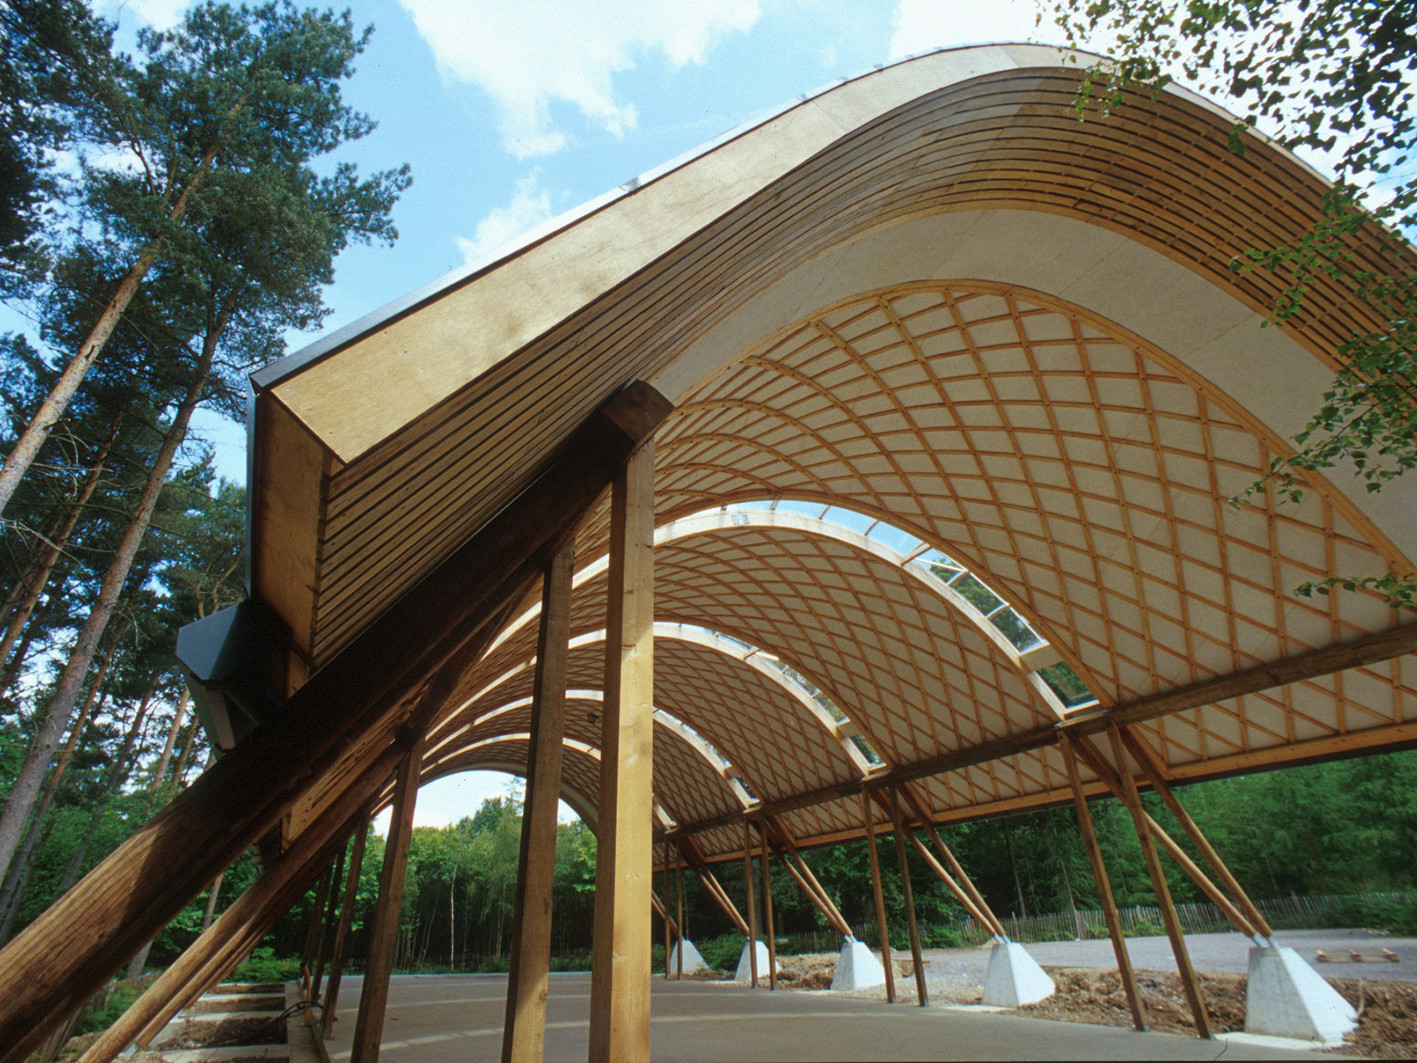
\includegraphics[width=0.48\textwidth]{flimwell_int.jpg}\label{fig:flimwell_a}}
		\hspace*{\fill}
		\subfloat[][Exterior view]{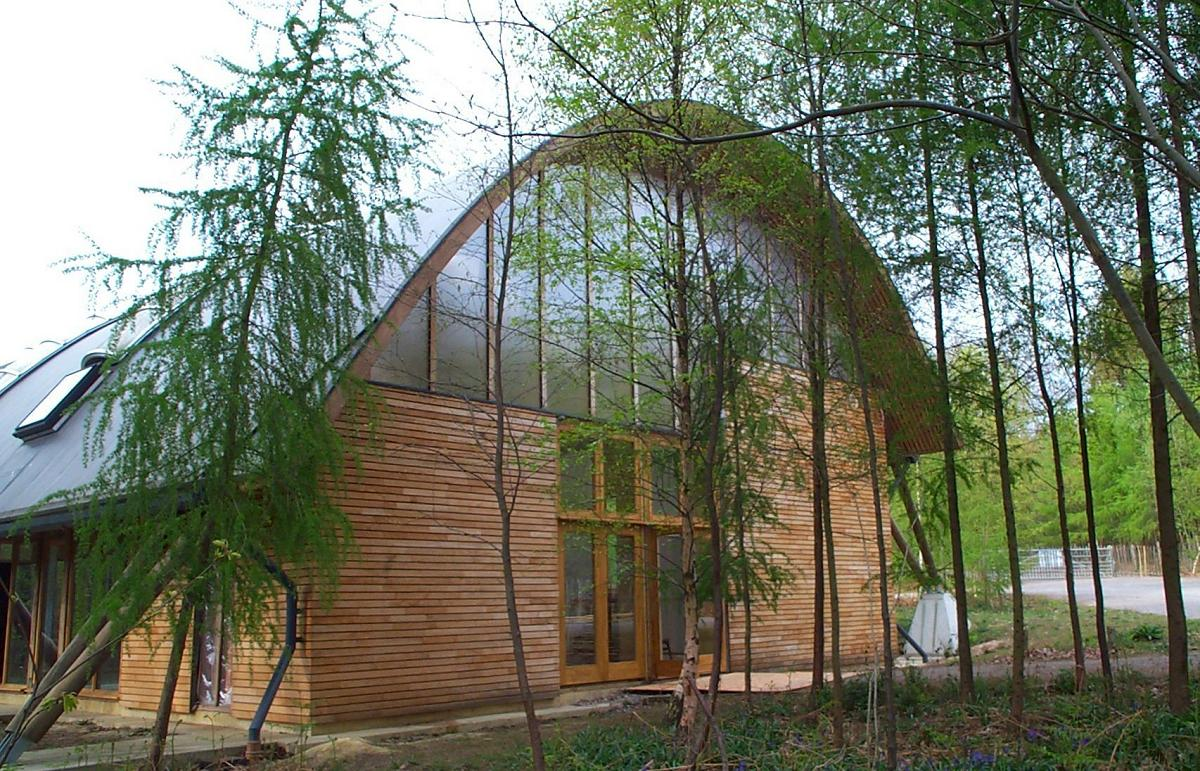
\includegraphics[width=0.48\textwidth]{flimwell_ext.jpg}\label{fig:flimwell_b}}
		\vspace{10pt}
		\captionof{figure}[Timber gridshell built in 2002 in Pishwanton, England]{Timber gridshell built in 2002 in Pishwanton, England.}
		\label{fig:flimwell} 
\end{figure}

\subsubsection{Savill Garden, Savill, England, 2006}

This project saw the light of day thanks to the reputation of the gridshell built in Downland. Again, Buro Happold did the structural design while Green Oak Carpentry realized it. But this time, the architect was Glenn Howells.

The \emph{Savill} gridshell is 90 meters long and 25 meters wide. It covers an area of about \SI{2000}{m^2}, and is therefore almost three times larger than the gridshell in Downland. Once again, the corrugated shape was defined by a parametric equation ($z = f(x,y)$) to enable interactivity between architects and engineers during the formfinding process (see \cref{fig:savill_b}). Chris Williams was responsible for this job.
 \begin{figure}[ht]
		\subfloat[][Interior view]{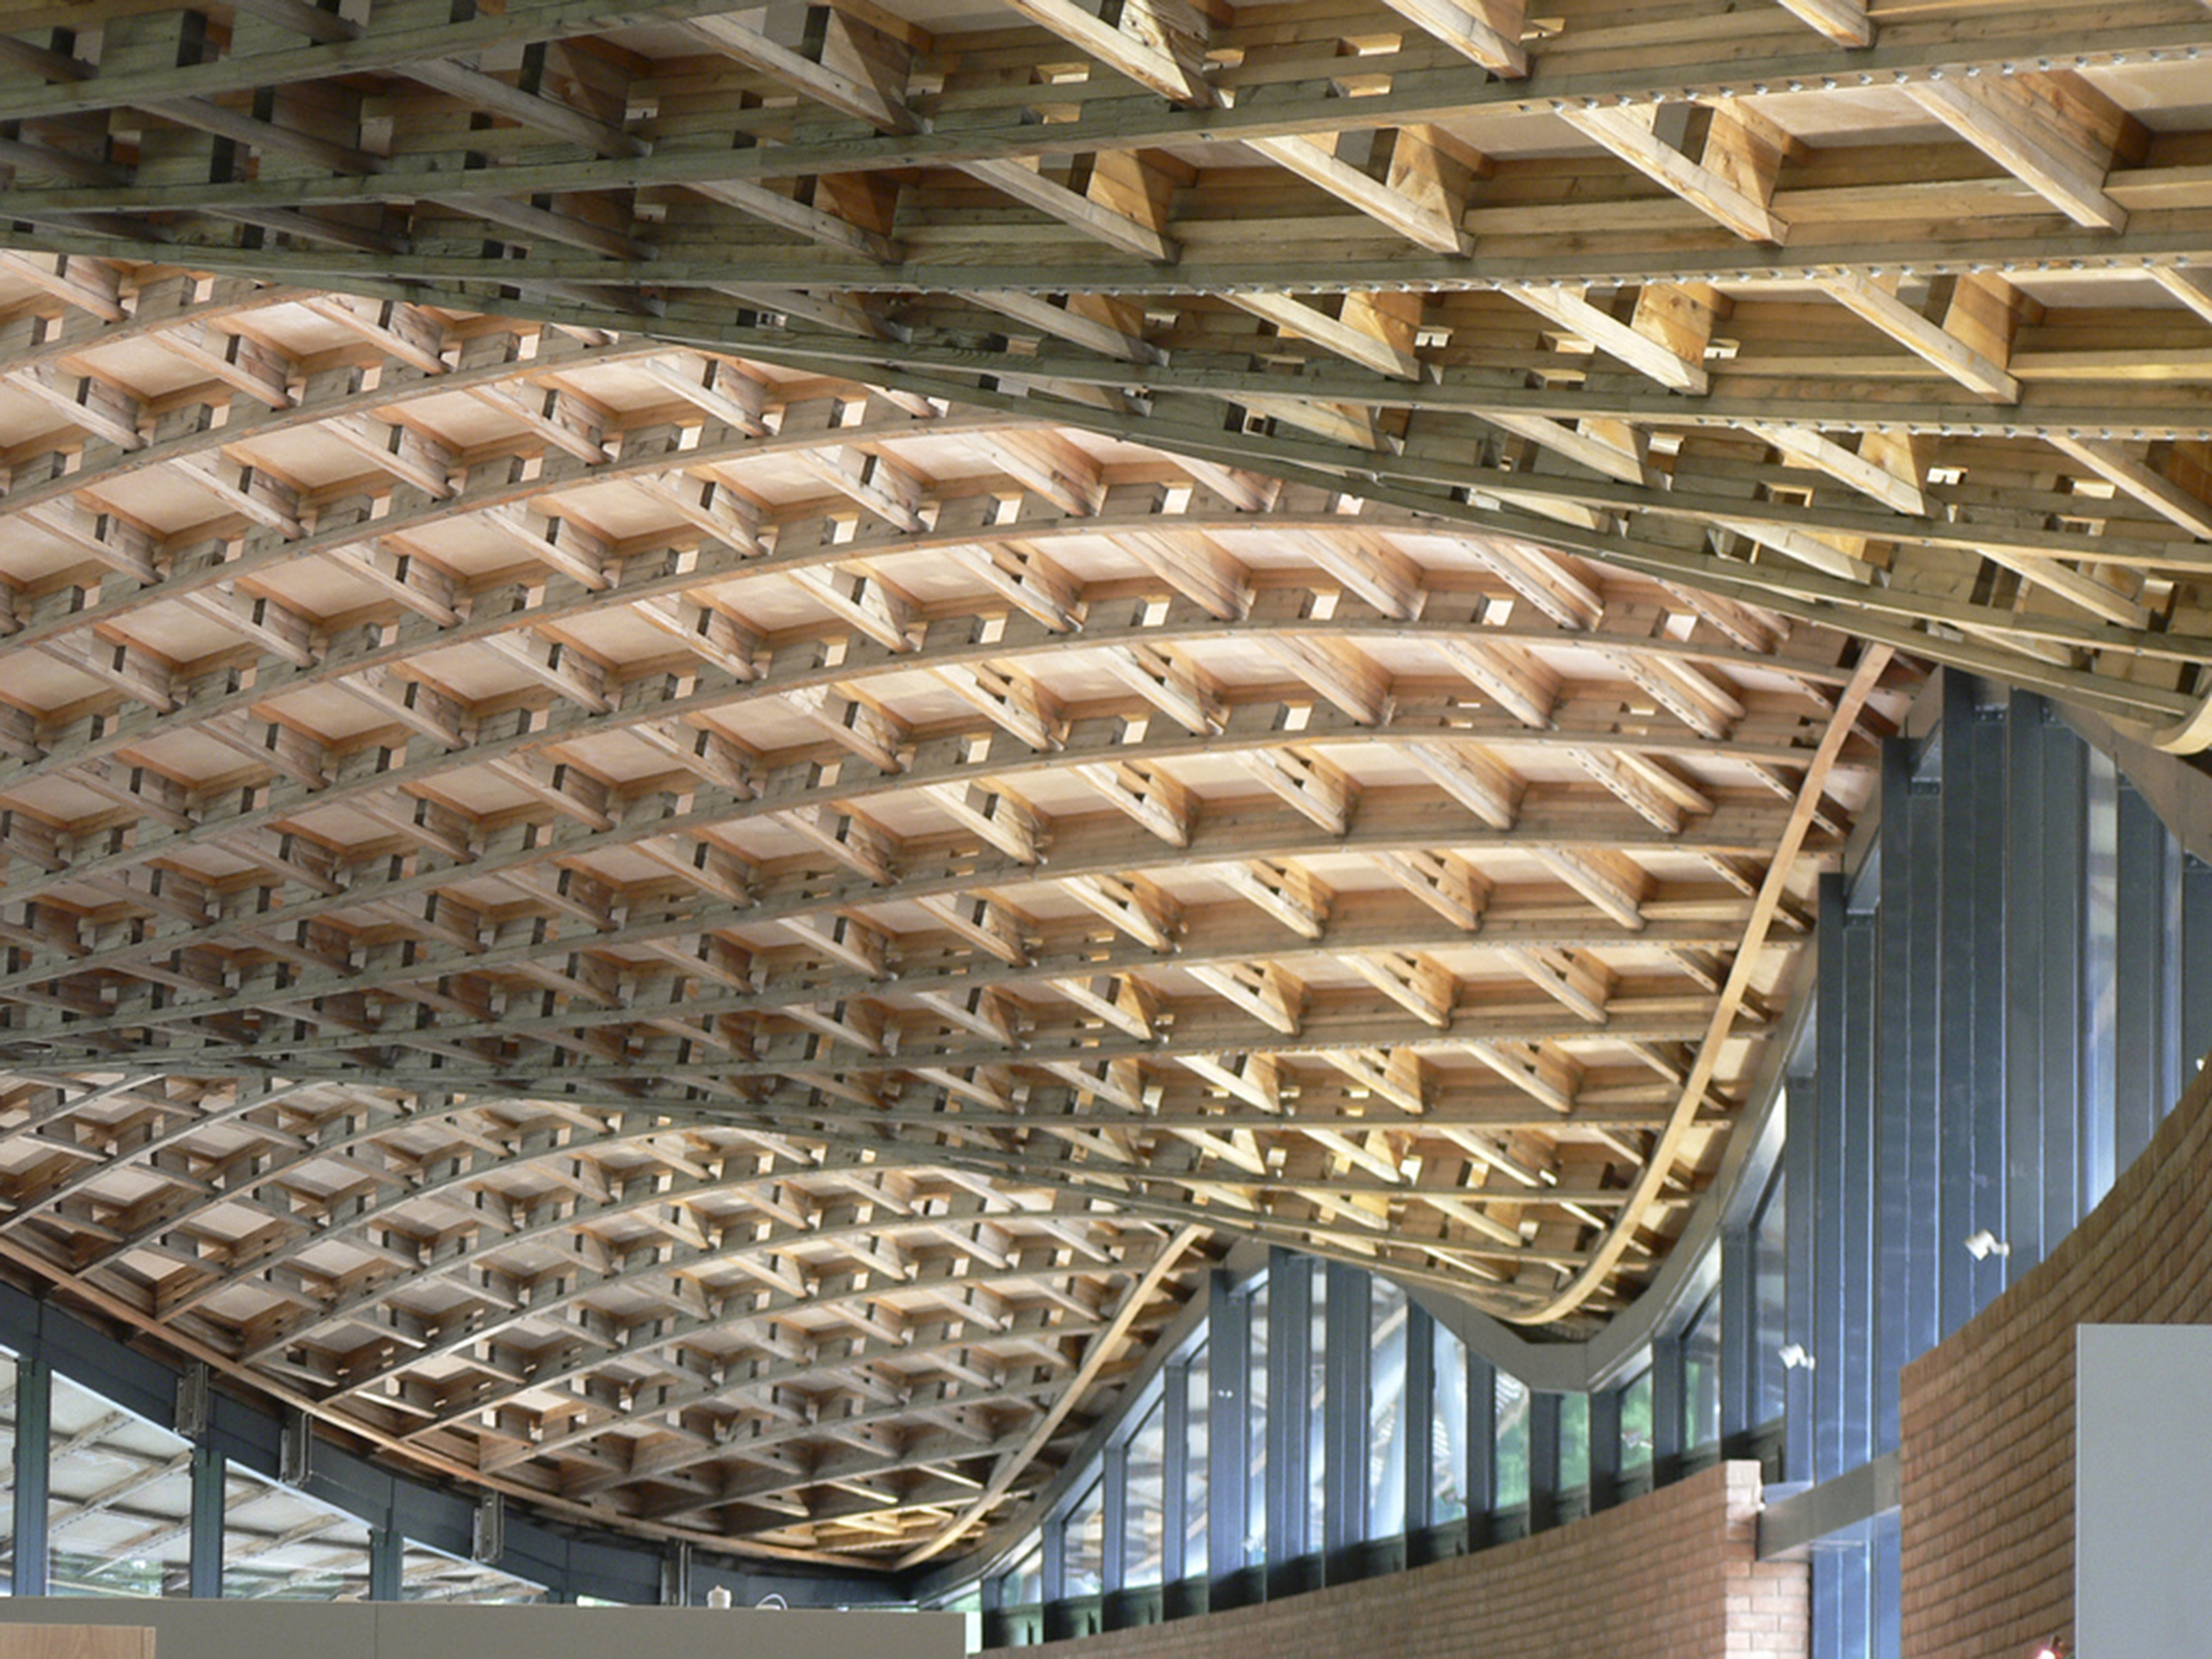
\includegraphics[width=0.48\textwidth]{savill_b.jpg}\label{fig:savill_a}}
		\hspace*{\fill}
		\subfloat[][Exterior view]{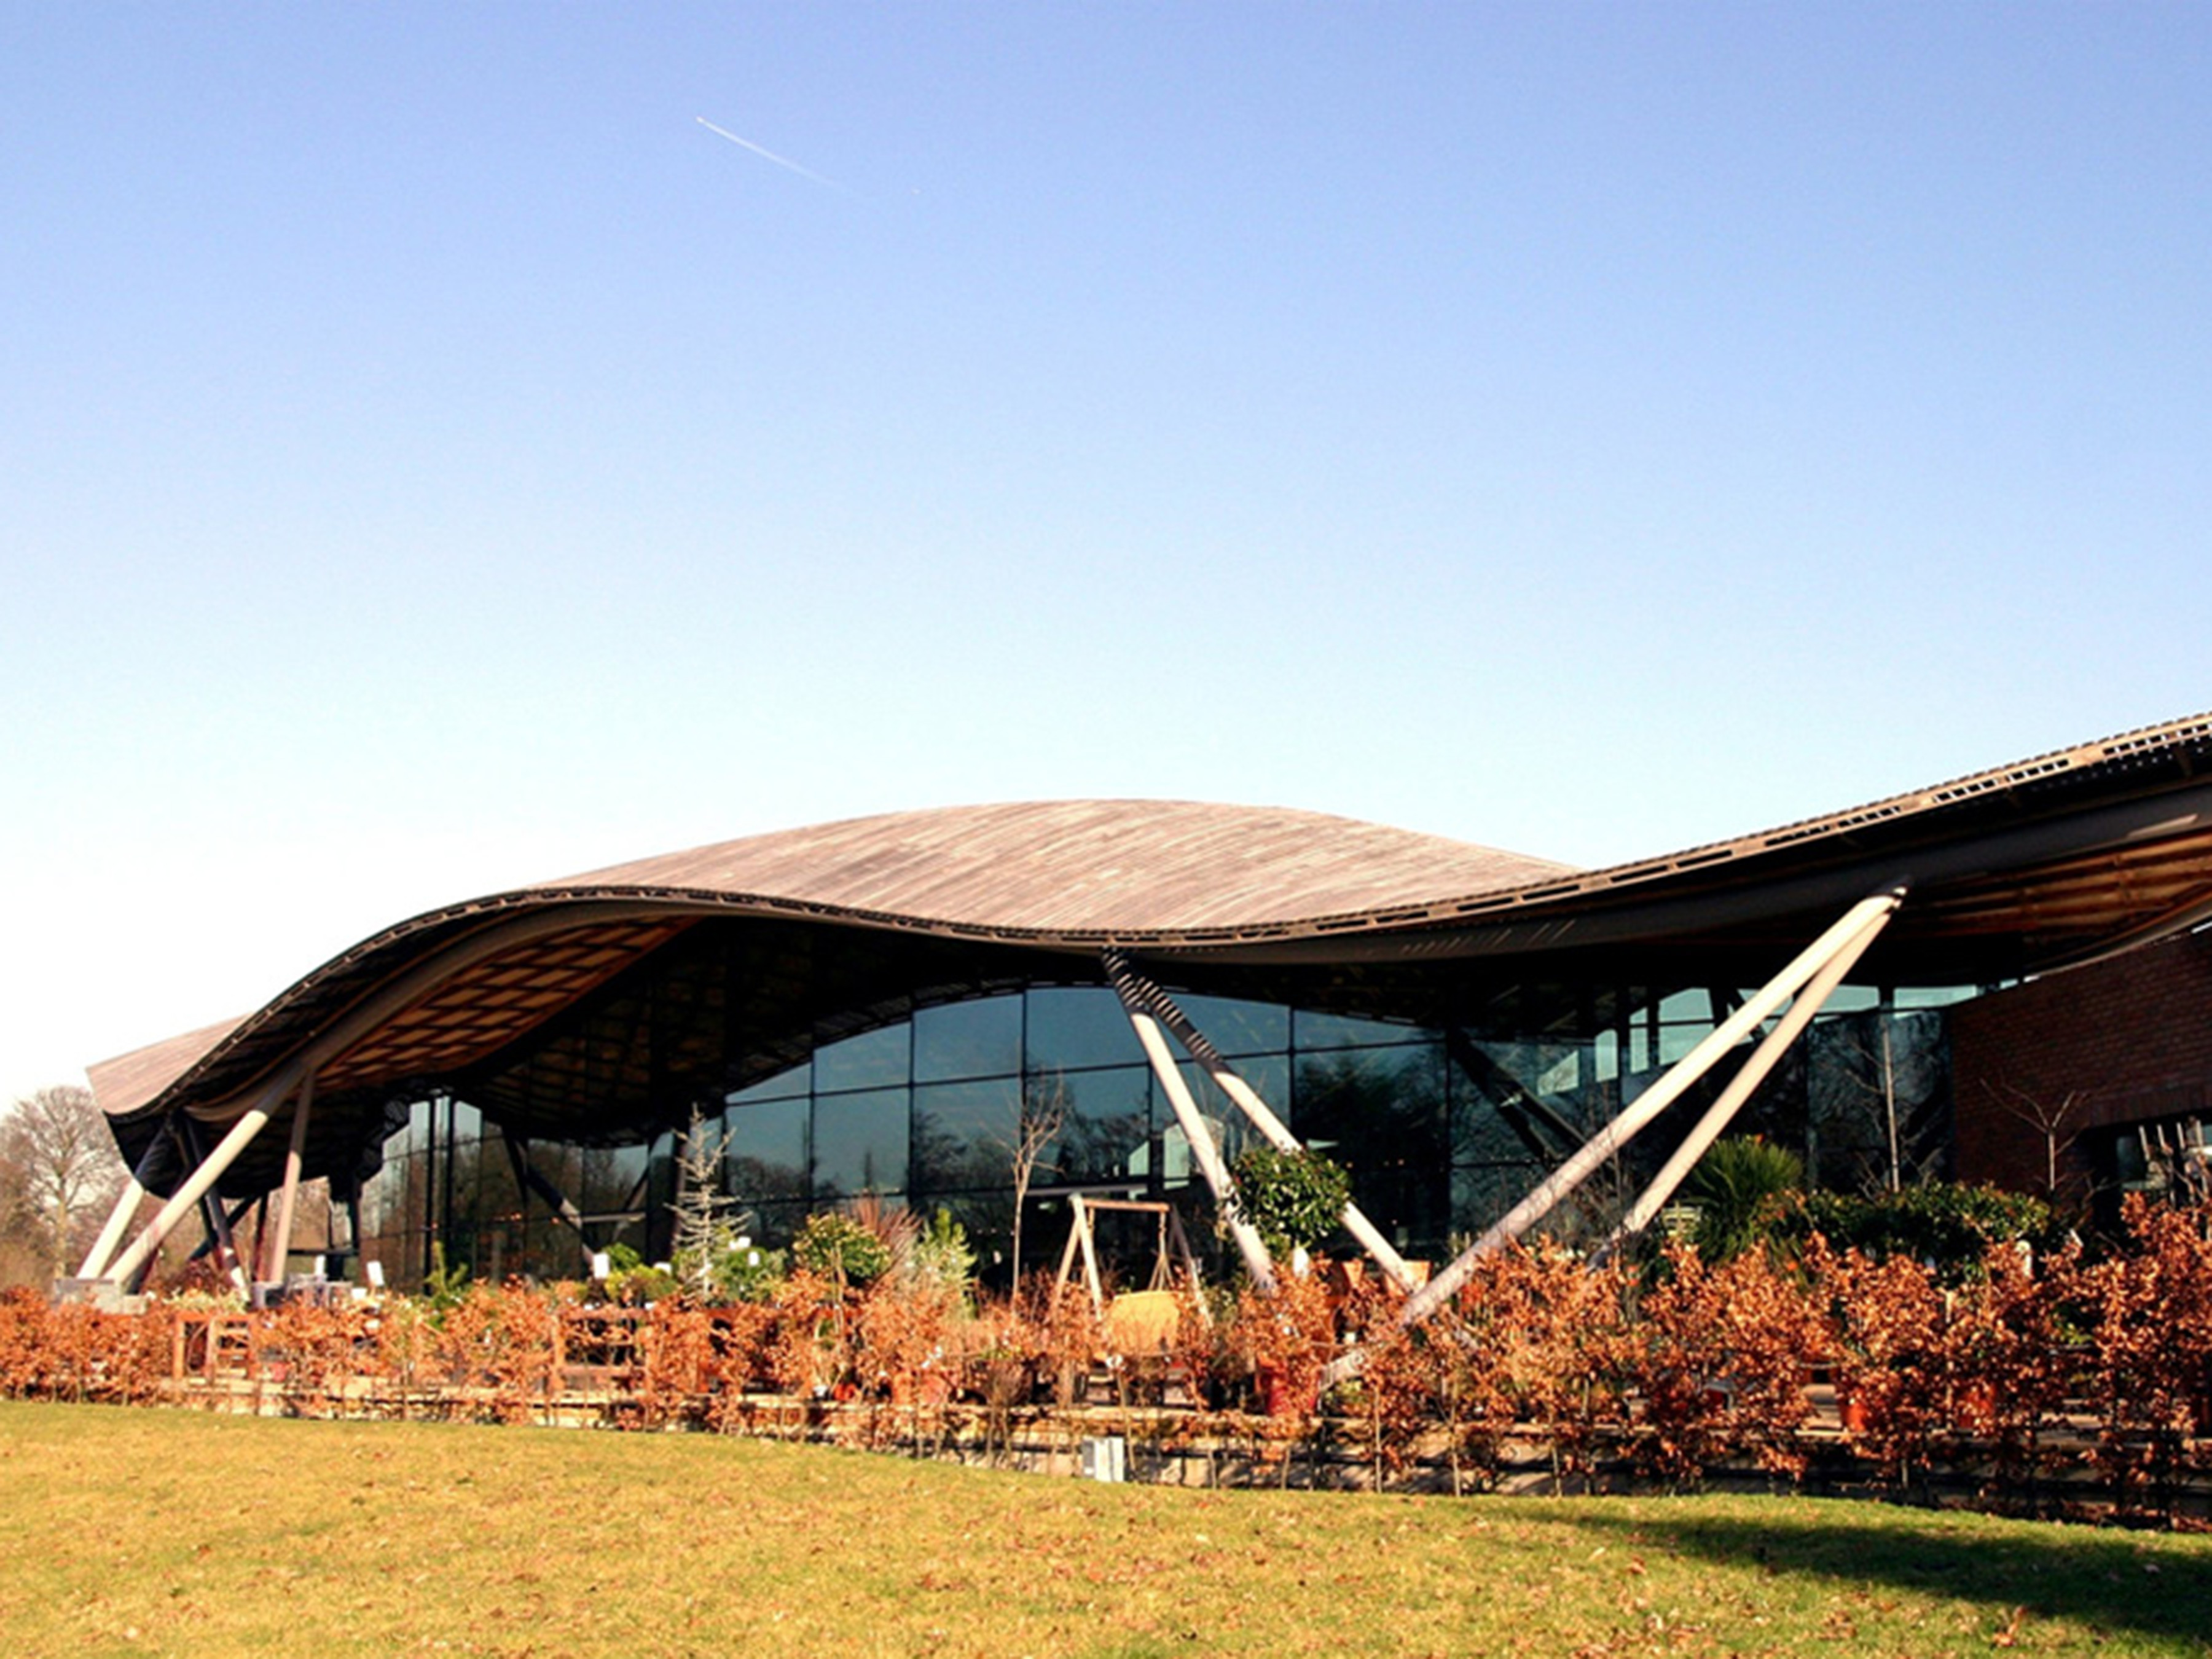
\includegraphics[width=0.48\textwidth]{savill_a.jpg}\label{fig:savill_b}}
		\vspace{10pt}
		\captionof{figure}[Timber gridshell built in 2006 in Savill, England]{Timber gridshell built in 2006 in Savill, England.}
		\label{fig:savill} 
\end{figure}

In Savill, the forming strategy was quite different than those employed in Mannheim, Hannover or Downland \cite{Harris2008}. Firstly, a single layer gridshell -- constituted by he bottom two laths jointed with simple bolts -- was deformed into the target shape. Secondly, the shear blocks were screwed on these laths. Thirdly, the upper two laths were positioned and screwed on top of the shear blocks to re-form a double-layer gridshell. Finally, the grid was then braced with two alternate layers of plywood boards, \SI{12}{mm} thick each. Bracing the grid with continuous panels instead of cables or diagonal elements was a major architectural choice (see \cref{fig:savill_a}). More over, it gave a well-defined surface for the cladding composed of \SI{160}{mm} of insulation, covered by a waterproof aluminium layer made with standing-seam profiles supporting supporting the oak boards \cite{Trada2006}.

Another consequence of this forming process was the drastic simplification of the connexion. The system developed for Downland was of no utility in that case and only simple bolts and screws were required. In this project, the pitch of this grid is \SI{1.0}{m}. The \SI{20}{kms} of laths are made from larch and have a \SI{80}{mm} x \SI{50}{mm} rectangular cross-section. They are spaced from \SI{100}{mm} to \SI{150}{mm} by the shear blocks.

Of course, the steel perimeter is a major component of the project but is not in the scope of this thesis. For further details the reader is invited to refer to \citet{Harris2008} and \citet{Trada2006}. 

\subsubsection{Chiddingstone Castle Orangery, Kent, England, 2007}

The gridshell covering the orangery of Chiddingstone Castle is a very small one. Built in 2007, it is 12 meters long, 5 meters wide and covers about \SI{50}{m^2} (see \cref{fig:kent_b}). The structural system is derived from the one employed in Downland and is, once again, developed by Buro Happold and the Green Oak Caprentery. But this time the architecte is Peter Hulbert.
 \begin{figure}[ht]
		\subfloat[][Glazing support]{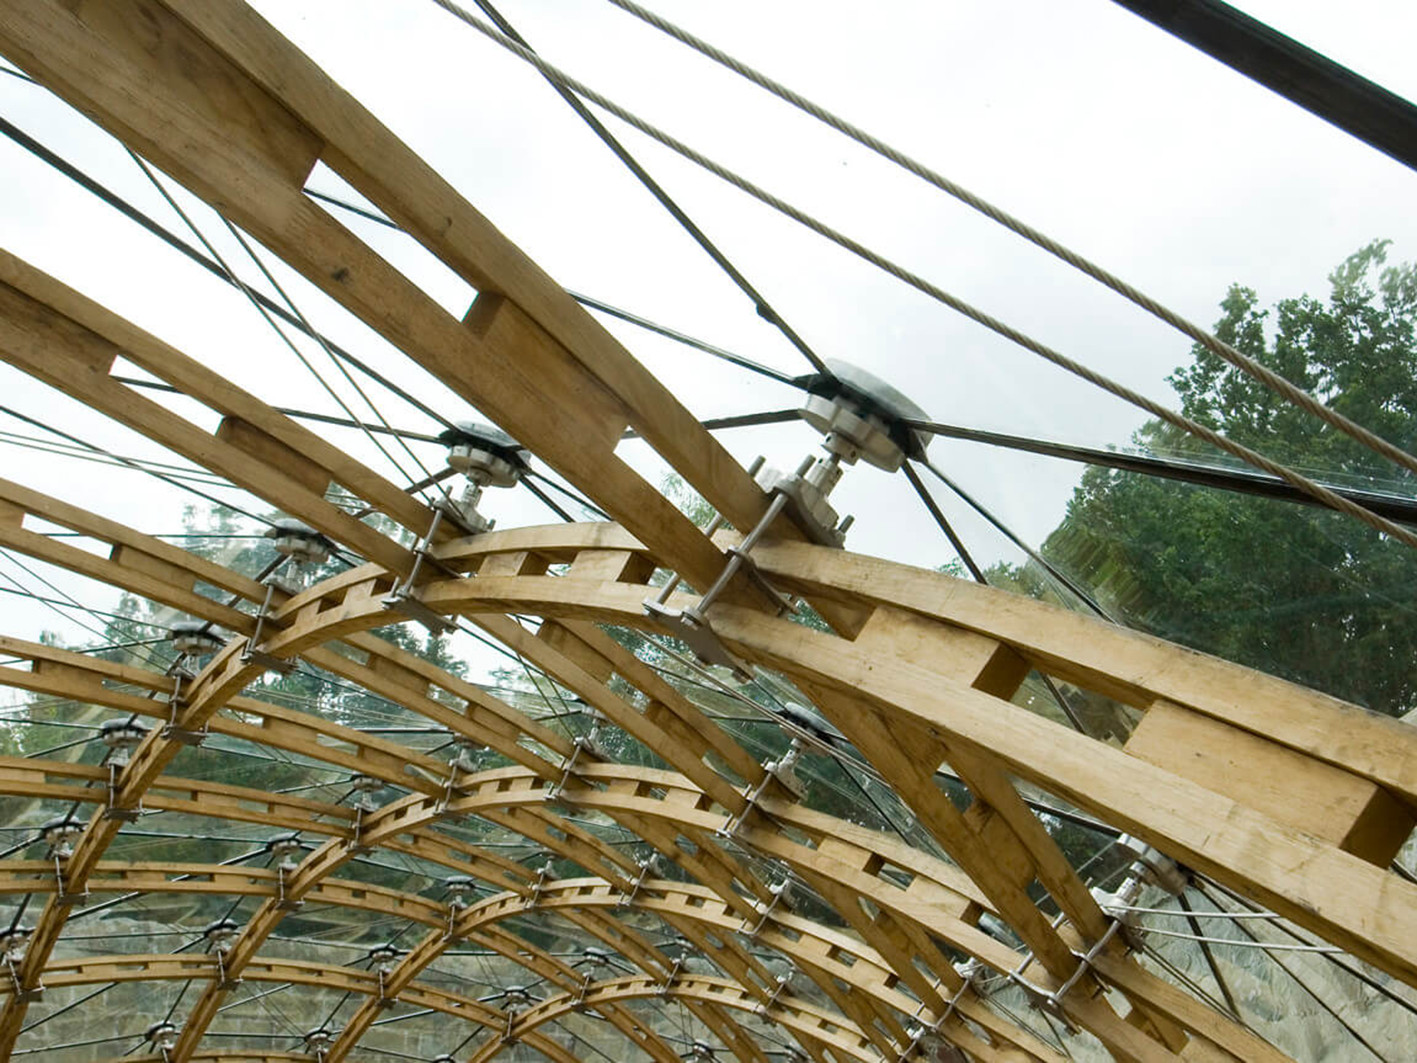
\includegraphics[width=0.48\textwidth]{kent_grid.jpg}\label{fig:kent_a}}
		\hspace*{\fill}
		\subfloat[][Exterior view]{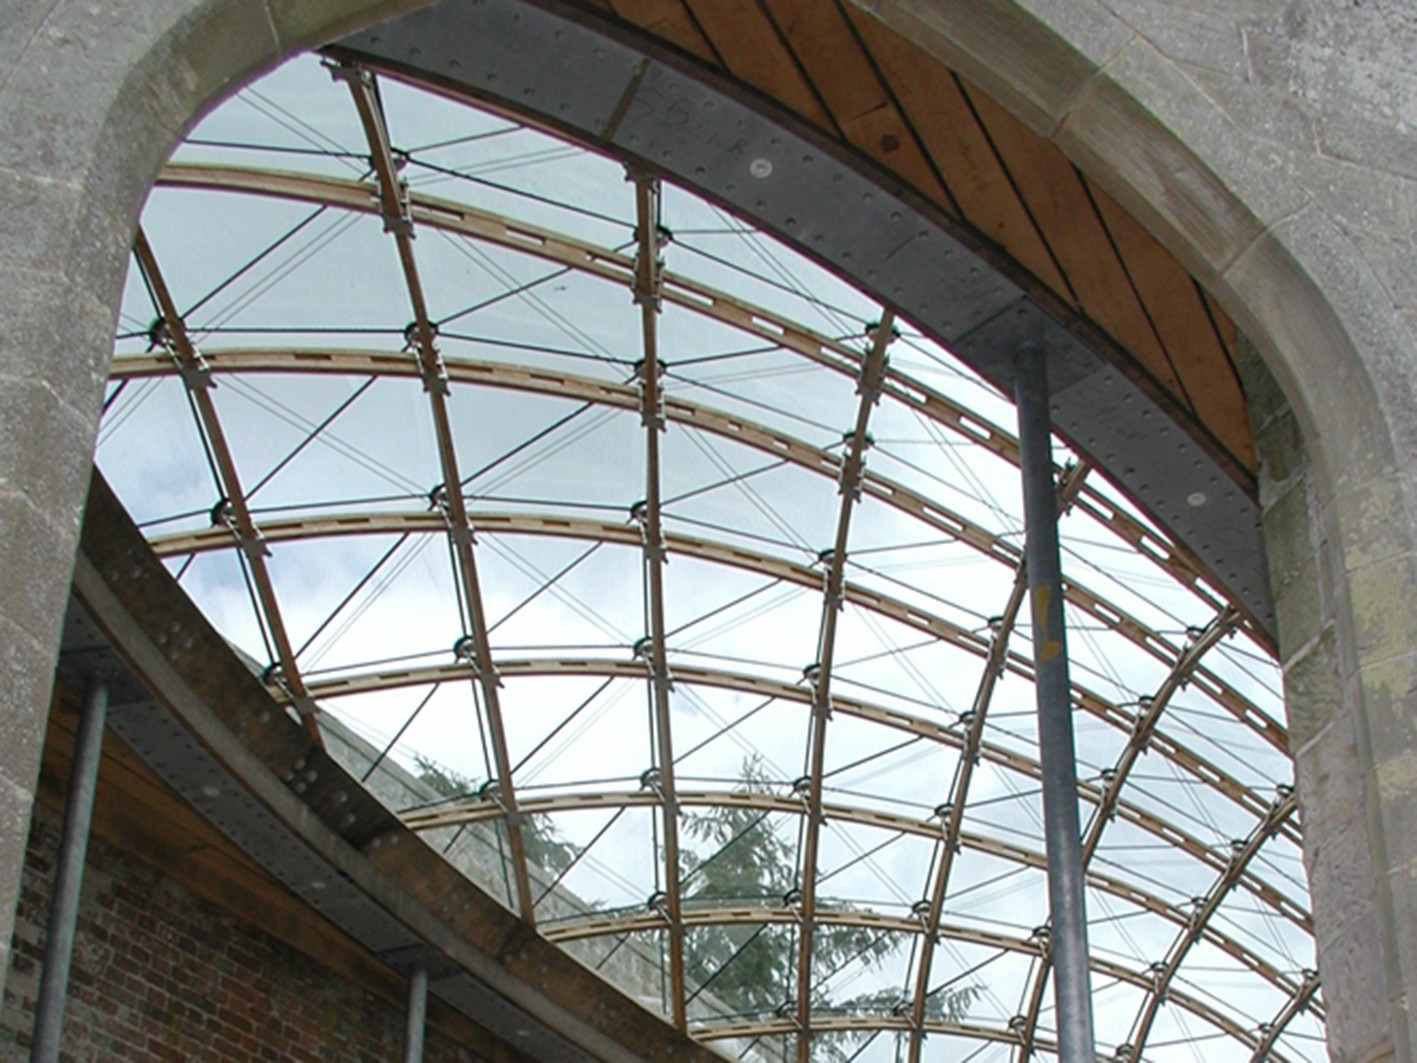
\includegraphics[width=0.48\textwidth]{kent_ext.jpg}\label{fig:kent_b}}
		\vspace{10pt}
		\captionof{figure}[Timber gridshell built in 2007 in Kent, England]{Timber gridshell built in 2007 in Kent, England.}
		\label{fig:kent} 
\end{figure}

However this project embed some interesting innovations. Indeed, this time the gridshell is braced with a bidirectional cable network. Twin cables are employed to facilitate clamping on the node connection, which has been adapted from the previous version developed in Downland. Moreover, this connection is equipped with an additional threaded hole which can received the clamping supports for the glazing (see \cref{fig:kent_a}). The timber shell is then glazed with triangular panels (note that the mesh quadrangles are not planar any more in the deformed configuration).

\subsection{Gridshell in composite materials : a new perpective.}
Based on this groundwork, the Navier laboratory has developed a research program on gridshells for the last decade, focusing on both the use of new materials and the development of more efficient numerical methods \cite{Douthe2007}. These developments have been validated by the construction of two prototypes (Figures \ref{fig:4}a and \ref{fig:4}b) covering were about \SI{150}{m^2}.

In 2011, the laboratory used its expert knowledge for a large-scale project \cite{Baverel2012}, the forum of the Solidays festival (\autoref{fig:4}c). This achievement, built by voluntary workers, has been the first composite material gridshell to house public.

In 2012, the context is favorable for a new achievement named \emph{"Temporary Cathedral of Créteil"}. Although this gridshell has an area very similar to the Solidays one, the project raised new challenges, in particular the challenge of reliability. Indeed, its period of use is at least two years. Additionally, the skills coming from T/E/S/S company made possible important developments such as for doors, lacing edge beam, anchorages and sleeves.

Unlike the two first prototypes, the gridshells built for Solidays and at Créteil are based on a new approach regarding shape-structure relationship. Indeed, thanks to a numerical tool performing the compass method, the geometry of the object is no longer defined as the reversal of a hanging net – in this case, only the flat geometry could be mastered \cite{Addis2013} – but now the flat geometry is straight deducted from the one proposed by the architect.
This new approach opens up new architectural horizons, making possible the exploration of new shapes for gridshells.


\begin{figure}[h]
		\subfloat[][First prototype (2007)]{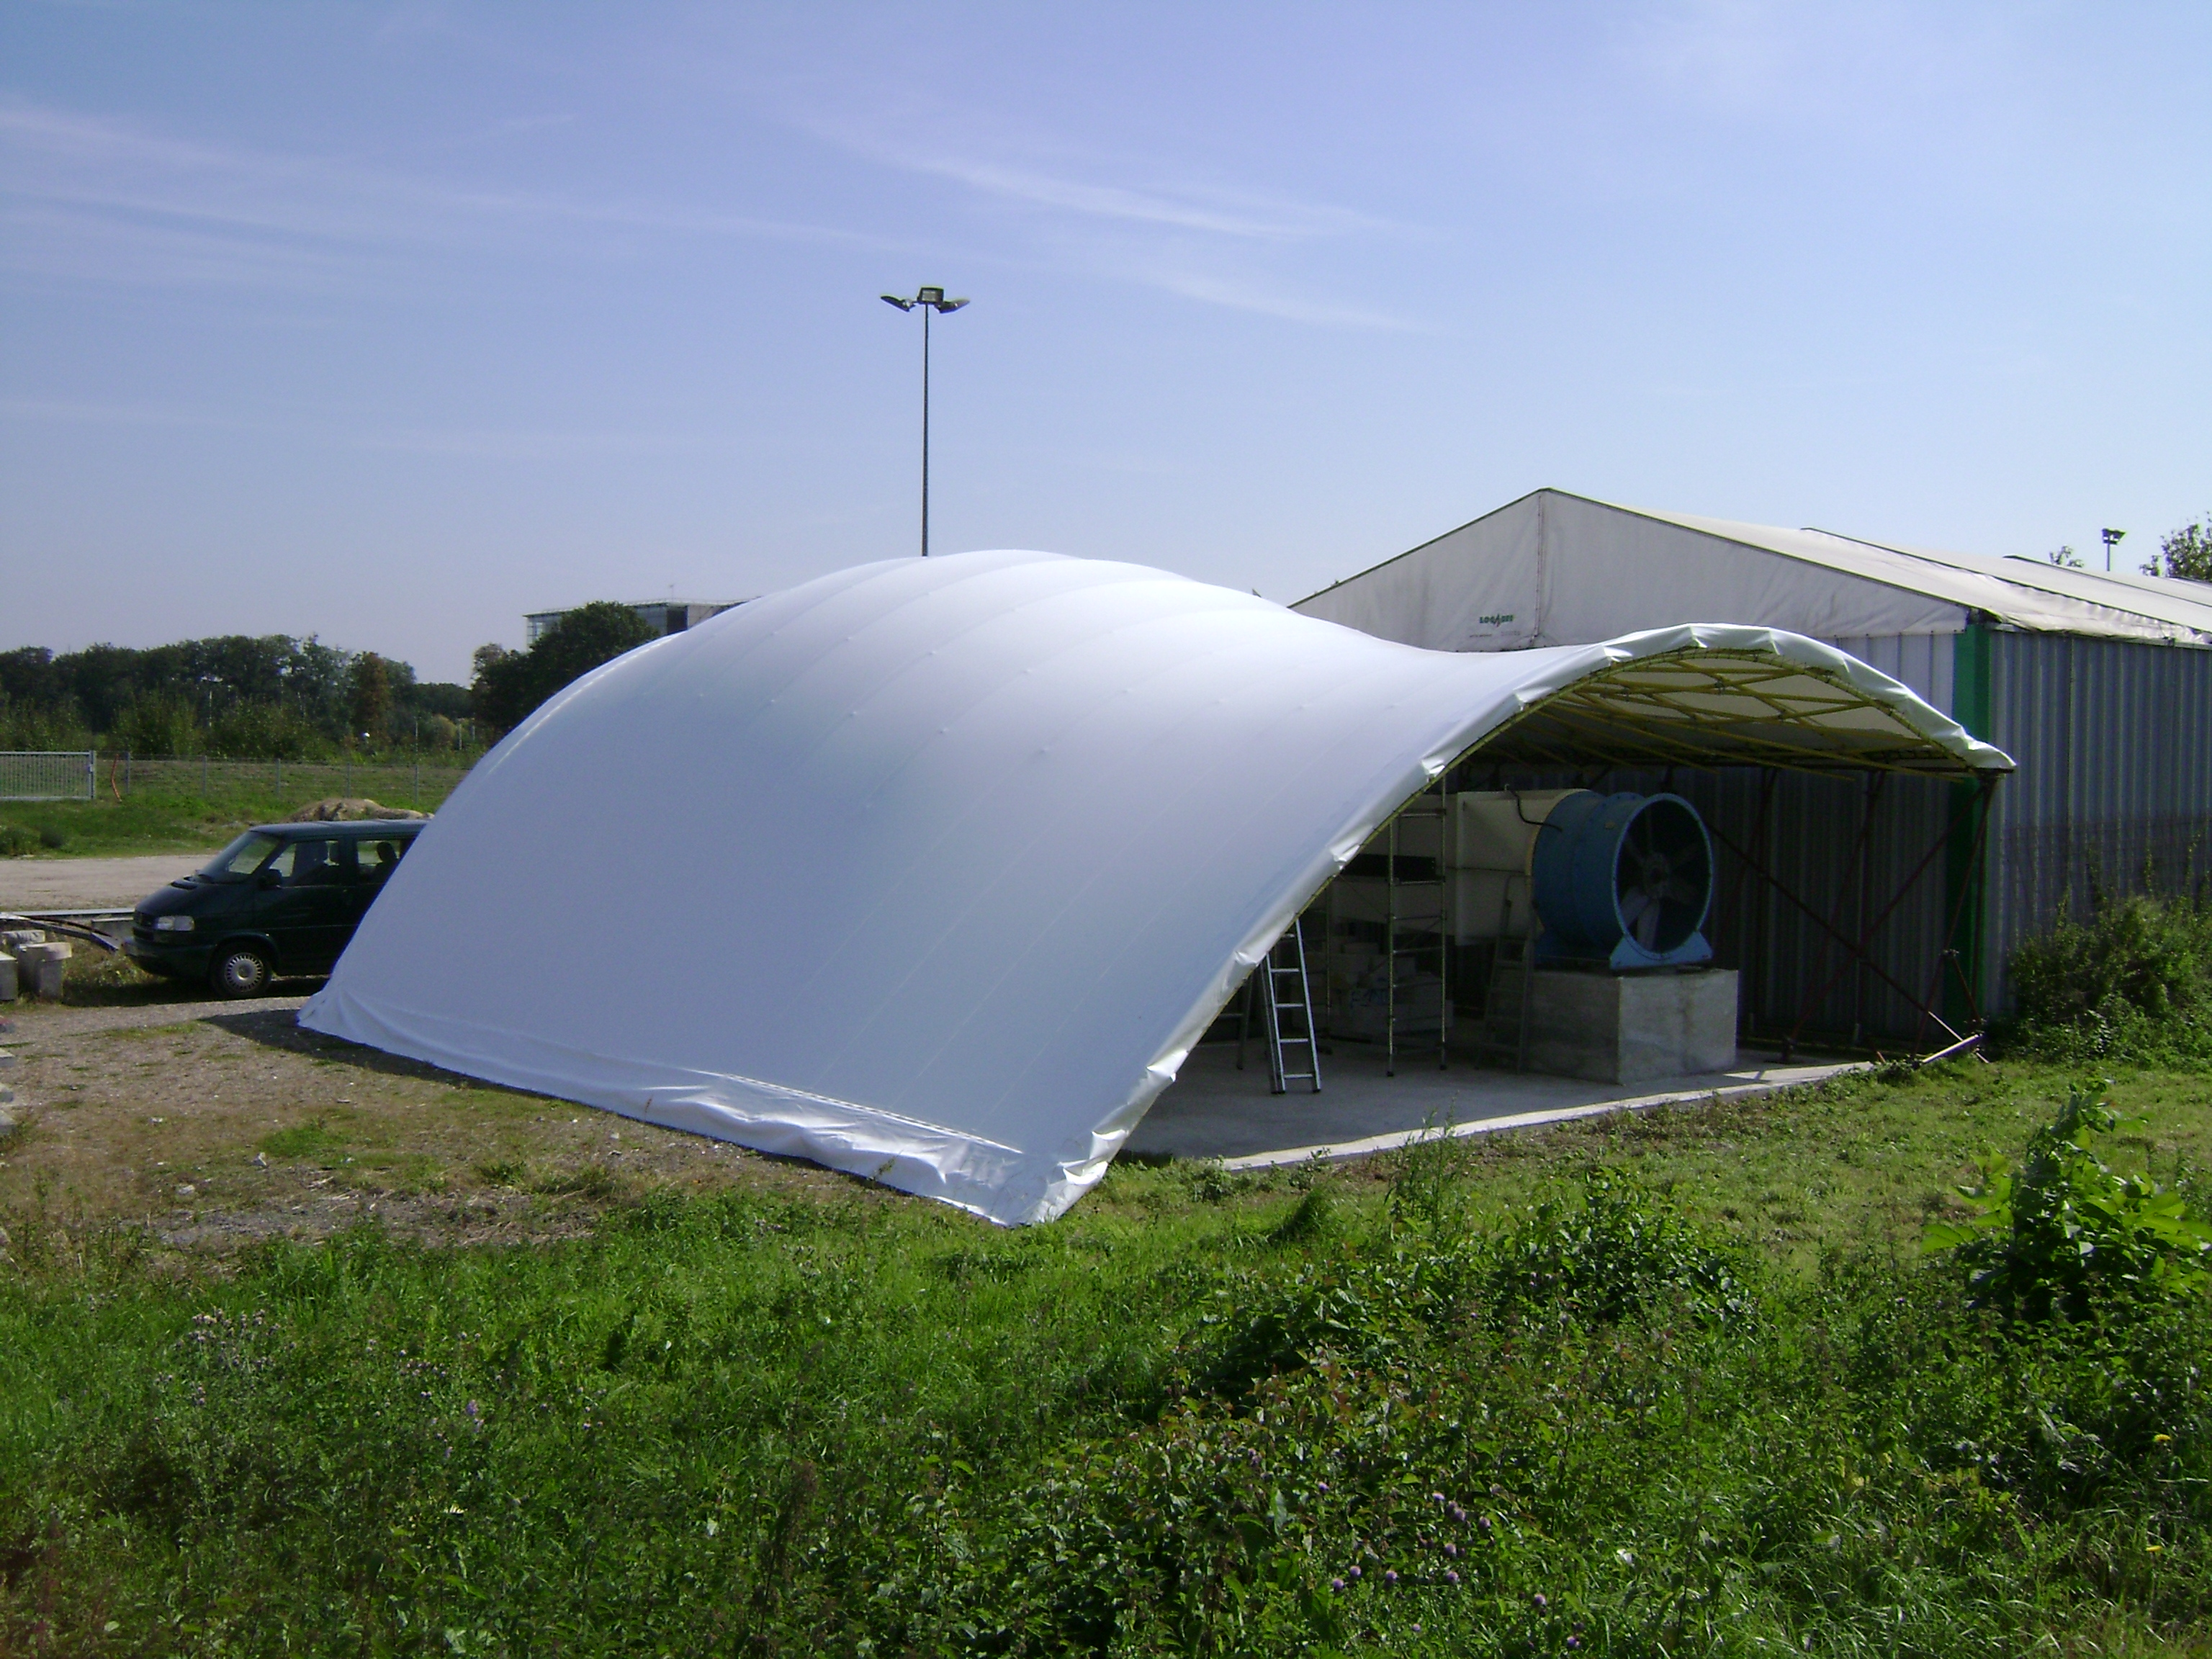
\includegraphics[width=0.48\textwidth]{proto_a.jpg}\label{fig:proto_a}}
		\hspace*{\fill}
		\subfloat[][Second prototype (2008)]{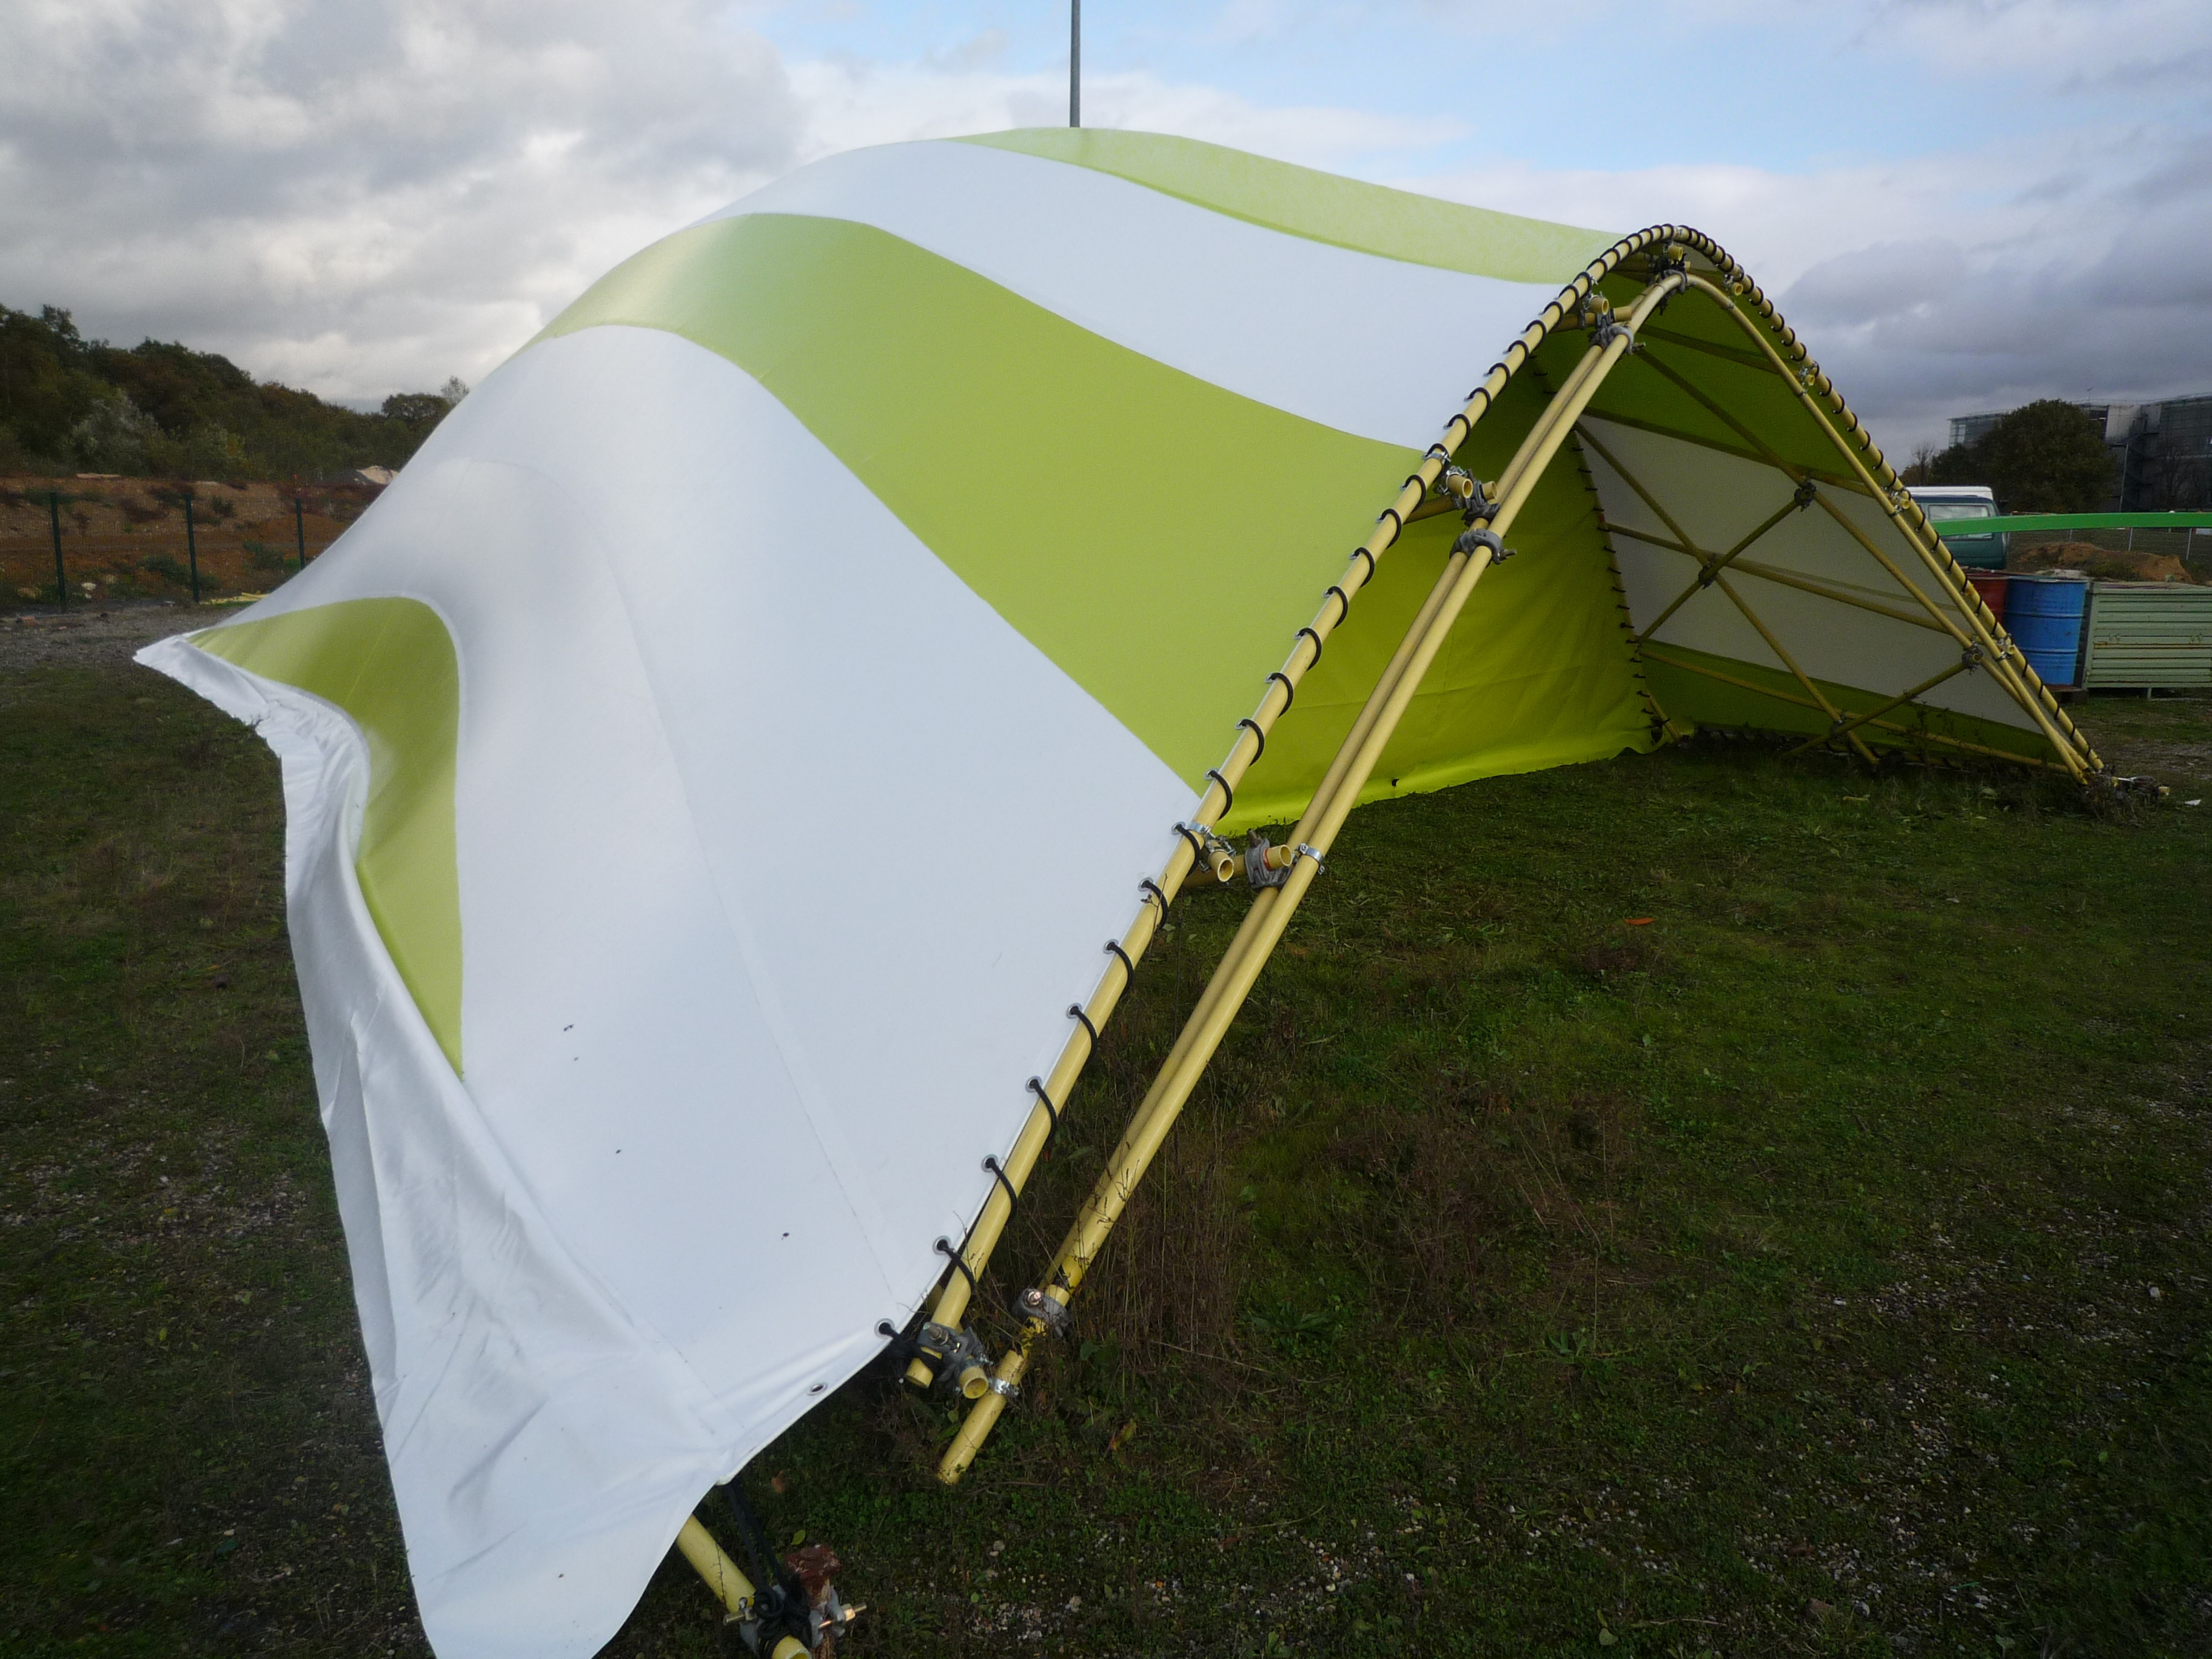
\includegraphics[width=0.48\textwidth]{proto_b.jpg}\label{fig:proto_b}}
		%
		\vspace{10pt}
		\captionof{figure}[GFRP gridshells built in 2007 and 2008 in Noisy-Champs, France]{GFRP gridshells built in 2007 in Noisy-Champs, France.}
		\label{fig:proto}    
\end{figure}

\begin{figure}[h]
		\subfloat[][First prototype (2007)]{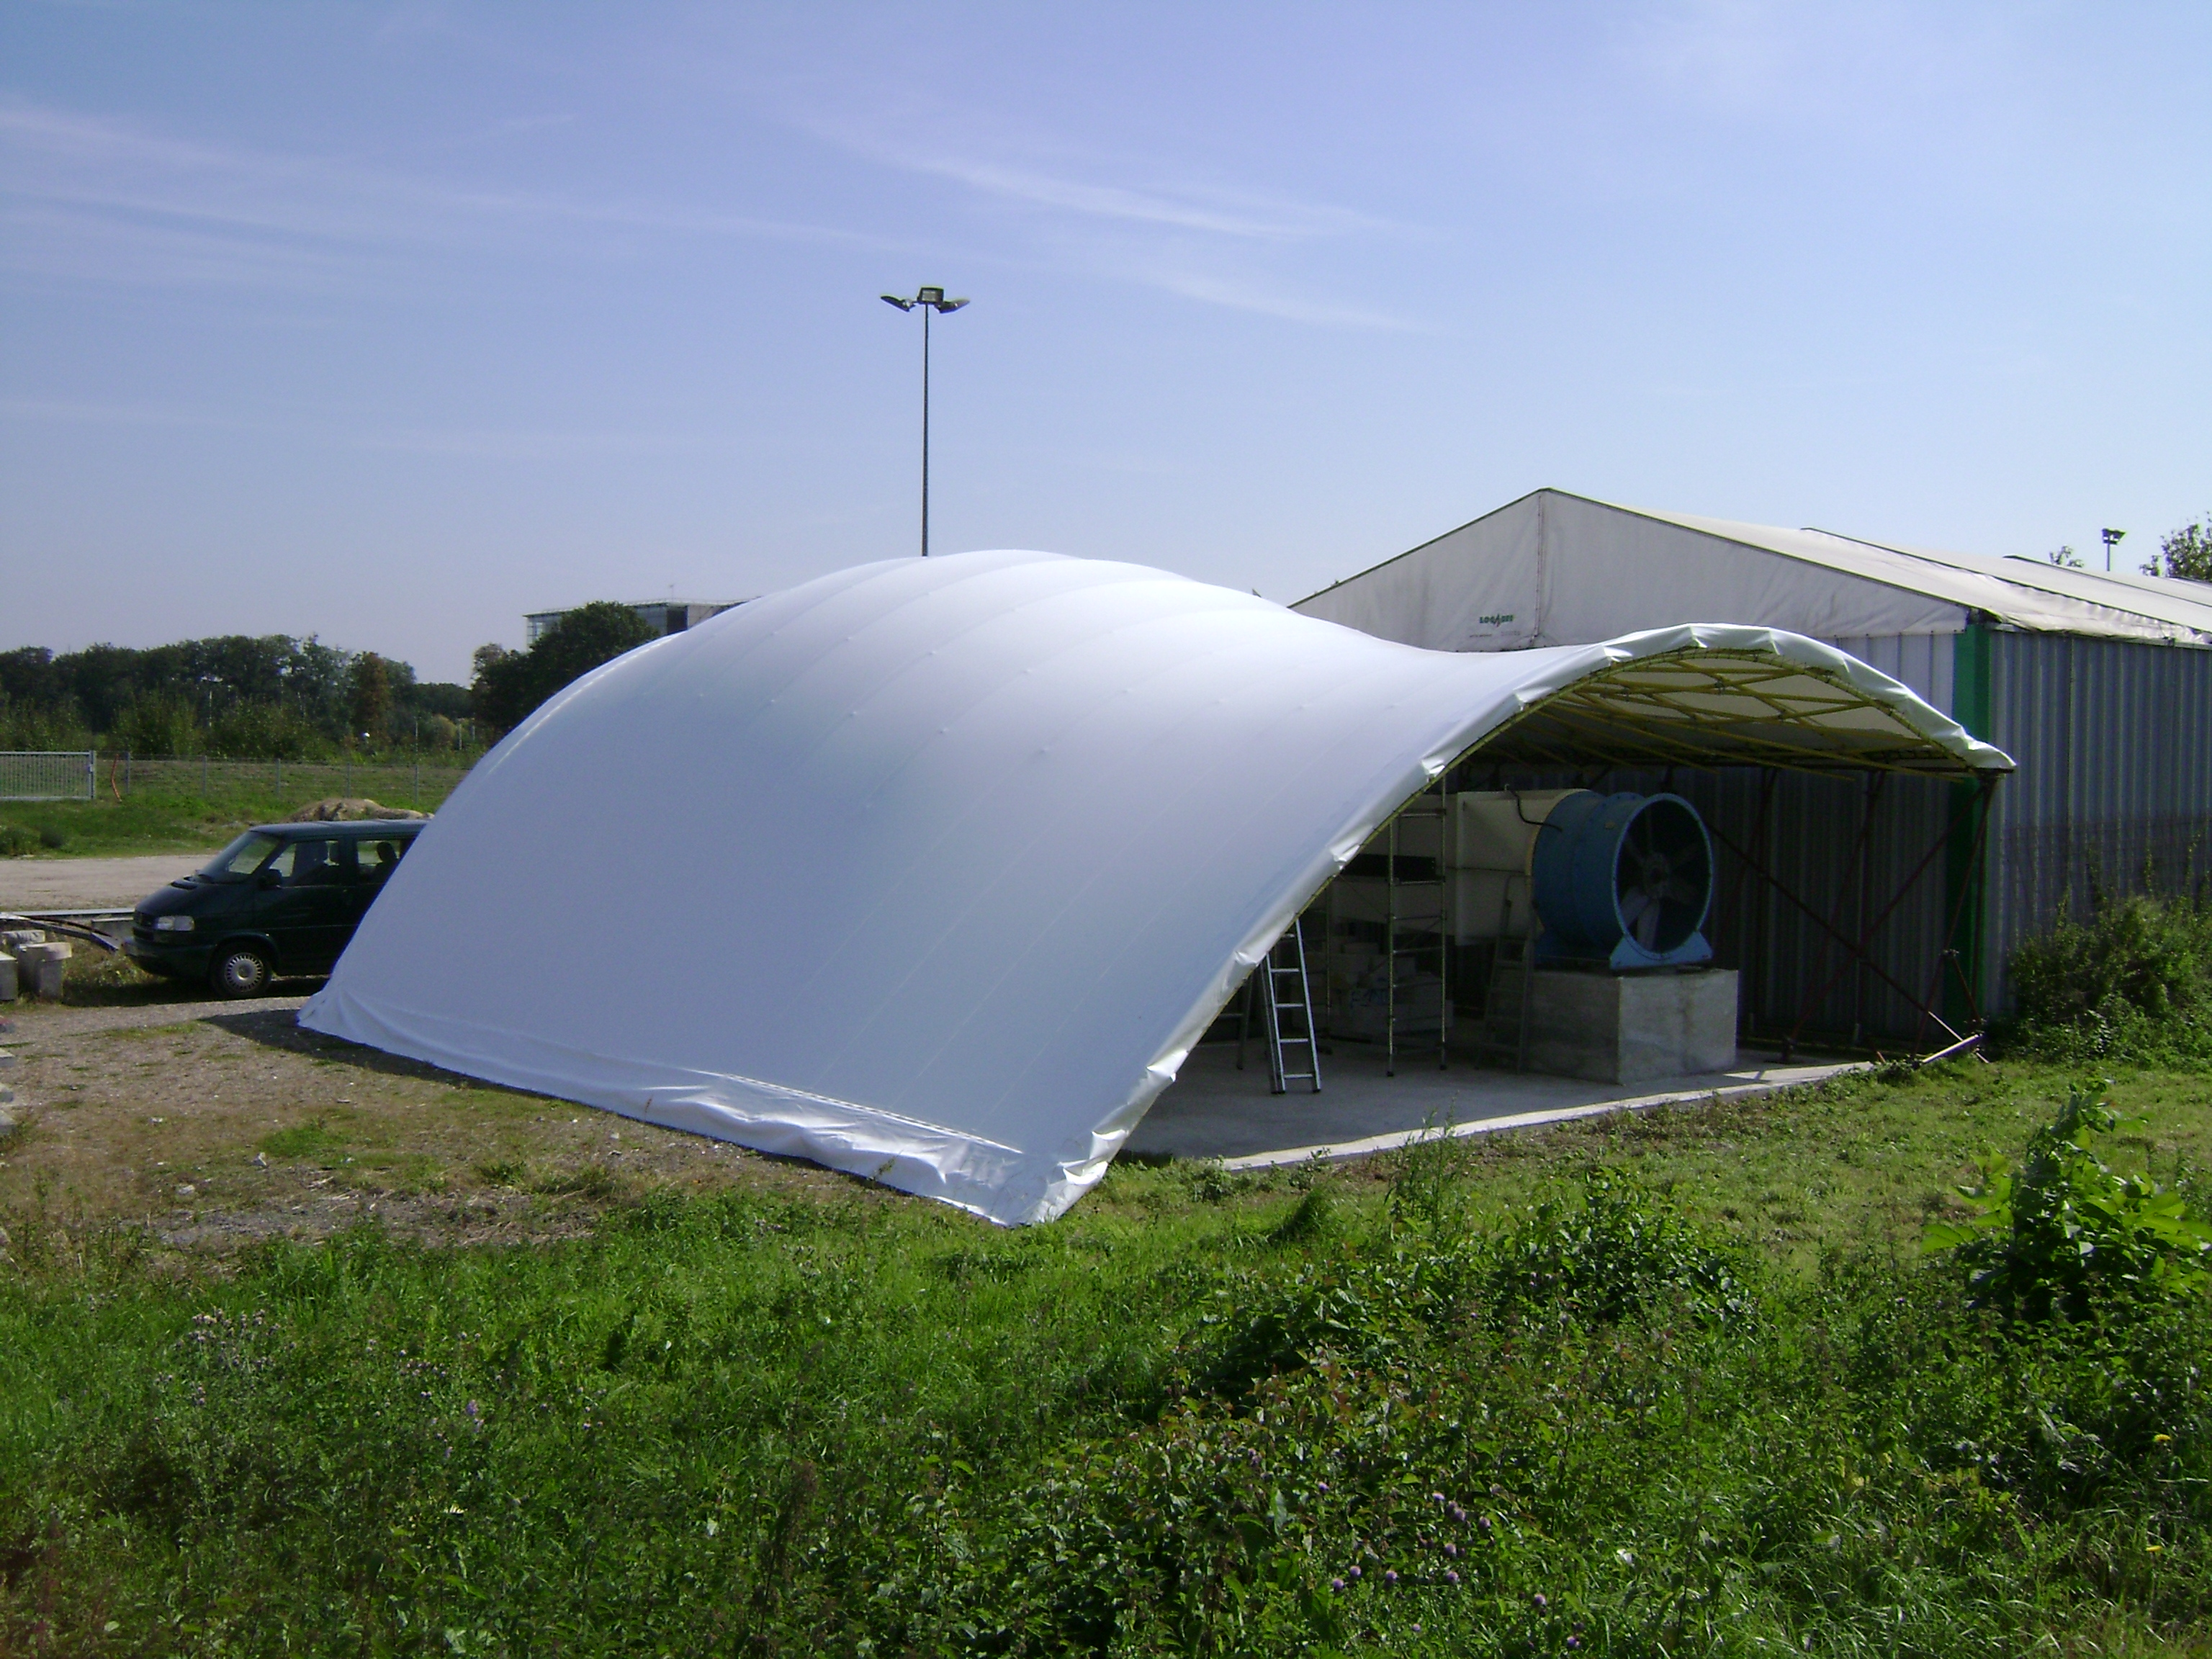
\includegraphics[width=0.48\textwidth]{proto_a.jpg}\label{fig:proto_a}}
		\hspace*{\fill}
		\subfloat[][Second prototype (2008)]{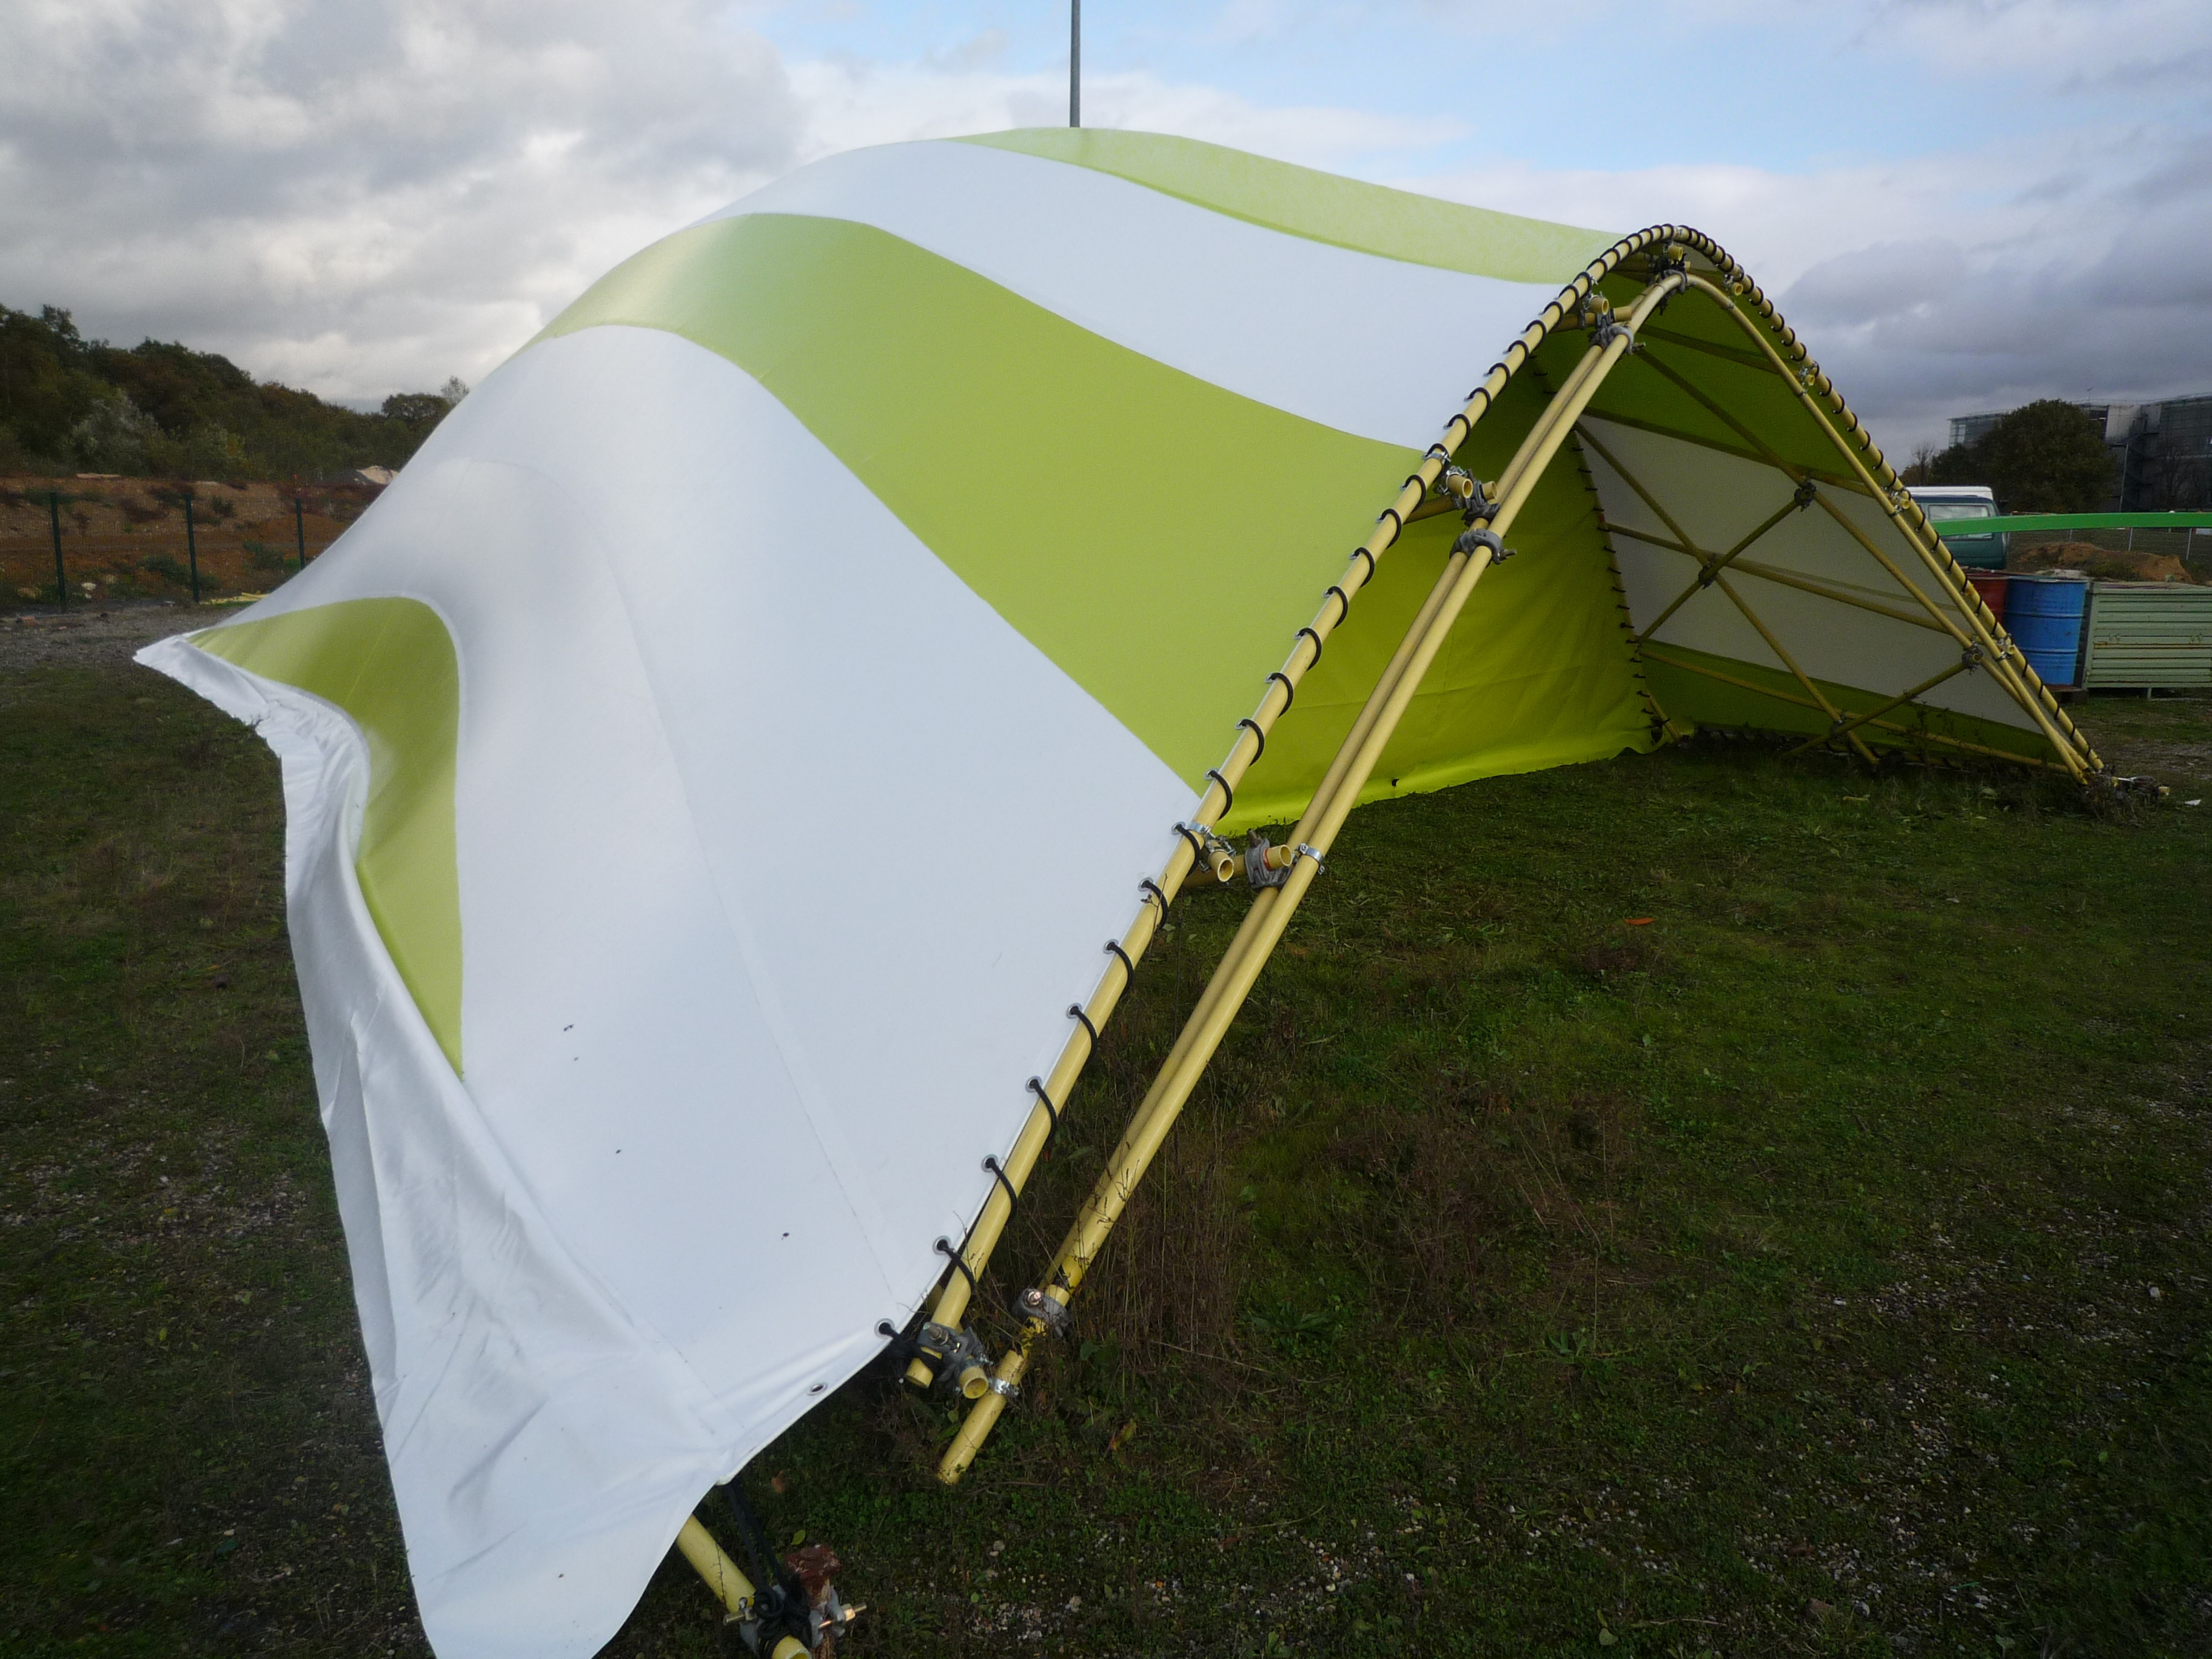
\includegraphics[width=0.48\textwidth]{proto_b.jpg}\label{fig:proto_b}}
		%
		\vspace{10pt}
		\captionof{figure}[GFRP gridshells built in 2007 and 2008 in Noisy-Champs, France]{GFRP gridshells built in 2007 in Noisy-Champs, France.}
		\label{fig:proto}    
\end{figure}


Toledo 1 : \cite{DAmico2014}
Toledo 2 : \cite{DAmico2015a}


\clearpage
\section{Research works in the field of elastic gridshells : a review}

\cite{Labonnote2016}

\subsection{Formfinding and structural analysis}
Les méthodes numériques de Day, Barnes, Adriaenssen, Douthe, Lefevre, Tayeb
3/6/4 DOF, prise en compte de la torsion.
\citet{Adriaenssens1999, Adriaenssens2001}
\cite{Barnes2013}
\cite{DAmico2014}
\cite{DAmico2016}

\cite{DuPeloux2015}
\citet{Malek2012}

\subsection{Stability}
Flambement (Malek, Mesnil, Lefevre)
\citet{Mesnil2013}
\citet{Mesnil2015a}
\citet{Mesnil2017a}
\citet{Lefevre2015}
\citet{Tayeb2013}

\subsection{Gridfinding}
Le formfinding vs. grid finding (COmpas Lionel, Compas Baptise, GFFT, Compas Yannick singularité, Lina)
Elisa Fuentes

\cite{Pone2016}
\cite{DuPeloux2011}
\cite{Lafuente2015}
\cite{Masson2017}

\subsection{Morphology}
\cite{Douthe2016a}
Mesnil
Description analytique de la forme (C. Williams)

\subsection{New materials}
Les matériaux composites

\subsection{Erection}
Les méthodes de montage. L'inflatable(Otto, Pugnale, Quinn)
\cite{IL10}
\cite{Quinn2014}
\cite{Liuti2015}
\citet{Liuti2016}

\subsection{Cladding}
Une reflexion sur l'enveloppe (booby ENPC).
\citet{Lafuente2014}
\citet{Cuvilliers2017}
\cite{Filz2015}

\subsection{Rationalization}
La simplification (gridshell.it => ZA, UTSA, Cluj, quaternion + Navier, Navier)

\subsection{Robotisation}
La robotisation de la production (ENPC)
ZA

\subsection{Structural optimisation}
Optimisation des sections
\cite{DAmico2015}










\clearpage

\subsubsection{Des pistes ouvertes}











\begin{landscape}%
\begin{table}[p]
\centering\small
\ra{1.3}
%\begin{fullpage}
 	\begin{tabularx}{20cm}{@{}l X l l l l l l r@{}}
	\toprule
%		&				&		&				&			&			& \multicolumn{2}{c}{Project Team}						& 	\\ \cmidrule(l){7-8}
 	N	& Nickname		& Year	& City			& Country		& Type		& Architecte 			& Enginneer			& Ref \\ 
	\midrule
	1 	& Berkeley		& 1962	& Berkeley		& USA		& Prototype	& F. Otto	 			& F. Otto				& \cite{IL10} \\
	2 	& Essen			& 1962	& Essen			& Germany	& Pavilion		& F. Otto	 			& F. Otto				& \cite{IL10} \\
	3 	& German Pavillion	& 1967	& Montreal		& Canada		& Pavilion		& F. Otto	 			& F. Otto				& \cite{IL10} \\
	4 	& Seibu			& 1973	& hannover			& Japan		& Prototype	& K. Matsushita	 		& T. Shirayanagi		& \cite[p.~245]{IL13} \\
	5 	& Ahmedabad		& 1976	& Ahmedabad		& India		& Building		& G. Sarabhai 			& G. Ramaswamy		& \cite[p.~249]{IL13} \\
	6 	& Bamboo			& 1976	& London			& England		& Workshop	& J. Park 				& B. Oleiko			& \cite{IL13} \\

	7 	& Mexico			& 1973	& hannover			& Japan		& Protorype	& J. Hennicke			& J. Hennicke			& \cite{IL13} \\
	8 	& Mexico			& 1973	& hannover			& Japan		& Workshop	& J. Hennicke			& J. Hennicke			& \cite{IL13} \\

	9 	& Mexico			& 1977	& Zitacuaro		& Mexico		& House		& F. Montero			& F. Montero			& \cite{IL13} \\

	\midrule
	10 	& Mannheim		& 1975	& Mannheim		& Germany	& Building		& C. Mutschler 	 		& Arup + F. Otto  		& \cite{IL13} \\
	11 	& Japan Pavilion	& 2000	& Hannover		& Germany	& Pavilion		& S. Ban + F. Otto		& Buro Happold 		& \cite{} \\
	12 	& Downland		& 2002	& Singleton		& England		& Building		& E. Cullinan	 		& Buro Happold		& \cite{Harris2003} \\
	13 	& Savill			& 2006	& Englefield		& England		& Building		& G. Howells			& Buro Happold		& \cite{Harris2008} \\
	14 	& Chiddingstone	& 2007	& Chiddingstone	& England		& Canopy		& P. Hulbert			& Buro Happold		& \cite{} \\
	
	\bottomrule
 	\end{tabularx}
\captionof{table}[Key numbers]{Key numbers.}
%\end{fullpage}
\end{table}
\end{landscape}%



\begin{landscape}%
\begin{table}[p]
\centering\small
\ra{1.3}
%\begin{fullpage}
 	\begin{tabular}{@{}llll  lllllr@{}}
	\toprule
%    &         & 	          & Type & City & Country & Architecte & Engineer & Page & Citation \\
N & Year & Nickname & Type & City & Country & Architecte & Engineer & Page & Citation\\
1 & 1962 & Experimental structure  & Workshop & Berkeley & USA & Students & F. Otto & p.~270 & \cite{IL10}\\
2 & 1962 & Exhibition pavilion & Pavilion & Essen & Germany & F. Otto & F. Otto & p.~272 & \cite{IL10}\\
3 & 1967 & German Pavilion & Pavilion & Montreal & Canada & F. Otto & Lehonardt & p.~274 & \cite{IL10}\\
4 & 1973 & Seibu & Experiment & hannover & Japan & IL & IL & p.~245 & \cite{IL13}\\
5 & 1974 & Basket shell & Experiment & Amehabad & India & G. Sarabhai & IL & p.~304 & \cite{IL10}\\
6 & 1974 & Experimental structure  & Experiment & London & England & Students & Arup + IL & p.~306 & \cite{IL10}\\
7 & 1975 & Mannheim Multihalle & Building & Mannheim & Germany & C. Mutshler & Arup + IL & p.~308 & \cite{IL10}\\
8 & 1973 & Ferrocement gridshell & Building & Ahmedabad & India & G. Sarabhai & G. Ramaswamy + IL & p.~248 & \cite{IL13}\\
9 & 1976 & AA Bamboo Latice Shell & Workshop & London & England & Students & J. Park + B. Oleiko & p.~255 & \cite{IL13}\\
10 & 1976 & Test structure of a gridshell & Experiment & Stuttgart & Germany & Students & J. Hennicke & p.~298 & \cite{IL10}\\
11 & 1977 & Small Pavilion & Workshop & Mexico City & Mexico & Students & J. Hennicke & p.~258 & \cite{IL13}\\
11 & 1977 & Small Greenhouse & Workshop & Zitacuaro & Mexico & Students & F. Montero & p.~260 & \cite{IL13}\\
12 & 1977 & Experimental structure & Workshop & Mexico City & Mexico & Students & F. Montero & p.~270 & \cite{IL13}\\
13 & 1977 & Experimental structure & Workshop & Mexico City & Mexico & Students & F. Montero & p.~270 & \cite{IL13}\\
14 & 1995 & Westminster Lodge & Building & Dorset & England & E. Cullinan & F. Otto + Happold & p.~90 & \cite{Burton1998}\\
15 & 1998 & Earth Center & Building & Doncaster & England & Grant & Happold &  & \\
16 & 2000 & Japan Pavilion & Pavilion & Hannover & Germany & S. Ban + F. Otto & Happold &  & \cite{Ban2006}\\
17 & 2002 & Downland & Building & Downland & England & E. Cullinan & Happold + C. William &  & \cite{Harris2003}\\
18 & 2003 & Life Science Centre Trust & Building & Pishwanton & England &  &  &  & \\
19 & 2006 & Savill & Building & Savill & England & G. Howells & Happold + C. William &  & \cite{Harris2008}\\
20 & 2007 & Chiddingstone Orangery & Roofing & Kent & England & P. Hulbert & Happold &  & \\
21 & 2007 & ENPC & Experiment & Noisy-Champs & France & Navier & Navier &  & \cite{Douthe2006}\\
22 & 2011 & Solidays & Pavilion & Paris & France & ENPC & Navier + T/E/S/S &  & \cite{Baverel2012}\\
23 & 2012 & Toledo & Workshop & Naples & Italy & gridshell.it & B. D'Amico &  & \cite{DAmico2014}\\
24 & 2013 & Créteil & Building & Créteil & France & T/E/S/S & T/E/S/S + Navier &  & \cite{DuPeloux2016}\\
25 & 2014 & Toledo 2.0 & Workshop & Naples & Italy & gridshell.it & B. D'Amico &  & \cite{DAmico2015a}\\
26 & 2016 & JPO & Pavilion & Toulouse & France & Quaternion & Navier + Terrell &  & \\
27 & 2016 & FAV & Pavilion & Montpellier & France & Quaternion & Navier + Terrell &  & \\
28 & 2016 & CLC & Workshop & Noisy-Champs & France & ENPC & Navier &  & \\
27 & 2016 & Trondheim & Workshop & Trondheim & Norway & Students & NTNU &  & \cite{Mork2016}\\
 	\end{tabular}
\captionof{table}[Key numbers]{Key numbers.}
%\end{fullpage}
\end{table}
\end{landscape}%


\clearpage

\begin{landscape}%
\begin{table}[p]
\centering
\ra{1.1}
%\begin{fullpage}
 	\begin{tabularx}{20cm}{@{}lll rrrXXX@{}}
	\toprule
		&			& \multicolumn{2}{c}{Project} 			& \multicolumn{3}{c}{Structure}	 	\\
	\cmidrule(l){3-4} \cmidrule(l){5-7}
 	Year & Nickname 	& Country		& Duration			& Material 	& Layer	& Pitch		\\ 
	\midrule
	1975	& Mannheim	& Germany	& LT					& hemlock	 	& double	& \SI{0.5}{m}	\\	
	\bottomrule
 	\end{tabularx}
\captionof{table}[Key numbers]{Key numbers.}
%\end{fullpage}
\end{table}
\end{landscape}%




\clearpage

\footnote{German pavilion 1967 : \url{https://www.youtube.com/watch?v=Z0mtFMoseUk}}
\footnote{German pavilion 1967 : \url{http://www.uncubemagazine.com/magazine-33-15508949.html/page1}}





\section{Gridshell structure : definition and classification}
\subsection{Historic overview}
\subsection{Rigid gridshell}



\begin{figure}[h]
		\captionsetup[subfloat]{captionskip=10pt}
		\subfloat[][Forum Café, Solidays (2011).]{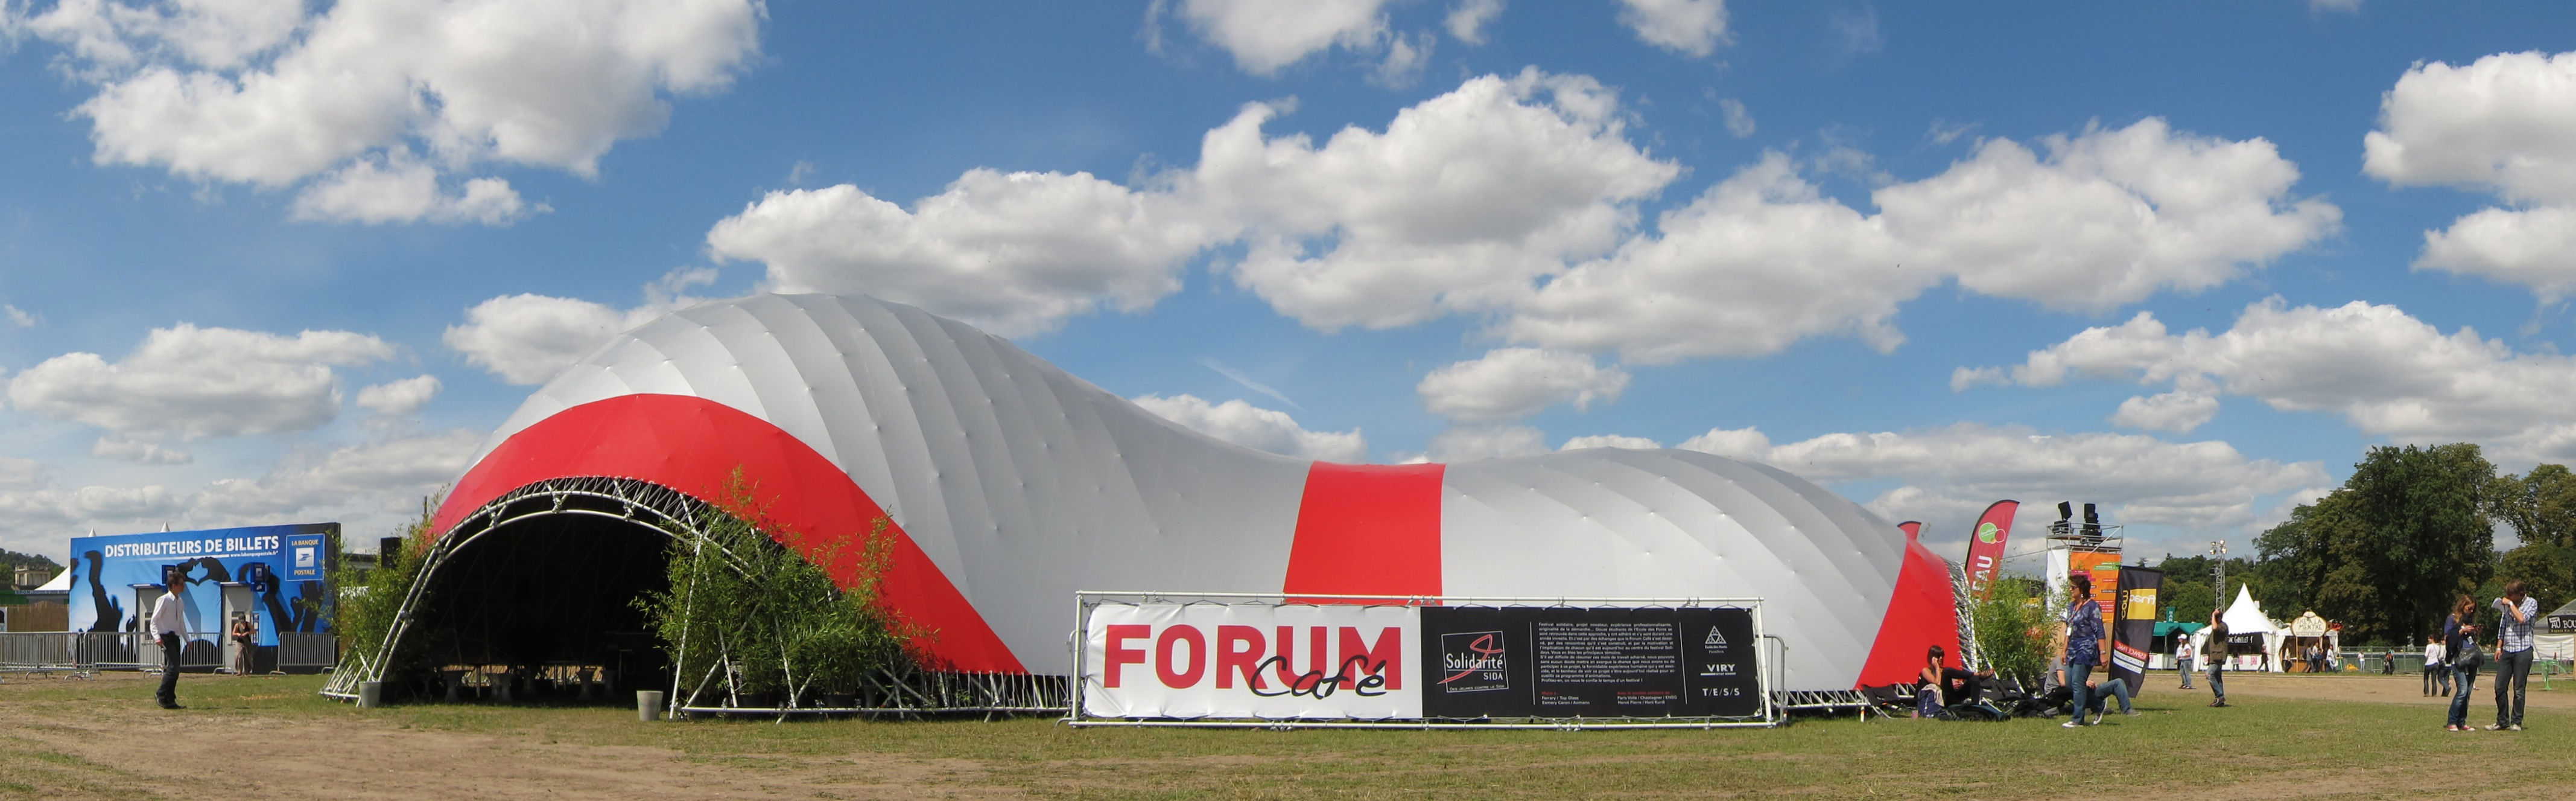
\includegraphics[width=1\textwidth]{solidays.jpg}\label{fig:solidays}}\\
		\subfloat[][Prototype (2007).]{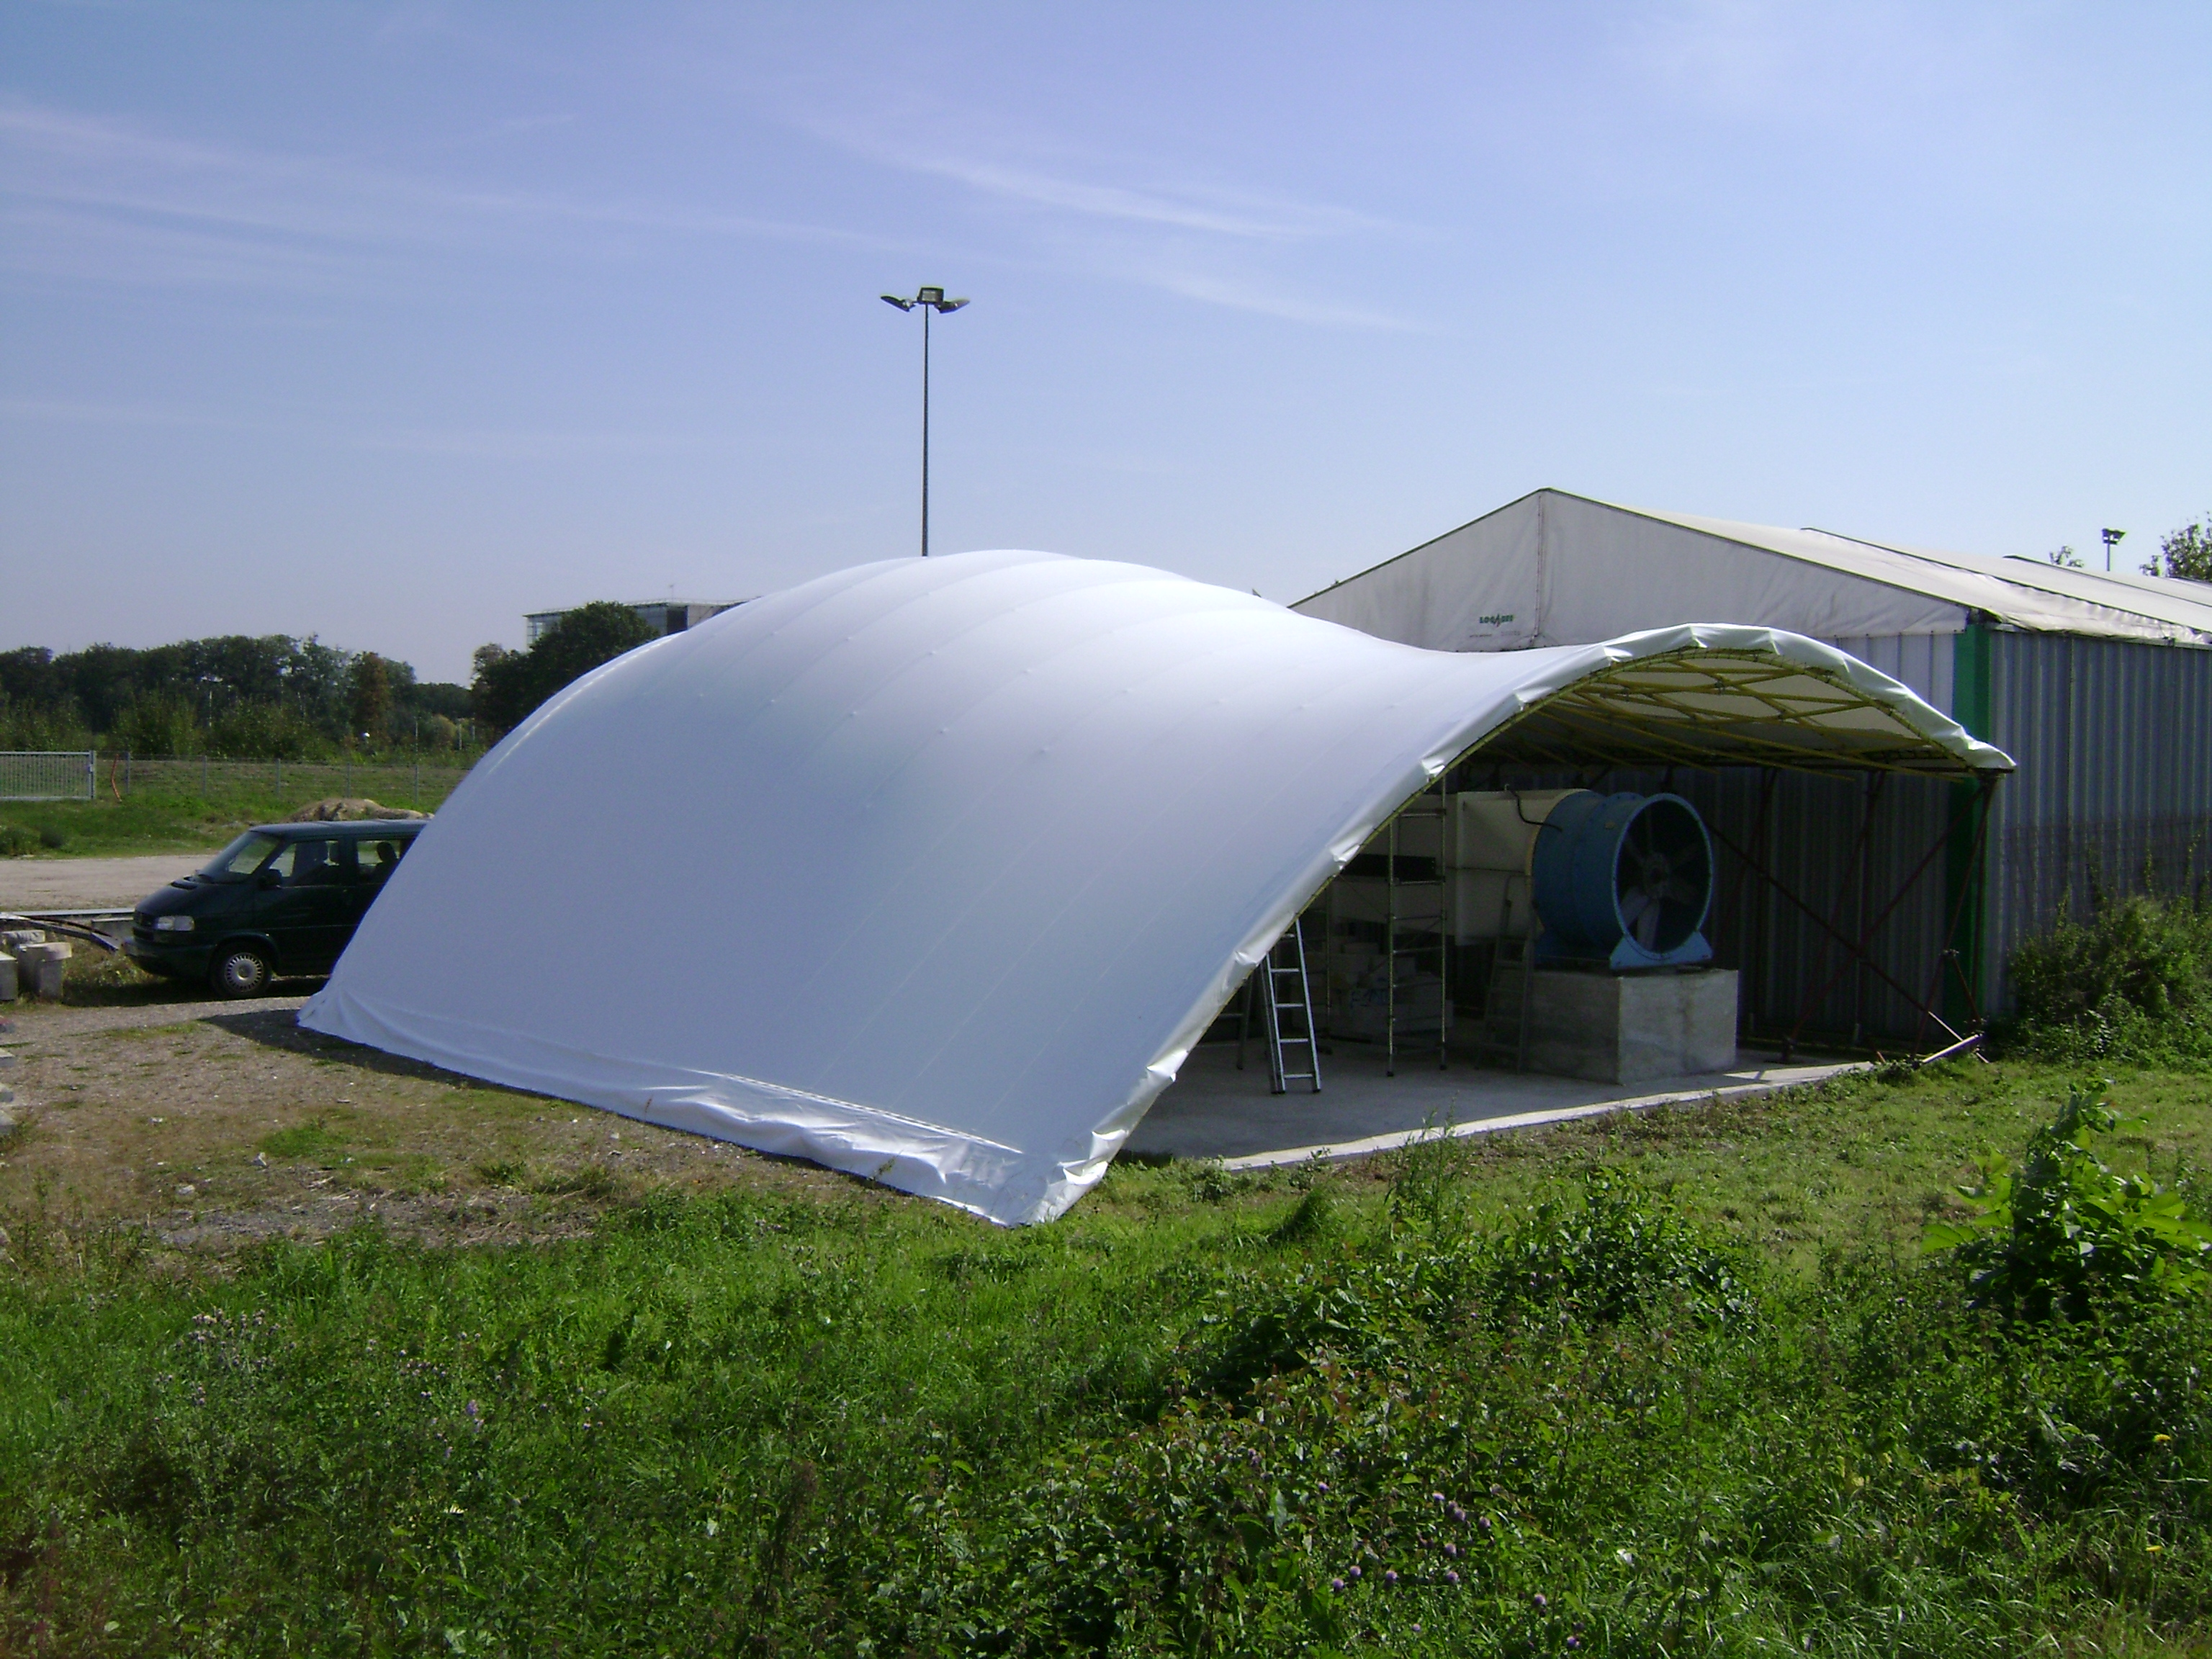
\includegraphics[width=0.48\textwidth]{proto_a.jpg}\label{fig:proto_a}}
		\hspace*{\fill}
		\subfloat[][Prototype (2008).]{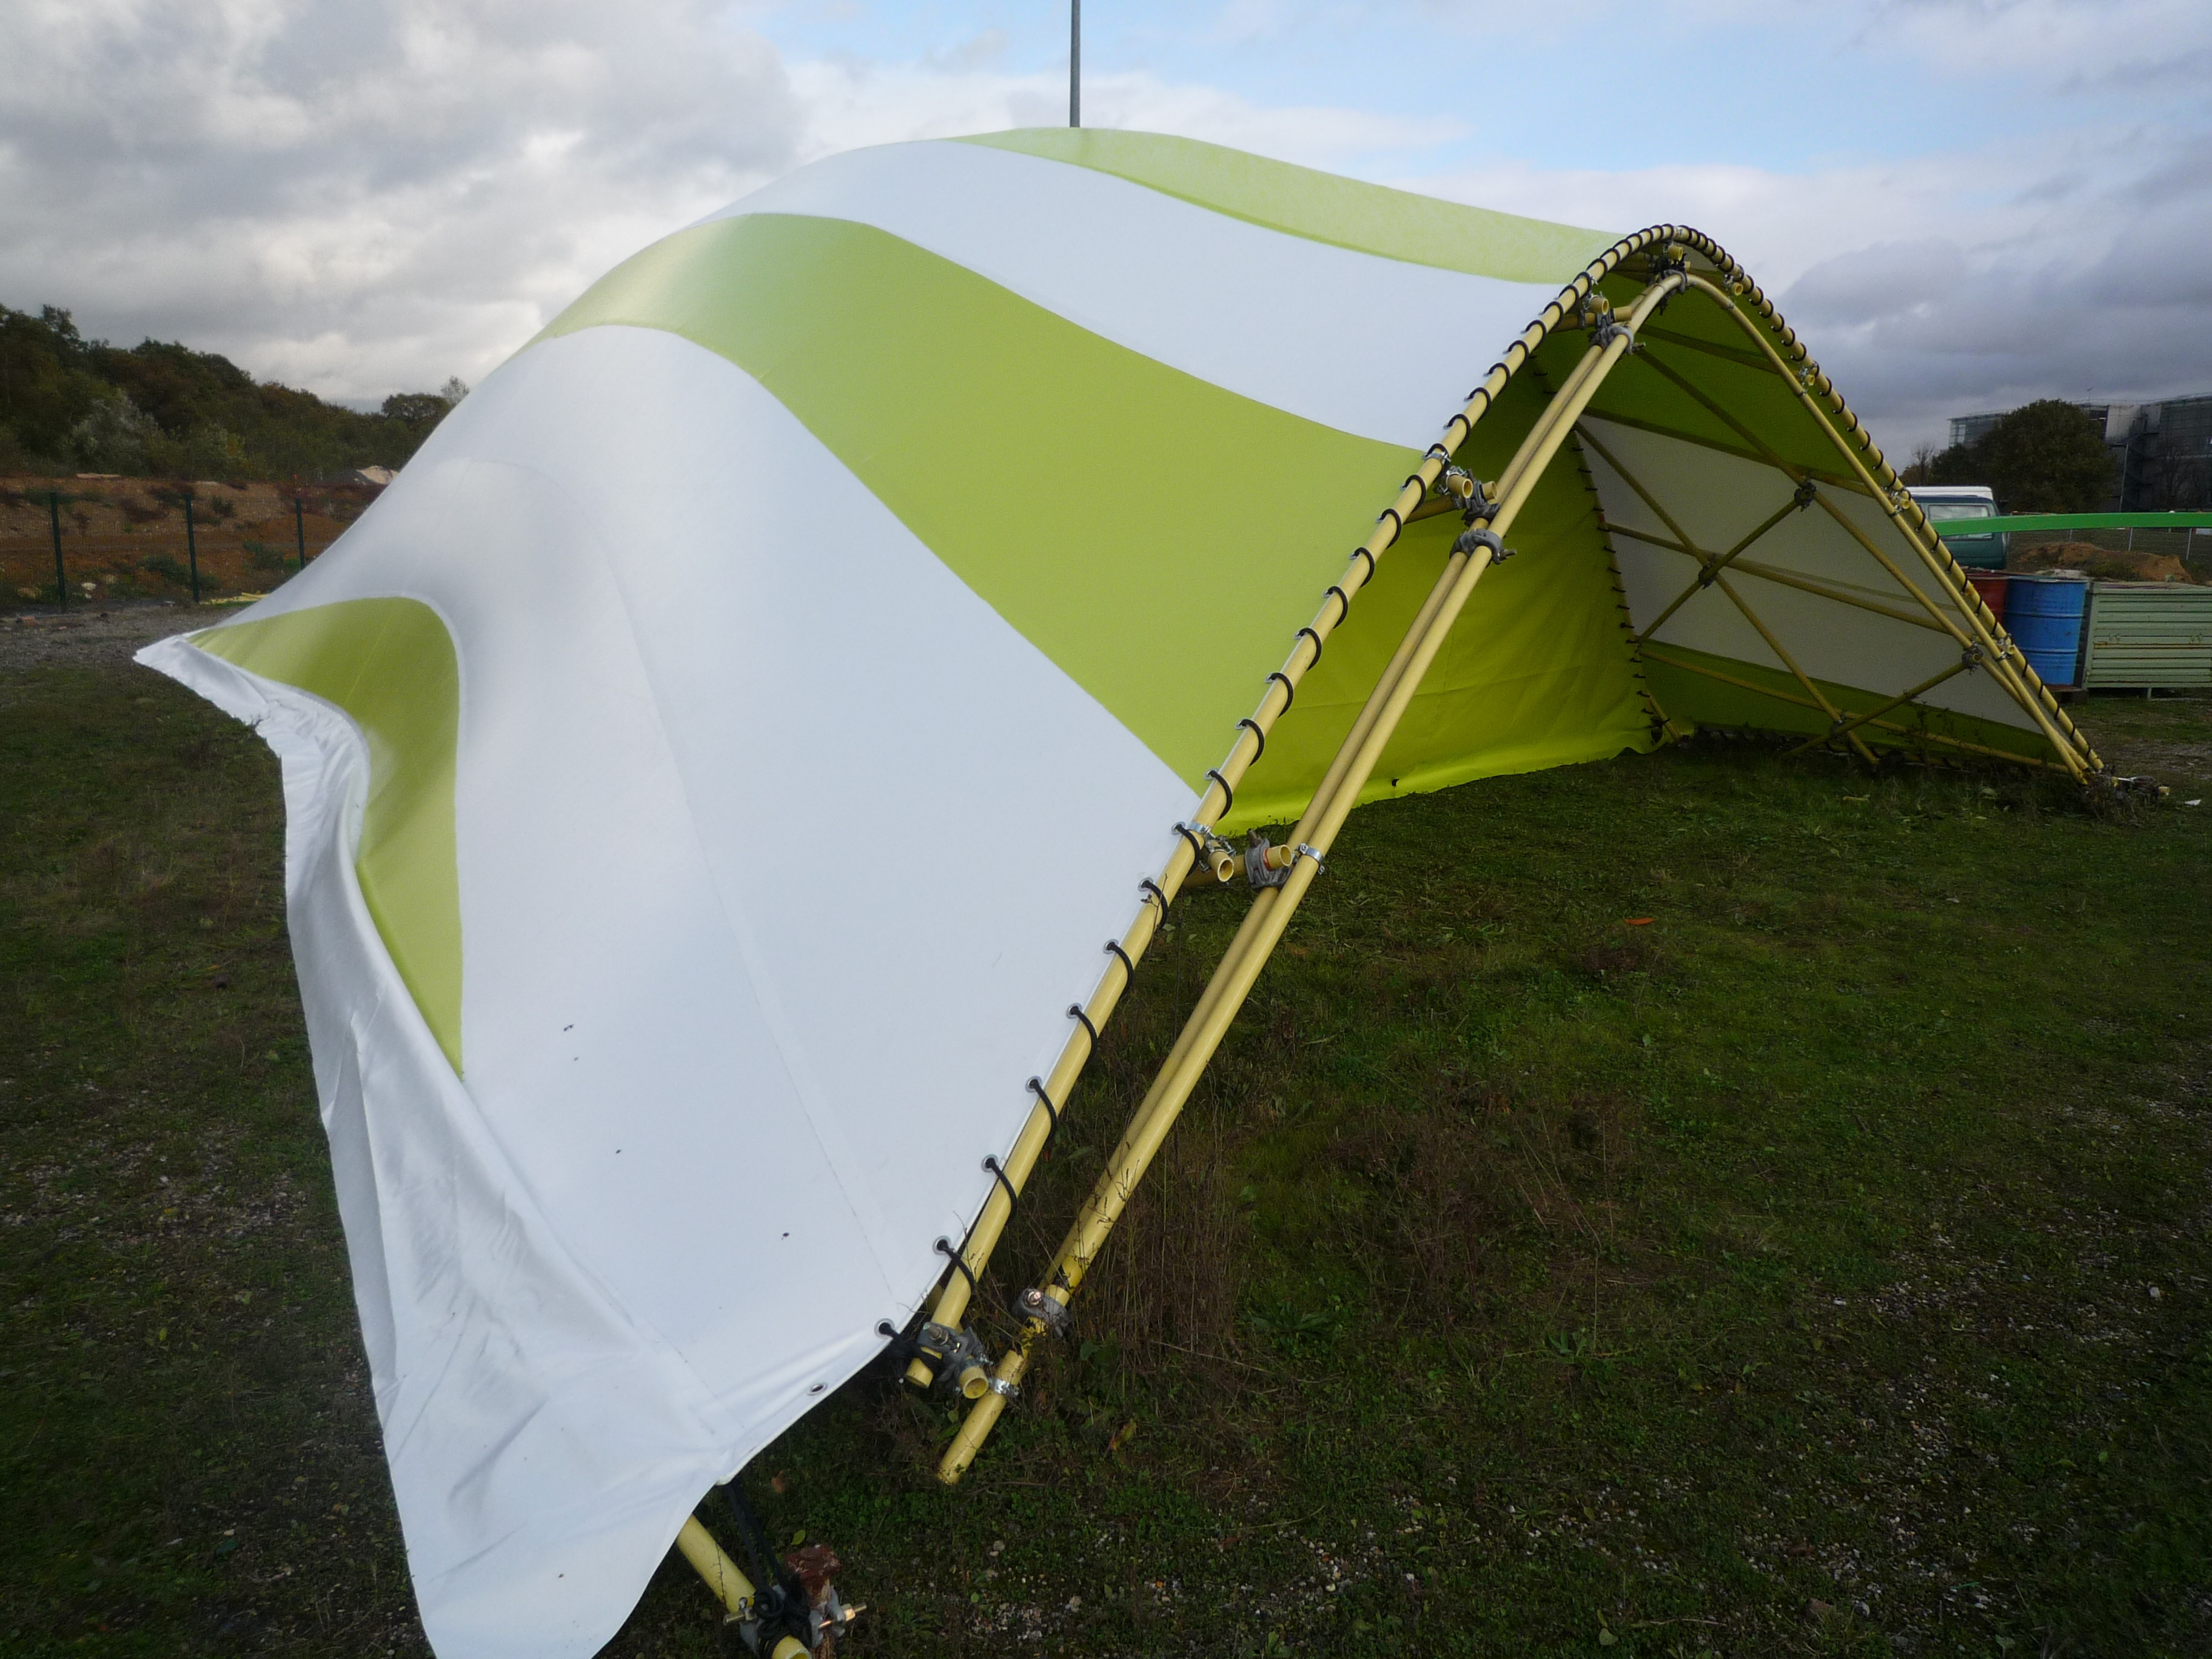
\includegraphics[width=0.48\textwidth]{proto_b.jpg}\label{fig:proto_b}}
		%
		\vspace{10pt}
		\caption{Prototypes and projects of GFRP elastic gridshells.}
		\label{fig:proto}    
\end{figure}
%
%\begin{figure}[p]
%	\begin{fullpage}
%		\captionsetup[subfloat]{captionskip=10pt}
%     		\centering
%     		%
%		\subfloat[][Mannheim (1975).]{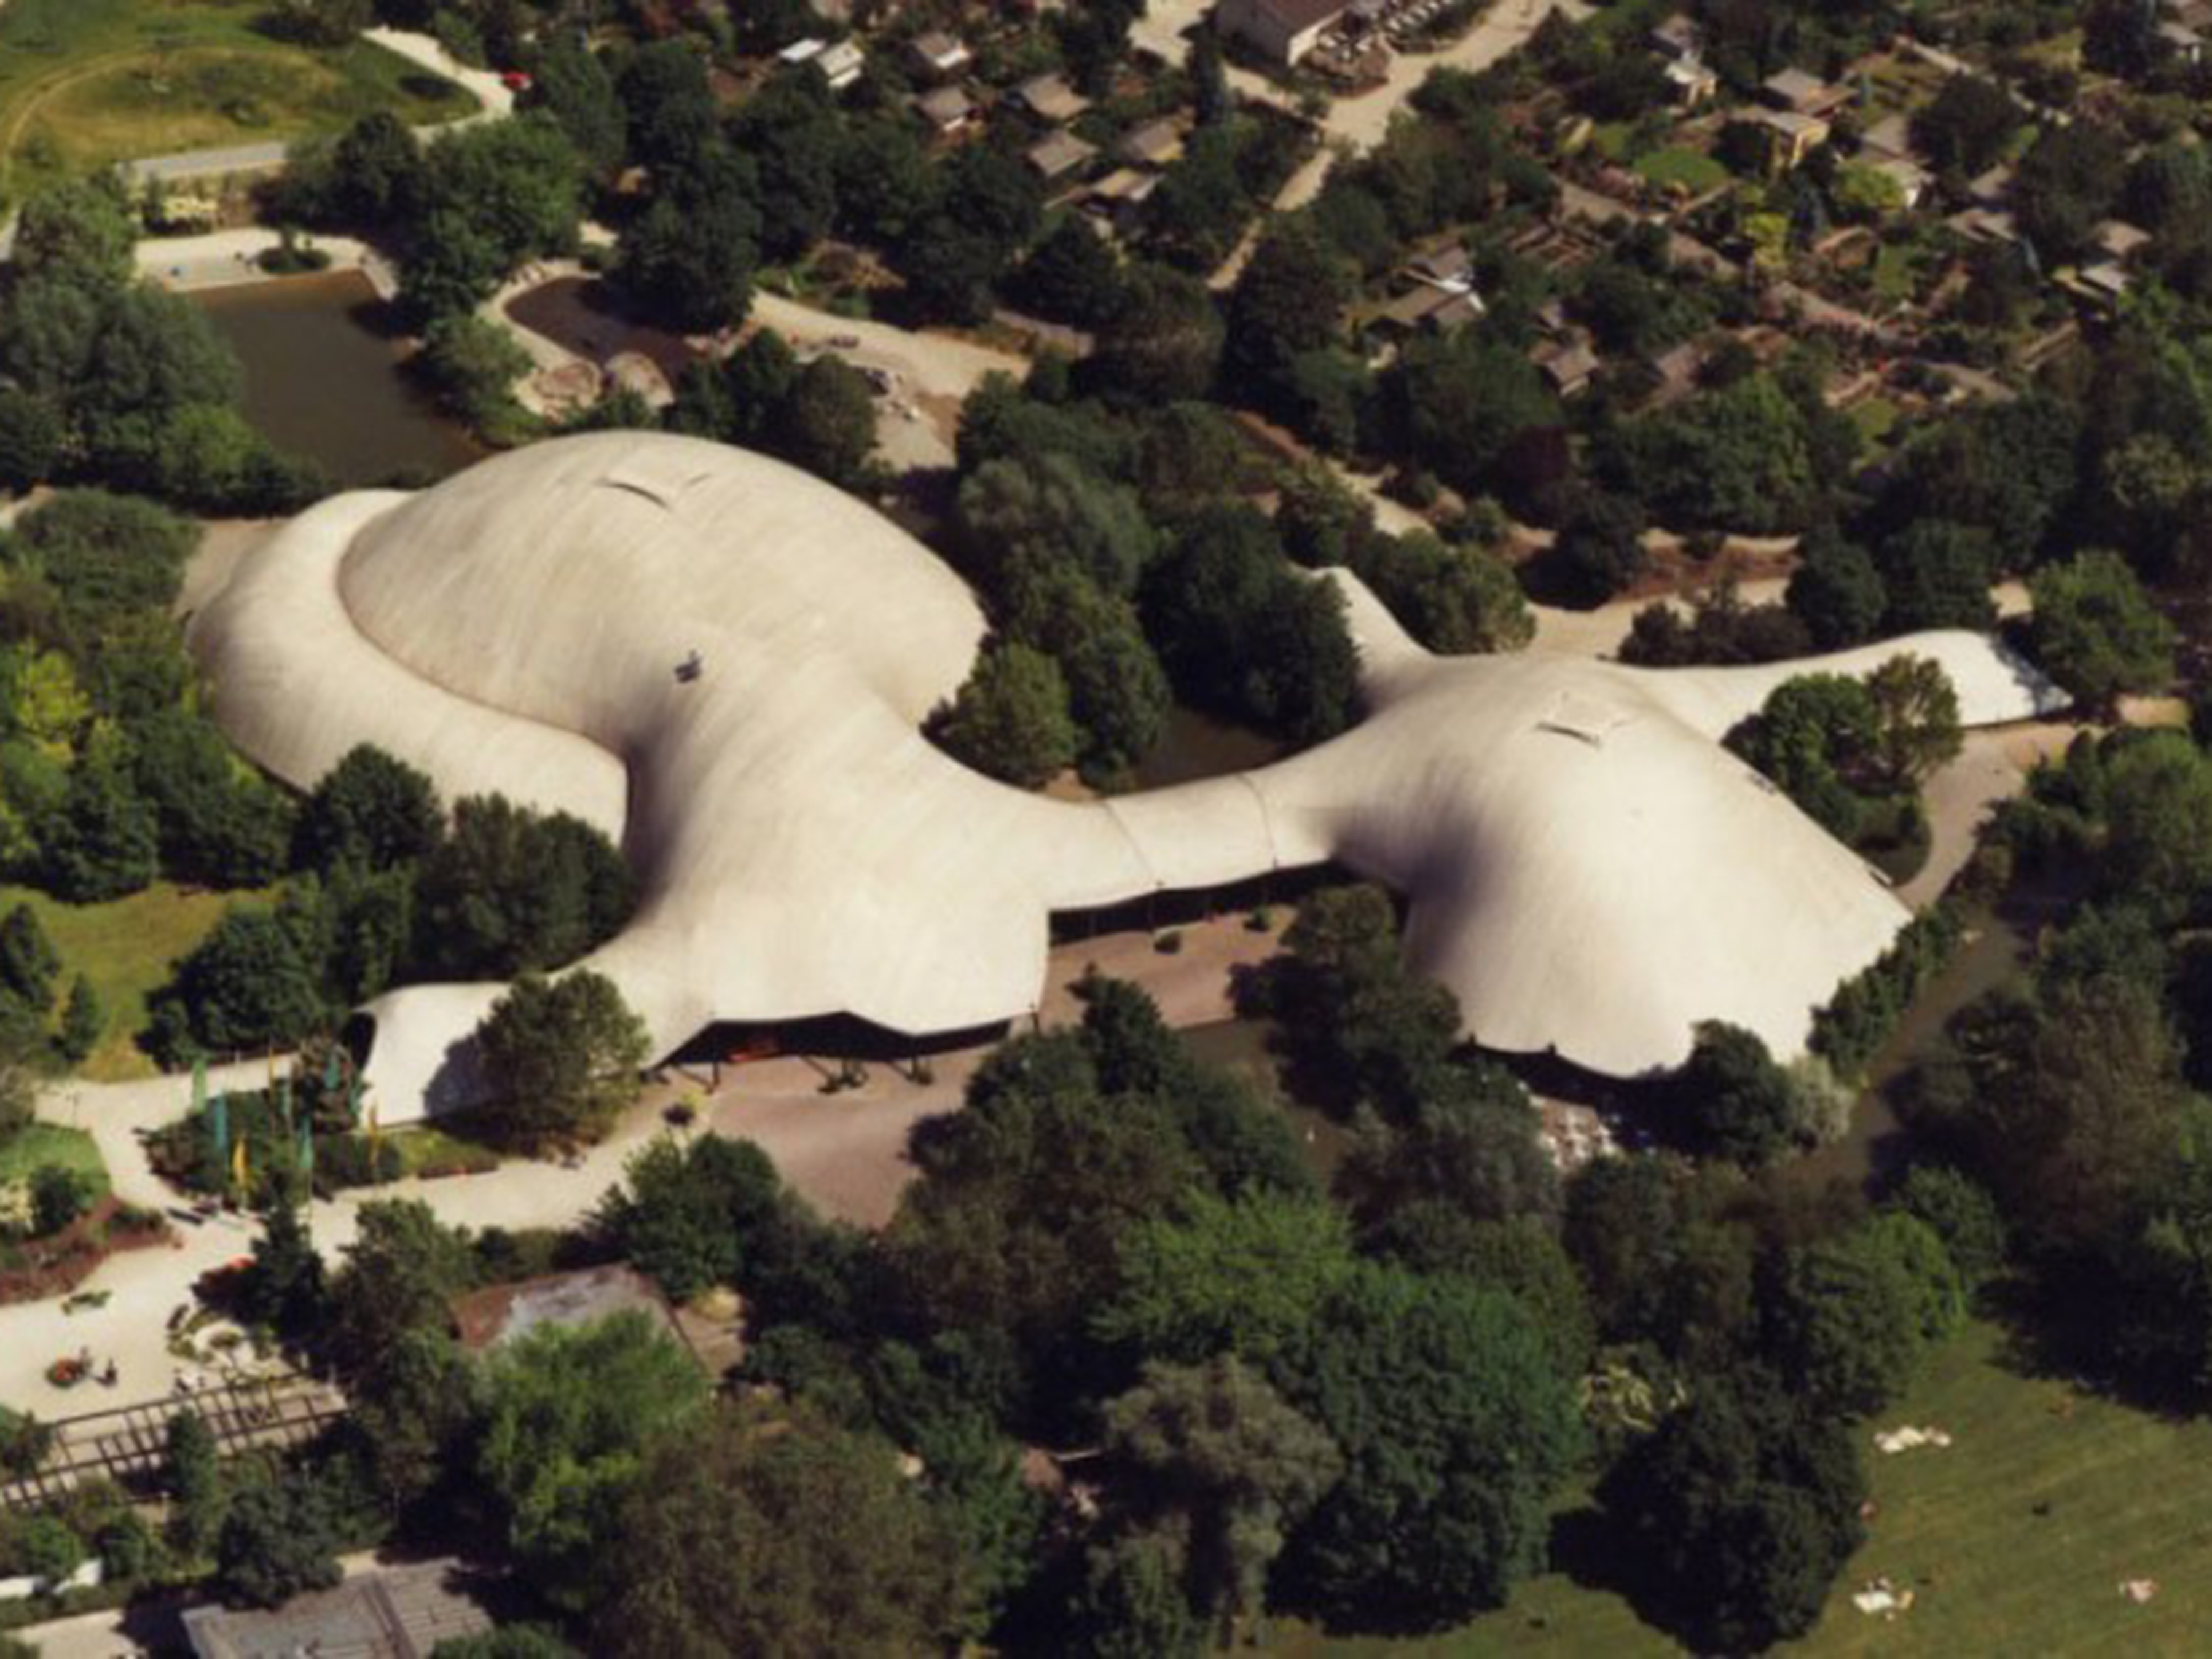
\includegraphics[width=0.48\textwidth]{mannheim_a.jpg}\label{fig:mannheim_a}}
%		\hspace*{\fill}
%		\subfloat[][Mannheim (1975).]{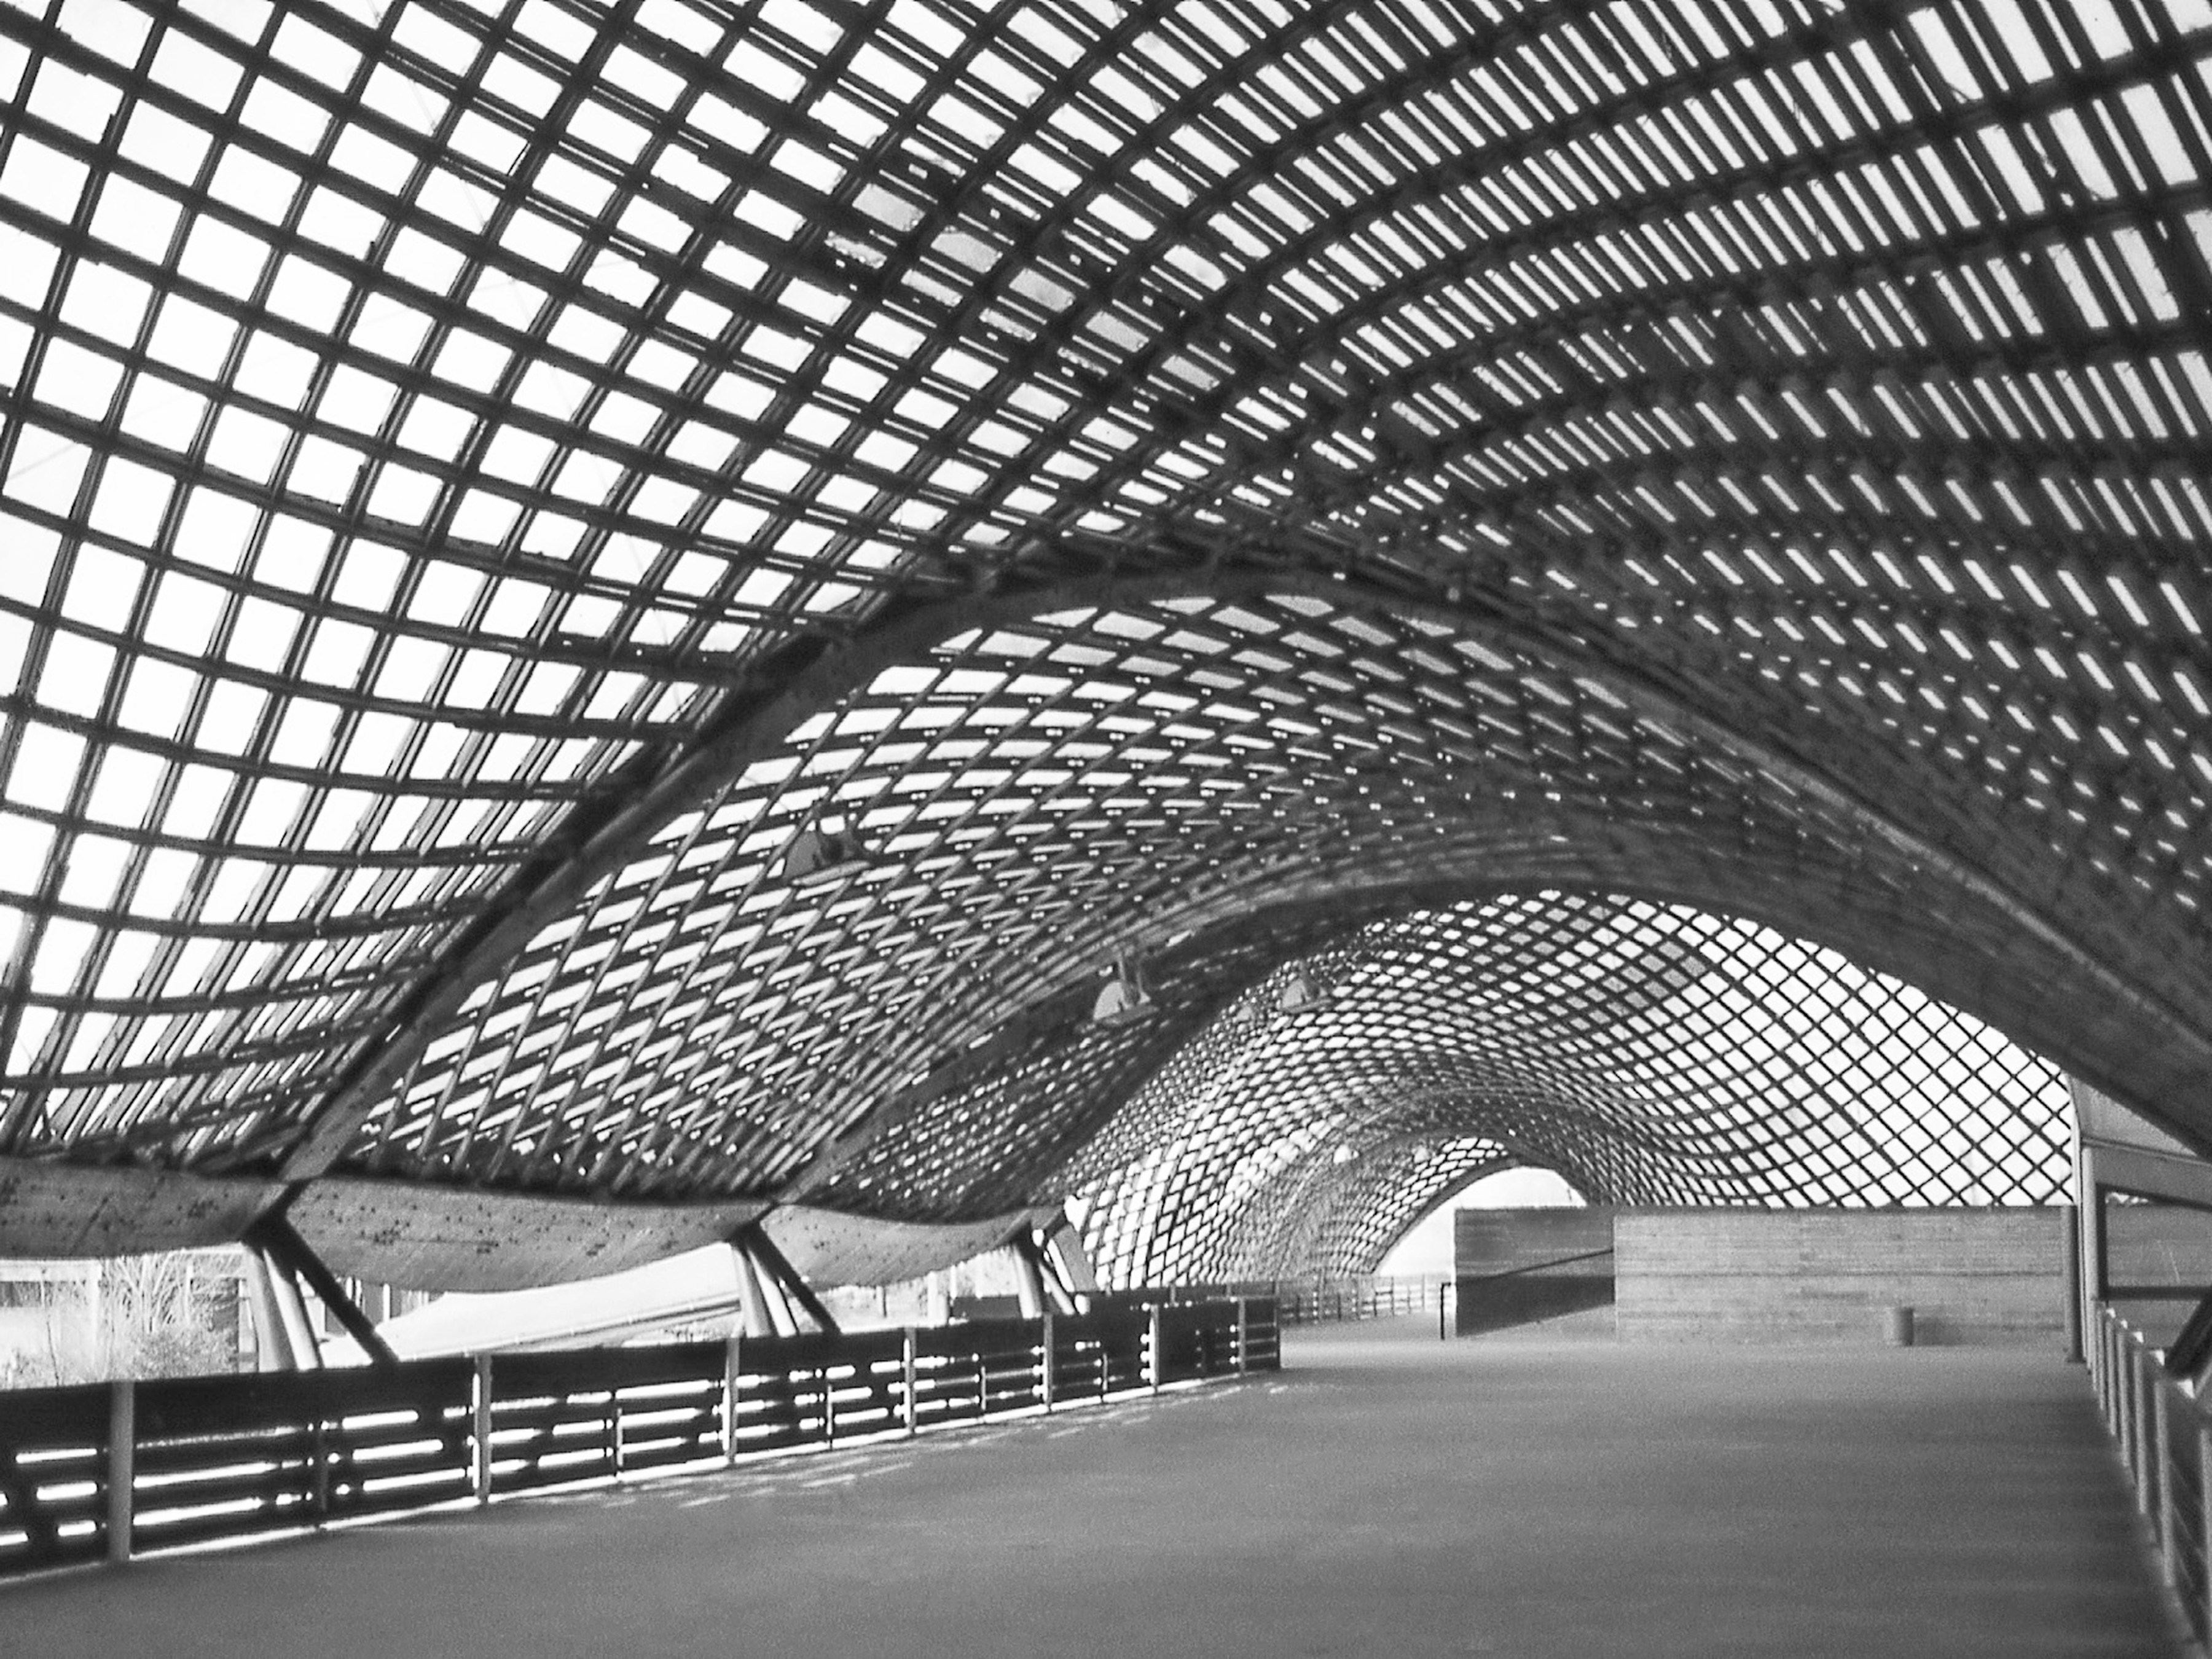
\includegraphics[width=0.48\textwidth]{mannheim_b.jpg}\label{fig:mannheim_b}} \\
%		%
%		\subfloat[][Downland (2002).]{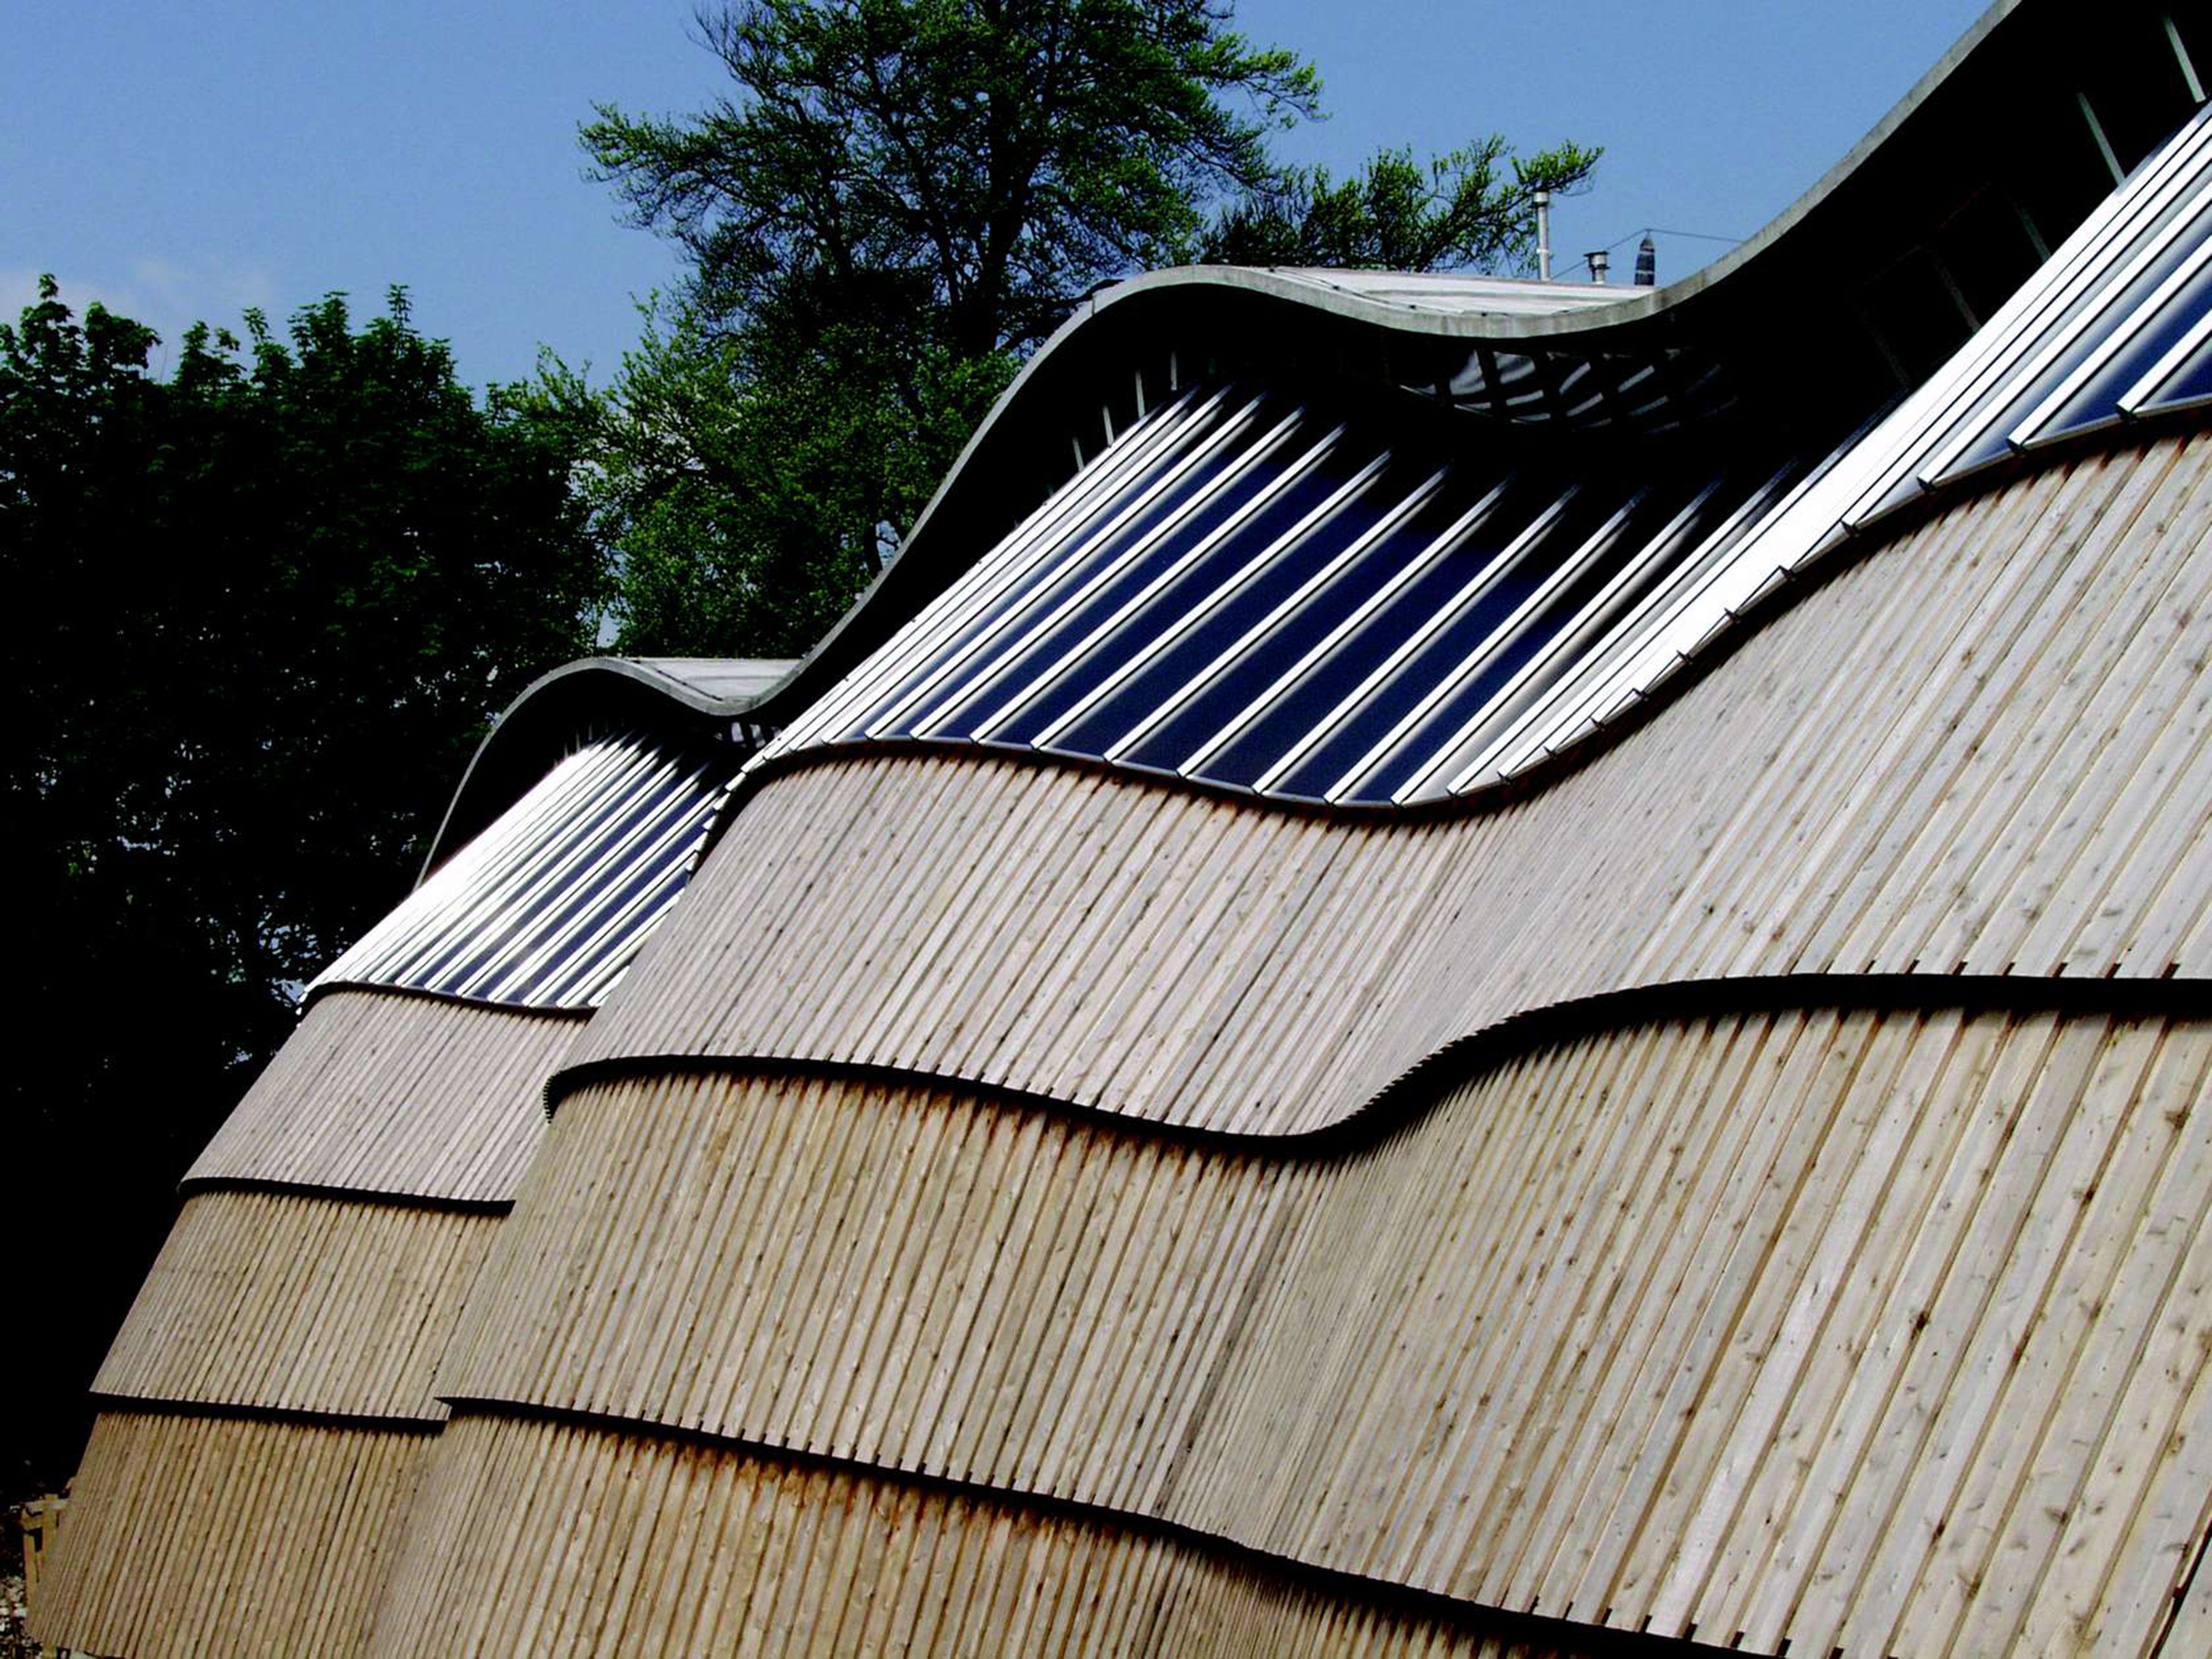
\includegraphics[width=0.48\textwidth]{downland_a.jpg}\label{fig:downland_a}}
%		\hspace*{\fill}
%		\subfloat[][Downland (2002).]{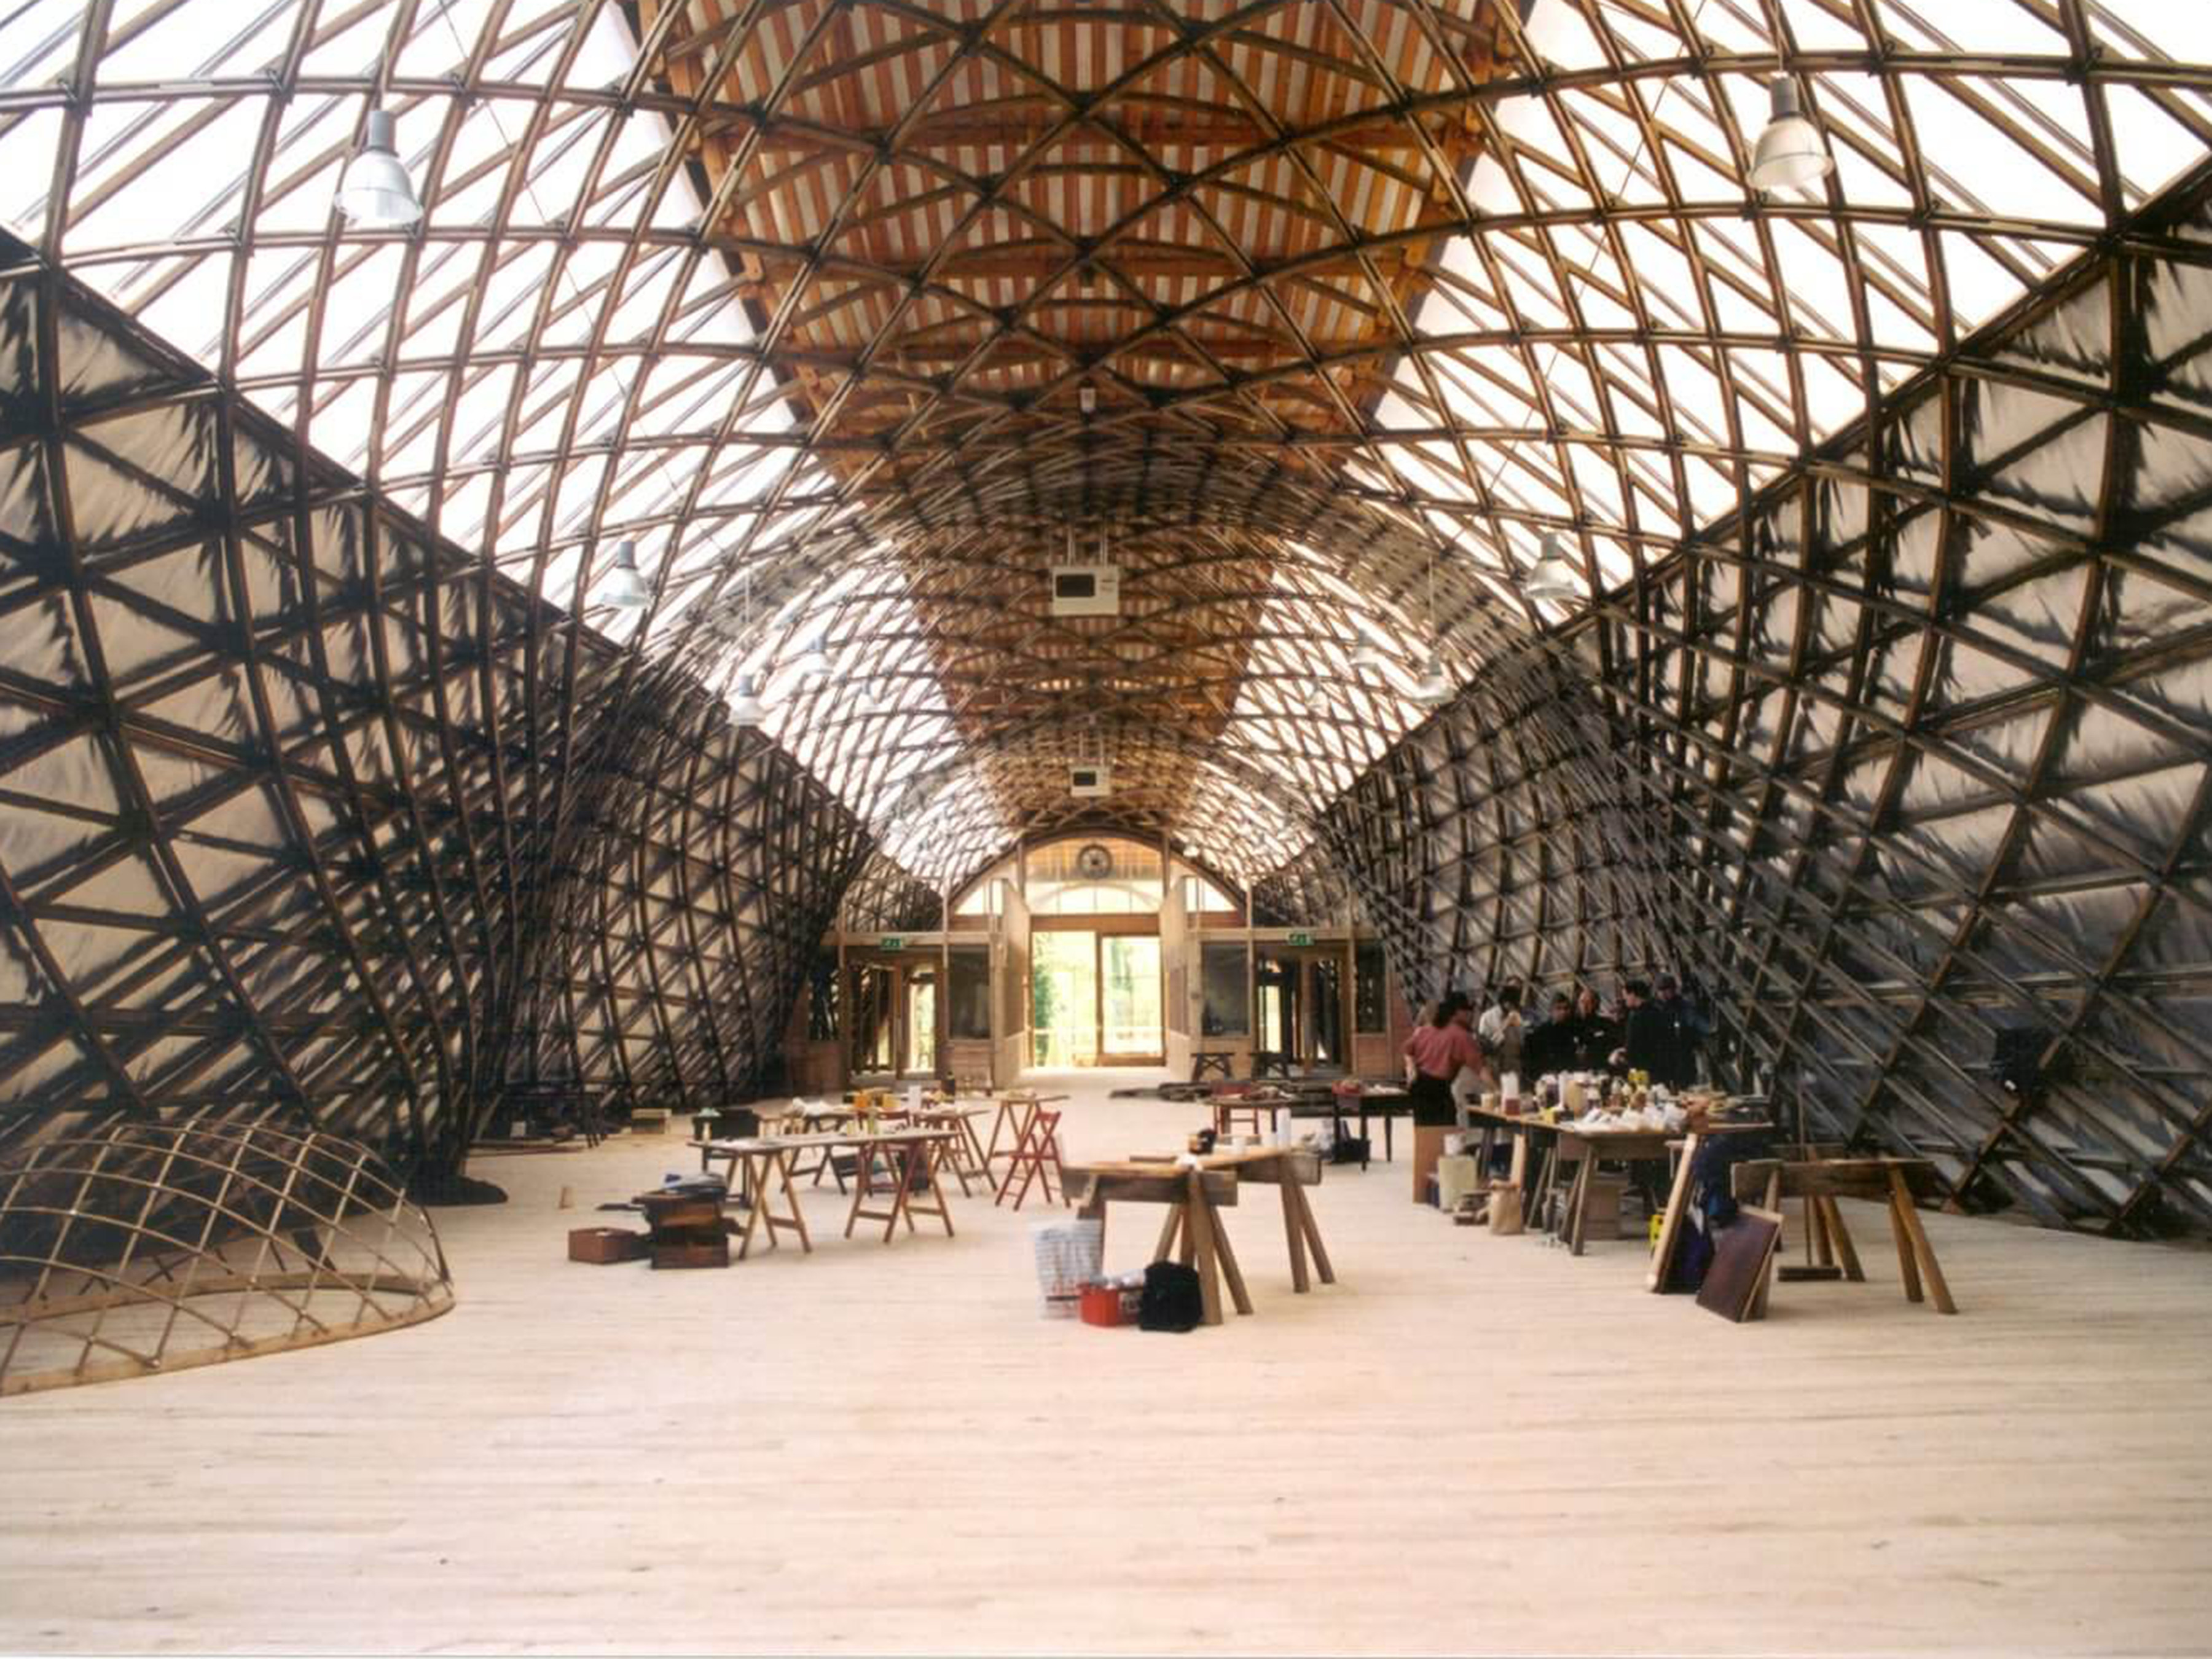
\includegraphics[width=0.48\textwidth]{downland_b.jpg}\label{fig:downland_b}} \\
%		%
%		\subfloat[][Savill (2006).]{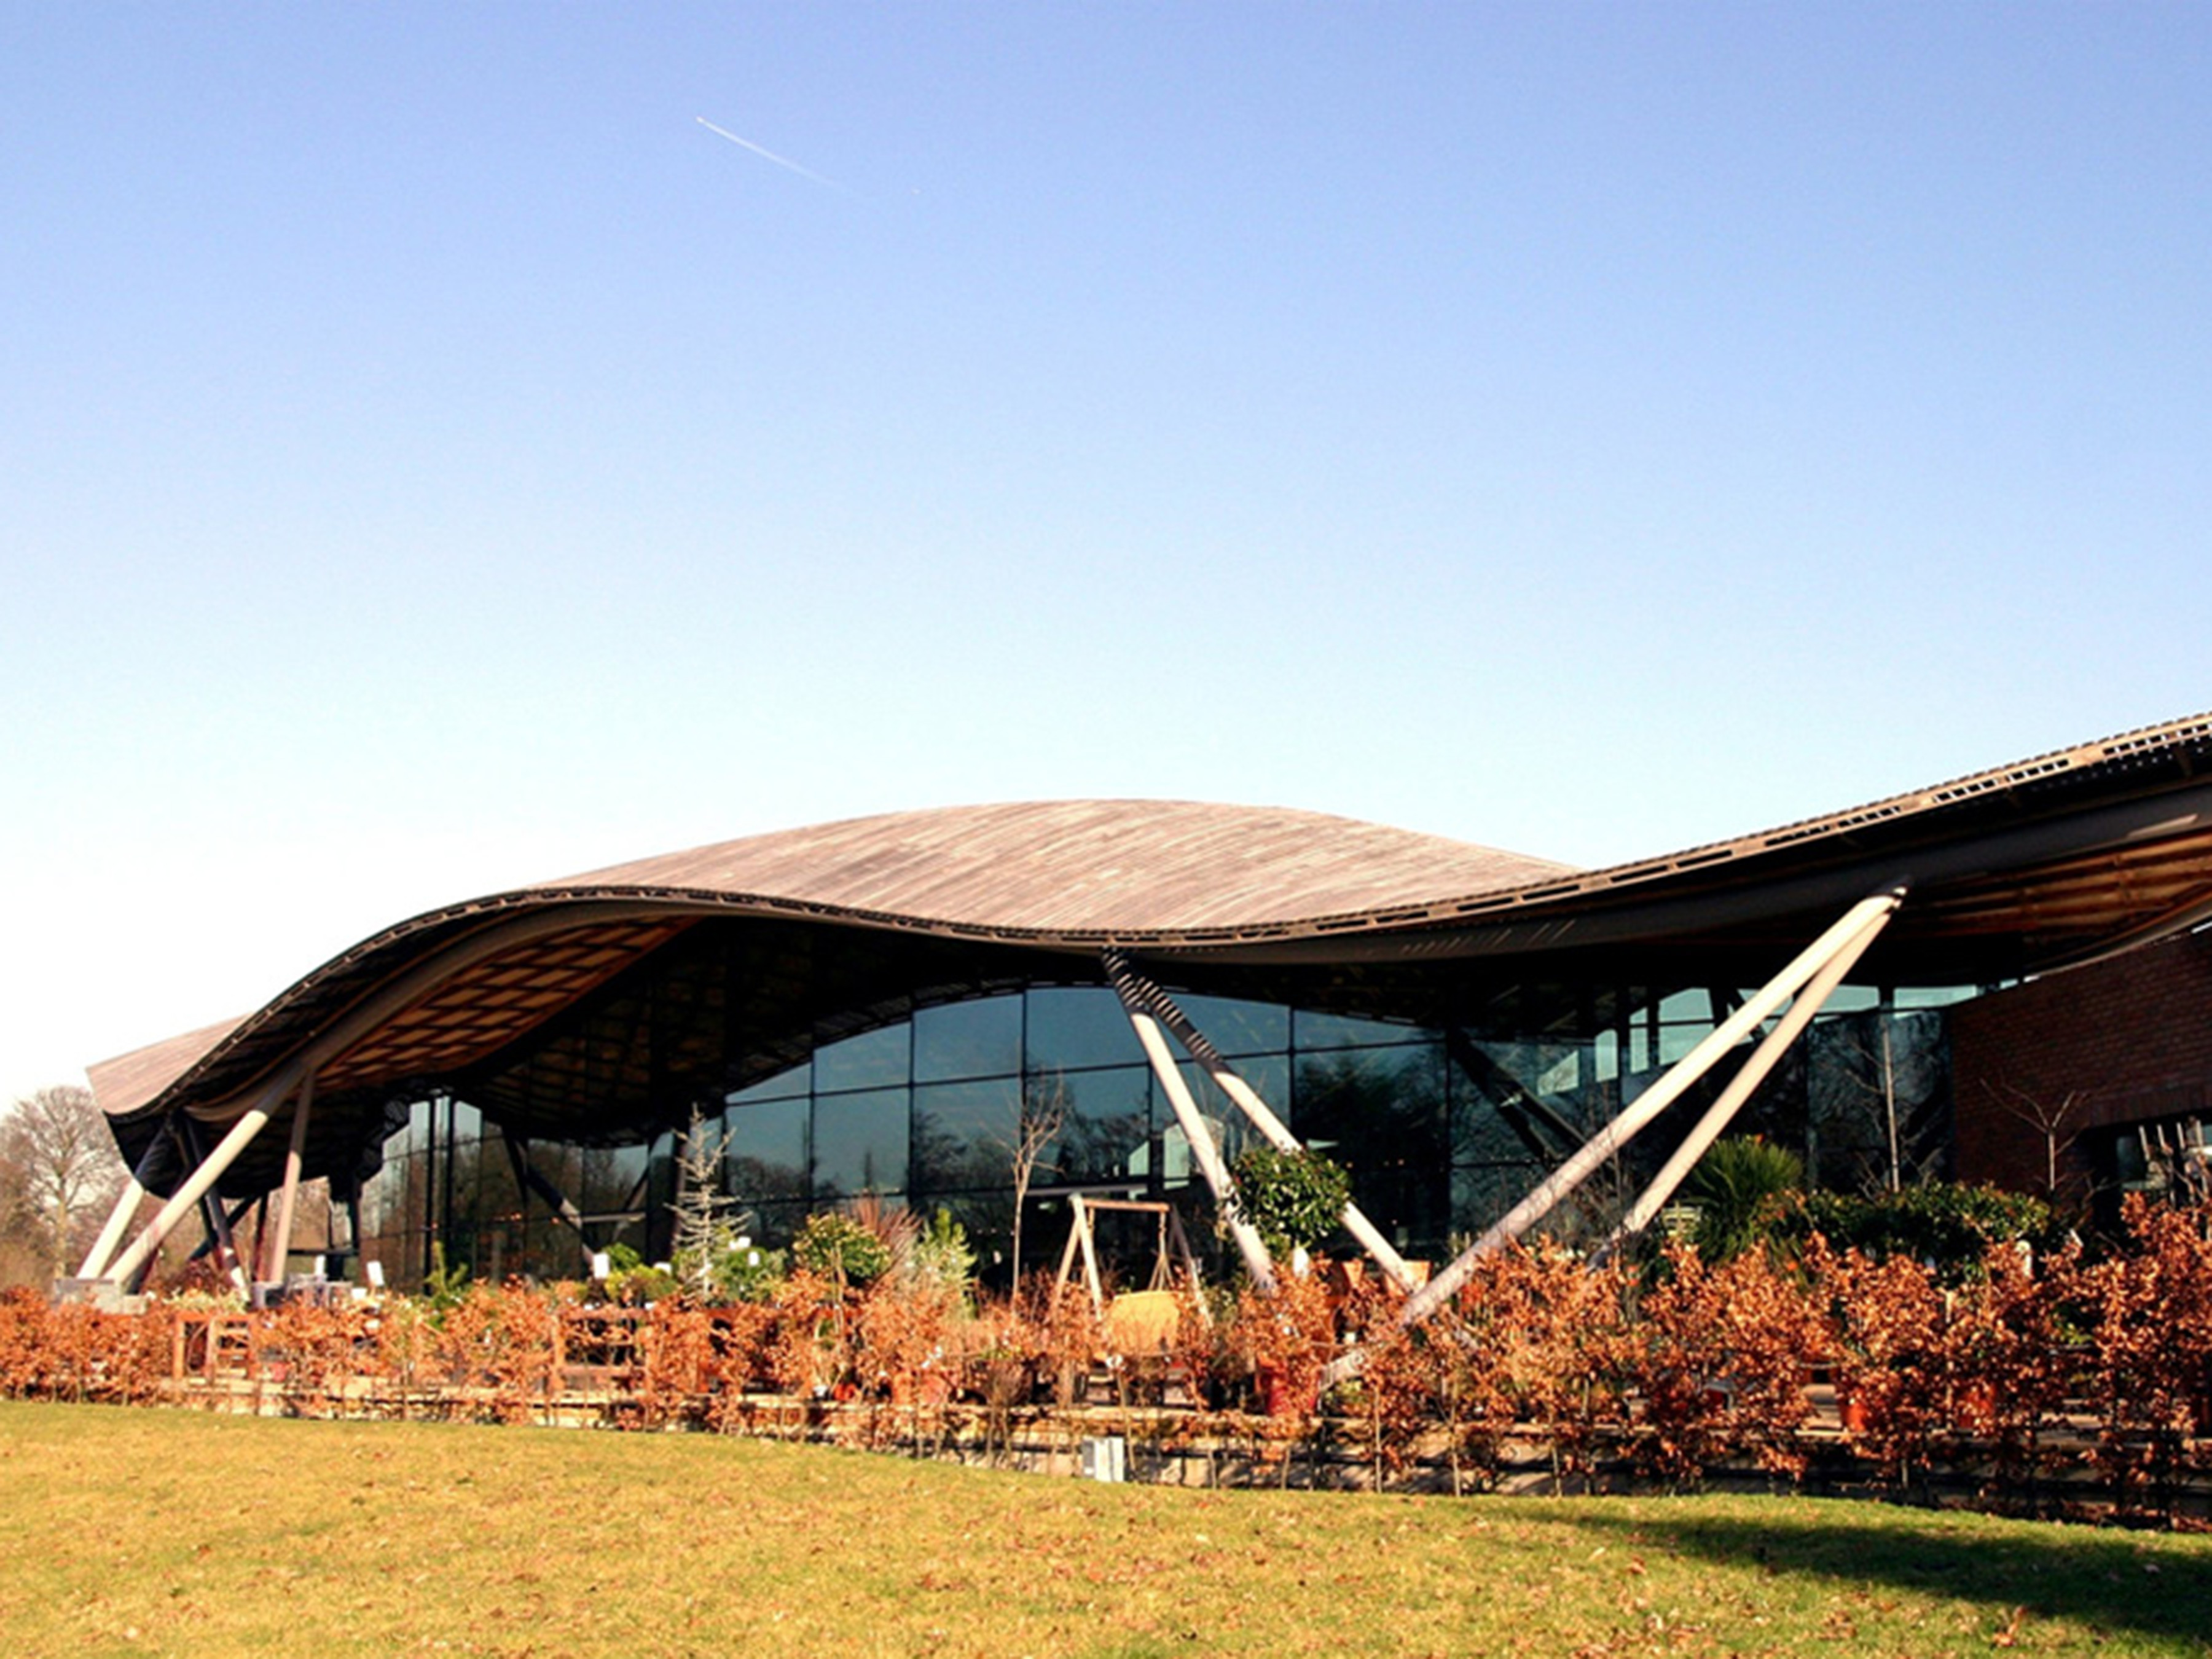
\includegraphics[width=0.48\textwidth]{savill_a.jpg}\label{fig:savill_a}}
%		\hspace*{\fill}
%		\subfloat[][Savill (2006).]{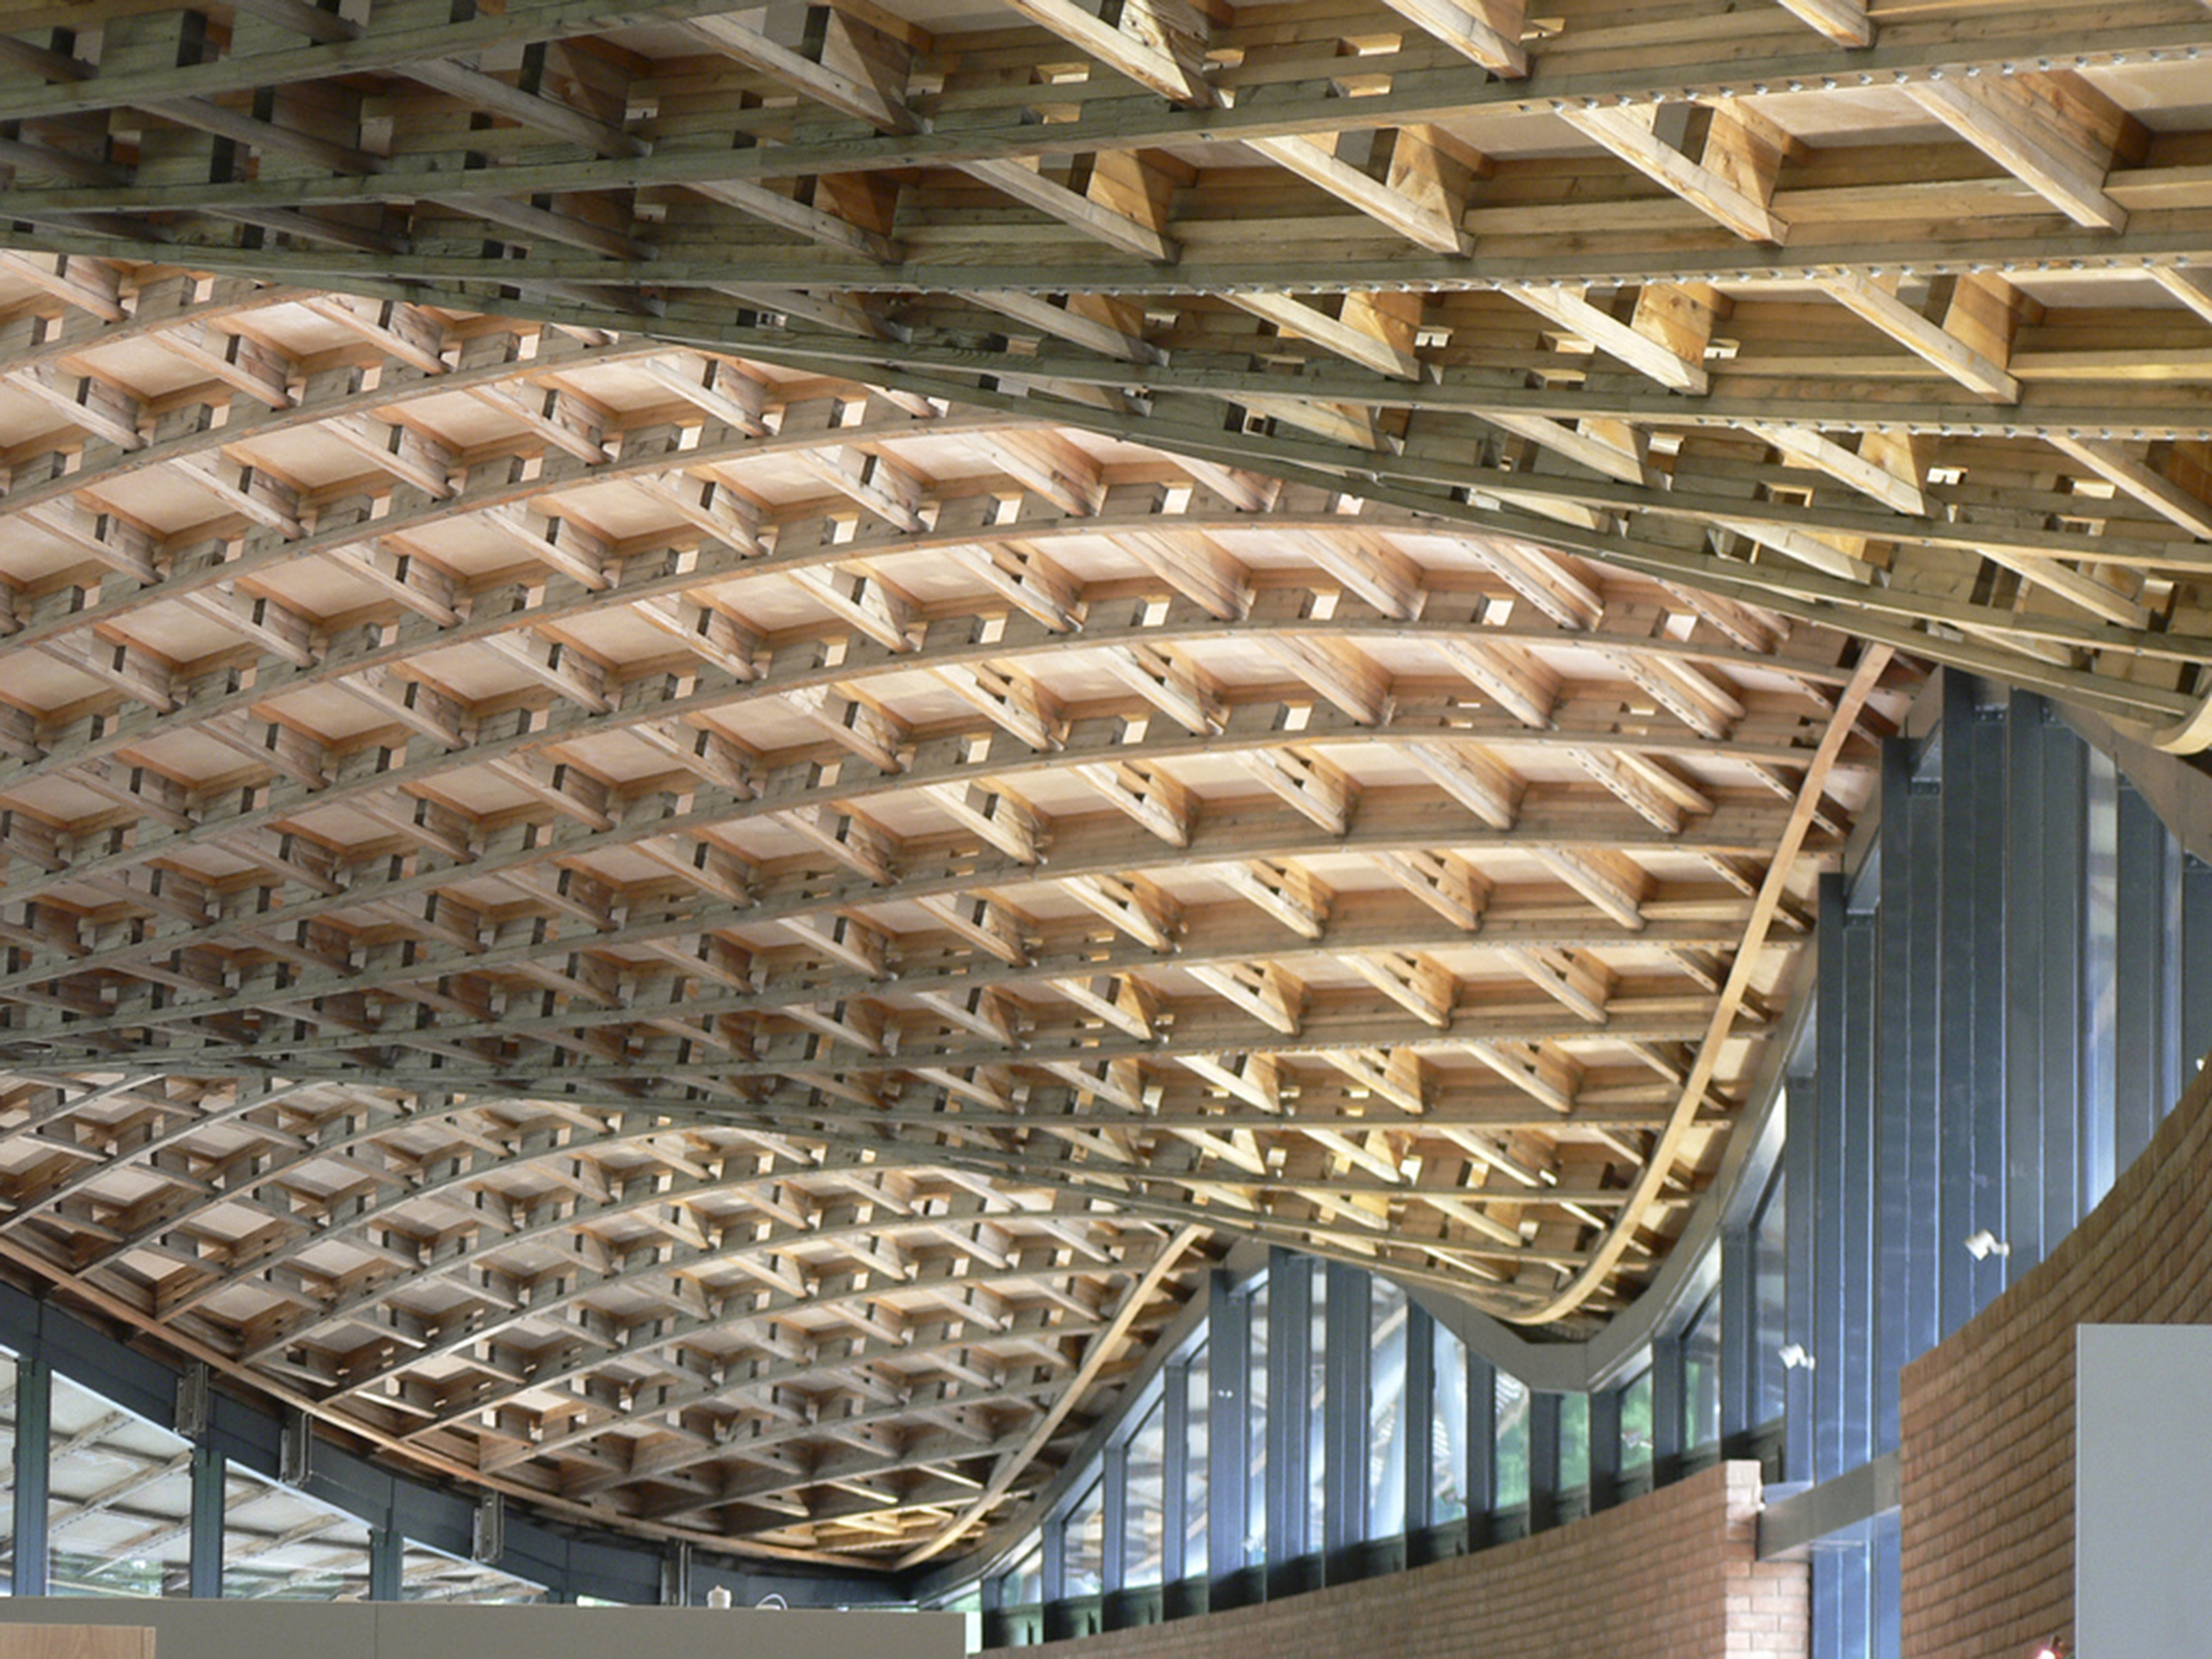
\includegraphics[width=0.48\textwidth]{savill_b.jpg}\label{fig:savill_b}}
%		%
%		\vspace{20pt}
%		\caption{Major permanent projects of elastic wooden gridshells built since 1975.}
%		\label{fig:projects}    
%	\end{fullpage}
%\end{figure}


\section{Elastic gridshells : revisiting Mannheim}


\section{Elastic gridshells : the benefits of composite materials}

Glass fiber reinforced polymer (GFRP) tubes are at the heart of the presented technology. They can favorably replace wood where both resistance and bending ability of the material is sought \cite{Douthe2010}. 

The tubes are made by pultrusion, \enquote{a continuous molding process whereby reinforcing fibers are saturated with a liquid polymer resin and then carefully formed and pulled through a heated die to form a part. Pultrusion results in straight constant cross section parts of virtually any shippable length}.\footnote{Video explaining the pultrusion process~: \url{https://www.youtube.com/watch?v=4MoHNZB5b_Y}} This process is very economic and its standardization guarantees very stable material and mechanical properties. It frees designers from the problem of joining wood pieces with finger joints to obtain long and continuous members and of wood durability.

\begin{figure}[h]
	\centering
		\captionsetup[subfloat]{captionskip=10pt}
		\subfloat[][Forum Café, Solidays (2011).]{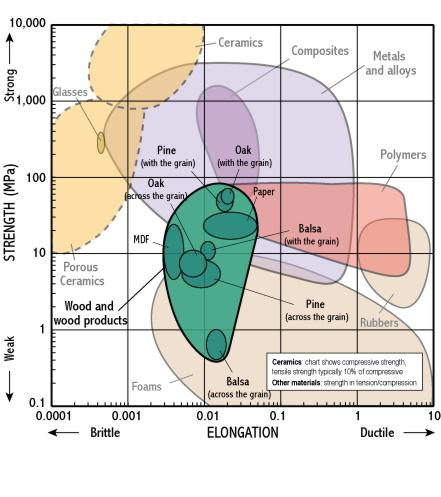
\includegraphics[width=0.6\textwidth]{ashby_woods.jpg}\label{fig:asby_co}}
		\\ \vspace{1cm}
		\subfloat[][Prototype (2007).]{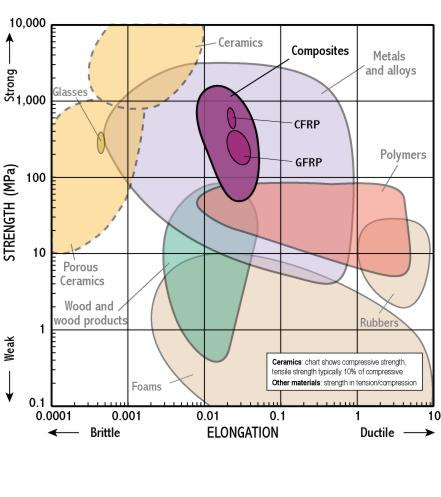
\includegraphics[width=0.6\textwidth]{ashby_composites.jpg}\label{fig:proto_a}}
		%
		\vspace{10pt}
		\caption{Prototypes and projects of GFRP elastic gridshells.}
		\label{fig:proto}    
\end{figure}




\subsection{Recent developments}
% ------------------------------------------
The Faraday Pavilion : \cite{Nicholas2013}
The Pishwanton / lothian : \cite{Pishwanton2003}
The laboratory Navier tested various numerical methods to generate such grids \cite{Bouhaya2009}
Masson :  \cite{Masson2017}.
\begin{figure}[t]
	\centering
		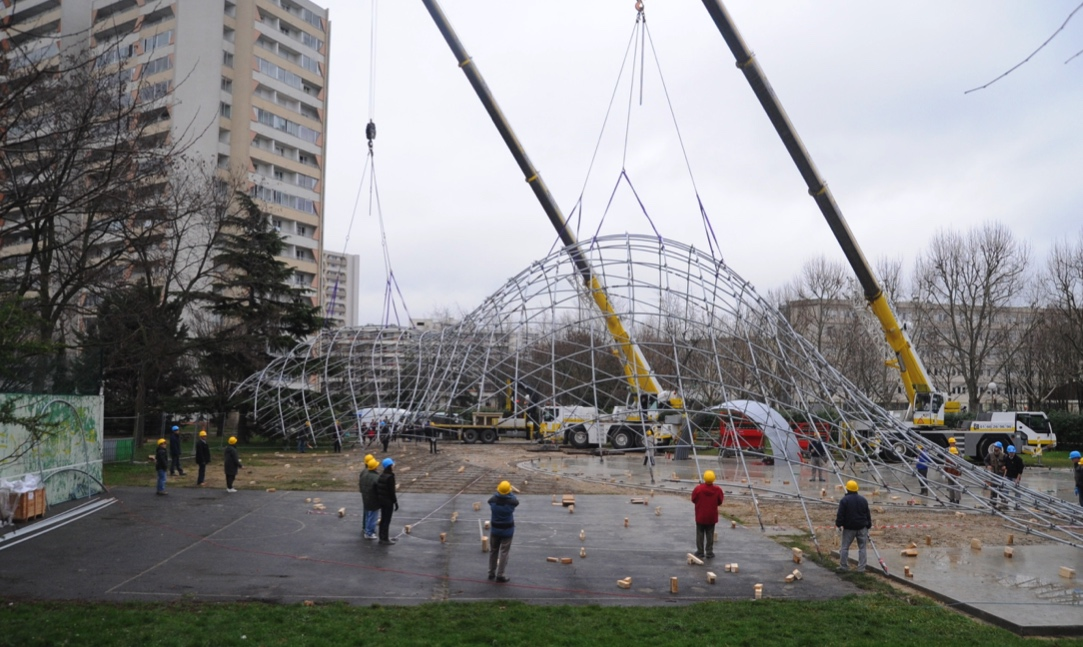
\includegraphics[width=\textwidth]{image6}
	\caption{Erection of the primary grid by two cranes}
	\label{fig:5}
\end{figure}



\subsection{Gridshell in composite material}
% ------------------------------------------

The benefits of GFRP gridshells have been covered previously. We just recall the main aspects.

The gridshells built in composite material, being at the heart of this paper, are consistent with the framework defined previously, that is to say :


Glass fiber reinforced polymer (GFRP) tubes are at the heart of the presented technology. They can favorably replace wood where both resistance and bending ability of the material is sought \cite{Douthe2010}. 

The tubes are made by pultrusion, \enquote{a continuous molding process whereby reinforcing fibers are saturated with a liquid polymer resin and then carefully formed and pulled through a heated die to form a part. Pultrusion results in straight constant cross section parts of virtually any shippable length}.\footnote{Video explaining the pultrusion process~: \url{https://www.youtube.com/watch?v=4MoHNZB5b_Y}} This process is very economic and its standardization guarantees very stable material and mechanical properties. It frees designers from the problem of joining wood pieces with finger joints to obtain long and continuous members and of wood durability. 


\subsubsection{Structural Typology}
% ------------------------------------------
Their mechanical behaviour is very similar to the one of real shells even if the material is discrete and located in a grid more or less open. In spite of that, gridshells benefit from the same advantages as the ones showed by an eggshell : they can cross large span using a low amount of material. Their stiffness is mainly linked to their double-curved shape.


\subsubsection{Material Flexibility for Structural Rigidity}
% ------------------------------------------
In this field of application, composite materials like glass fibre reinforced polymer (GFRP) could favourably replace wood, where both resistance and bending ability of the material is sought \cite{Douthe2010}. The stiffness of the structure does not derive from the intrinsic material rigidity but principally from its geometric curvature. Ideally, the composite profiles are produced by pultrusion, an economic continuous moulded process. The standardization of the process guaranties very stable material and mechanical properties. It frees designers from the painful problematic of wood joining and wood durability. The characterization of this material is presented further in the paper.


\subsubsection{Erection Process}
% ------------------------------------------
Usually, the grid morphology is not trivial and leads to design numerous costly and complex joints. To overcome this issue, an original and innovative erection process was developed that takes advantage of the flexibility inherent to slender elements. A regular planar grid made of long continuous linear members is built on the ground (\autoref{fig:6}a). The elements are pinned together so the grid has no in-plane shear stiffness and can accommodate large-scale deformations during erection. Then, the grid is bent elastically to its final shape (\autoref{fig:5}). Finally, the grid is frozen in the desired shape with a third layer of bracing members (\autoref{fig:6}b) and the structure becomes a shell.
\begin{figure}[t]
	\begin{minipage}[b]{.70\linewidth}
		\centering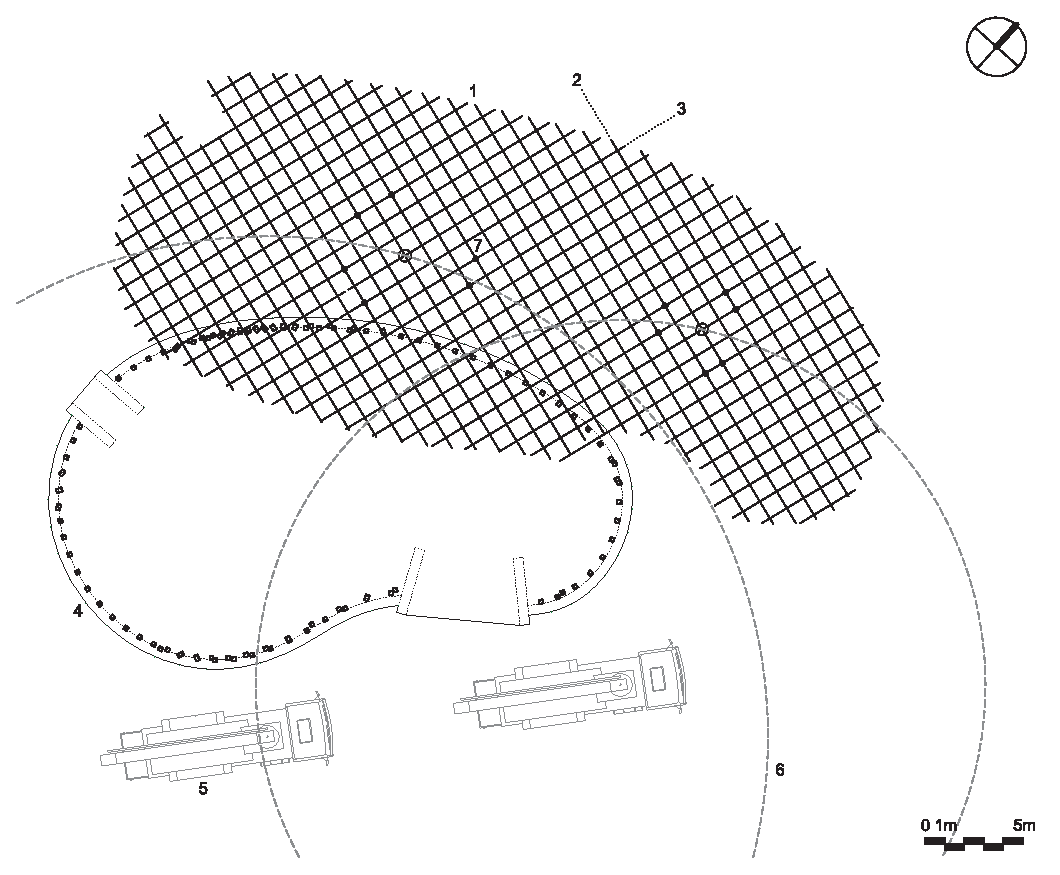
\includegraphics[width=0.95\textwidth]{image5}
	\end{minipage} \hfill
	\begin{minipage}[b]{.25\linewidth}
		\centering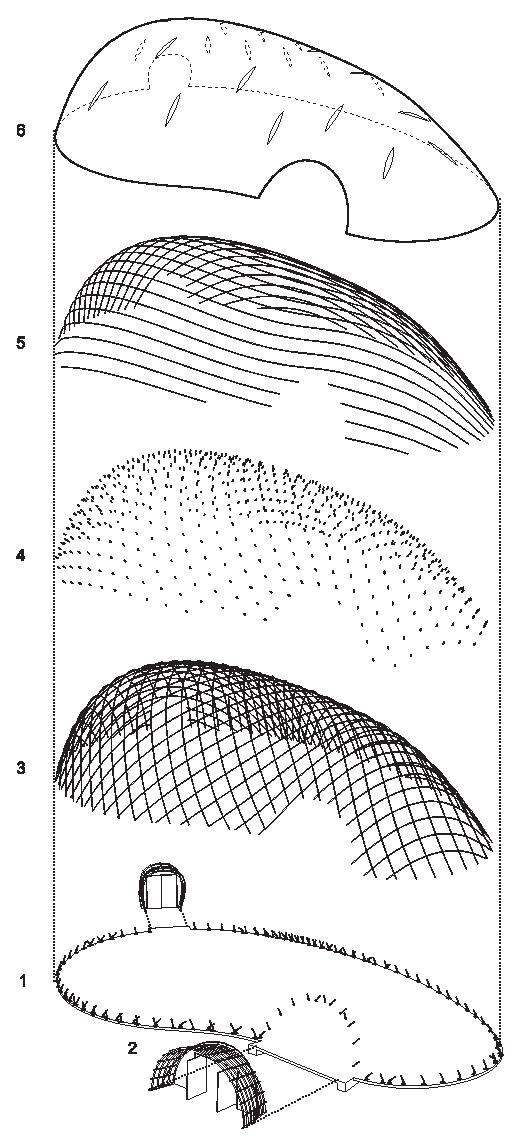
\includegraphics[width=0.93\textwidth]{image9}	
	\end{minipage}
	\vspace{0.5cm}
	\caption{Erection plan and construction stages}\label{fig:6}
\end{figure}

%\bibliographystyle{alpha}
%\bibliography{../library}

